% LaTeX-Vorlage zur Erstellung einer Abschlussarbeit in der Fakultät Elektrotechnik, Medien und Informatik an der OTH Amberg-Weiden
% Diese Vorlage entstand im Rahmen des Kurses "LaTeX fürs Studium"
% Aktuelle Version: v0.02
% Stand: 06.08.2015
%
% Changelog:
%
% v0.02: 06.08.2015, Anpassung der Vorlage:
% + Persönliche Informationen (Vorname, Name, Titel usw.) werden direkt in die PDF-Dokumenteinstellungen übernommen
% + Korrektur der Verlinkung von Abbildungs- und Tabellenverzeichnis aus dem Inhaltsverzeichnis (phantomsection) bzw. deren Seitenzahl
%   Besten Dank für diesen Hinweis an Jan-Olaf Becker
% + Anpassung des Namens der Fakultät nach deren Umbenennung
%
% v0.01: 14.03.2012, Erstellung der Vorlage

\documentclass[12pt,oneside]{report}
\usepackage[T1]{fontenc}		% Einstellungen fuer Umlaute usw.
\usepackage[utf8x]{inputenc}
\usepackage[ngerman]{babel}

\usepackage{parskip}			% Einstellungen fuer Absaetze: Abstand statt Einrueckung

\usepackage[a4paper,			% Papierformat A4
	    left=2.5cm,				% linker Rand
	    right=2.5cm,			% rechter Rand
	    top=1.5cm,				% oberer Rand
	    bottom=1.5cm,			% unter Rand
	    marginparsep=5mm,		% Abstand der Randnotizen
	    marginparwidth=10mm, 	% Breite der Randnotizen
	    headheight=7mm,			% Hoehe der Kopfzeile
	    headsep=1.2cm,			% Abstand der Kopfzeile
	    footskip=1.5cm,			% Abstand der Fusszeile
	    includeheadfoot]{geometry}

\usepackage{fancyhdr}						% Konfiguration von Kopf- und Fusszeilen
\pagestyle{fancy}							% Seitenstil 'fancy'
\fancyhf{}									% vorhandene Einstellungen loeschen
\setlength{\headwidth}{\textwidth}			% Kopf- und Fusszeile so breit wie der Haupttext
\fancyfoot[R]{\thepage} 					% Festlegung des Seitenstils: Seitenzahlen in der Fusszeile rechts
\fancyfoot[L]{\leftmark}					% Kapitelnr. und -Bezeichnung in der Fusszeile links
\fancyhead[R]{\IhreArbeit}					% "Bachelorarbeit" in der Kopfzeile rechts
\fancyhead[L]{\IhrVorname\ \IhrNachname}	% Vorname und Name in der Kopfzeile links
\renewcommand{\chaptermark}[1]{			% Definition der Ausgabe des Kapitels
  \markboth{Kapitel \thechapter. #1}{}}
\renewcommand{\headrulewidth}{0.5pt}		% Trennlinie zwischen Kopfzeile und Haupttext
\renewcommand{\footrulewidth}{0.5pt}		% Trennlinie zwischen Haupttext und Fusszeile
\fancypagestyle{plain}{					% Anpassung des Seitenstils 'plain' bei Beginn neuer Kapitel
  \fancyhf{}								% Vorbelegung loeschen
  \fancyfoot[C]{\thepage}					% Seitenzeilen in der Fusszeile mittig
  \fancyhead[R]{\IhreArbeit}				% "Bachelorarbeit" in der Kopfzeile rechts
  \fancyhead[L]{\IhrVorname\ \IhrNachname}	% Vorname und Name in der Kopfzeile links
}

\usepackage{amsmath}			% Pakete fuer den Mathematikmodus
\usepackage{amssymb}
\usepackage[intlimits]{empheq}

\usepackage[sc]{mathpazo}		% Schriftart Palatino fuer Haupttext und Mathematikmodus
\usepackage{pifont}				% zusaetzliche Symbole

\usepackage[format=hang,		% Einstellung fuer Bildunterschriften
            font={footnotesize},
            labelfont={bf},
            margin=1cm,
            aboveskip=5pt,
            position=bottom]{caption}

\usepackage{graphicx}							% Einbinden von Graphiken
\usepackage[svgnames,cmyk,table,hyperref]{xcolor} 	% Verwendung von Farben
\usepackage{tikz}								% Erstellen von Grafiken
\usetikzlibrary{positioning,arrows,plotmarks} % TikZ-Bibliotheken
%\usepackage{pgfplots}                           % Darstellung von Plots, Funktionen, Graphen usw.

%
% Weitere Pakete
%
%\usepackage{listings}			% Darstellung von Quellcode
%\lstset{language=Python, basicstyle=\ttfamily, numbers=none}
%
%\usepackage[european, siunitx]{circuitikz}	% Darstellung von Schaltungen
%
%\usepackage{enumerate}			% Formatierung nummerierter Listen

\usepackage{microtype,relsize}					% Wird verwendet, um Nachnamen auf Titelseite gesperrt darzustellen
\newcommand*{\Sperren}[1]{\textls*[100]{#1}}

% 
% Persoenliche Angaben
% 
\newcommand*{\IhrVorname}{Philip}
\newcommand*{\IhrNachname}{Bartmann}
\newcommand*{\IhrStudiengang}{Medieninformatik}
\newcommand*{\IhreArbeit}{App-Programmierung Studienarbeit\\ Wintersemester 2022/23}
\newcommand*{\IhrTitelDE}{Dokumentation der Entwicklung und Implementierung einer App zur Visualisierung von Daten der Parkhäuser Ambergs mithilfe des Frameworks react-native}
\newcommand*{\IhrTitelEN}{\LaTeX\ under control}
\newcommand*{\IhrBearbeitungszeitraumVON}{22. November 2022}
\newcommand*{\IhrBearbeitungszeitraumBIS}{17. Januar 2023}
\newcommand*{\IhrErstpruefer}{Prof. Dr. Axel Maier}
\newcommand*{\IhrZweitpruefer}{Prof. Dr. Bruno Müller}
\newcommand*{\IhreFirma}{Renner-Verlag, Musterstadt}
\newcommand*{\IhrFirmenbetreuer}{Dr. Karl Schulze}
\newcommand*{\IhreZusammenfassung}{%
Lorem ipsum dolor sit amet, consetetur sadipscing elitr, sed diam nonumy eirmod tempor invidunt ut labore et dolore magna aliquyam erat, sed diam voluptua. At vero eos et accusam et justo duo dolores et ea rebum. Stet clita kasd gubergren, no sea takimata sanctus est Lorem ipsum dolor sit amet. Lorem ipsum dolor sit amet, consetetur sadipscing elitr, sed diam nonumy eirmod tempor invidunt ut labore et dolore magna aliquyam erat, sed diam voluptua. At vero eos et accusam et justo duo dolores et ea rebum. Stet clita kasd gubergren, no sea takimata sanctus est Lorem ipsum dolor sit amet.
}
\newcommand*{\IhreSchluesselwoerter}{\LaTeX, Textsatz, Formeln, Graphiken}


\usepackage[bookmarks, raiselinks, pageanchor, % PDF-Einstellungen
            hyperindex, colorlinks,
            citecolor=black, linkcolor=black,
            urlcolor=black, filecolor=black,
            menucolor=black]{hyperref}
\hypersetup{pdftitle={\IhrTitelDE},%
            pdfauthor={\IhrVorname\ \IhrNachname},%
            pdfsubject={\IhreArbeit},%
            pdfkeywords={\IhreSchluesselwoerter}}

%
% Beginn des Textteils
%
\begin{document}
  \pagenumbering{roman}
  \begin{titlepage}	
  						% Titelseite
    \thispagestyle{empty}
    \begin{center}
    	\let\clearpage\relax
    	% formblatt_selbststaendigkeitserklaerung.tex
%

%\thispagestyle{empty}				% Formblatt nach ASPO
%\begin{minipage}{0.65\textwidth}
%  Ostbayerische Technische Hochschule Amberg-Weiden\\
%  Fakultät Elektrotechnik, Medien und Informatik\\[1.5cm]
%\end{minipage}
\begin{minipage}{0.35\textwidth}
%  \raggedleft
\definecolor{ca69788}{RGB}{166,151,136}
\definecolor{cf68712}{RGB}{246,135,18}
\begin{tikzpicture}[y=0.80pt, x=0.8pt,yscale=-0.35,xscale=0.35, inner sep=0pt, outer sep=0pt]
\begin{scope}[cm={{1.25,0.0,0.0,-1.25,(0.0,259.45)}}]
  \begin{scope}[scale=0.100]
    \path[fill=ca69788,nonzero rule] (104.9570,451.7810) .. controls
      (102.2700,460.3200) and (93.2422,473.2500) .. (75.1836,473.2500) .. controls
      (63.7188,473.2500) and (53.7148,467.3910) .. (48.8398,458.3590) .. controls
      (42.9844,447.3910) and (40.2969,432.5000) .. (40.2969,412.0120) .. controls
      (40.2969,382.7300) and (45.1758,364.4300) .. (55.4258,357.1090) .. controls
      (60.7891,353.2110) and (67.6211,351.2500) .. (75.6719,351.2500) .. controls
      (99.3398,351.2500) and (109.3480,369.3090) .. (109.3480,412.5000) .. controls
      (109.3480,429.8200) and (107.8830,442.2620) .. (104.9570,451.7810) --
      cycle(110.8130,332.9490) .. controls (100.5630,327.3400) and
      (91.0430,325.1480) .. (76.8945,325.1480) .. controls (51.2734,325.1480) and
      (34.6875,332.2190) .. (21.7539,349.0590) .. controls (8.8242,365.6480) and
      (2.2383,387.1210) .. (2.2383,412.0120) .. controls (2.2383,448.6090) and
      (16.1445,477.8910) .. (40.5430,491.3010) .. controls (50.5469,496.6720) and
      (62.9883,499.6020) .. (75.6719,499.6020) .. controls (120.8160,499.6020) and
      (148.6290,466.6600) .. (148.6290,413.4690) .. controls (148.6290,375.1720) and
      (135.4530,346.3790) .. (110.8130,332.9490);
    \path[fill=ca69788,nonzero rule] (213.7770,323.9300) .. controls
      (198.4060,323.9300) and (181.5700,328.8090) .. (163.2700,338.3320) --
      (174.9840,362.2380) .. controls (184.9840,356.1290) and (202.3090,348.0820) ..
      (216.4610,348.0820) .. controls (225.7300,348.0820) and (233.0510,354.1800) ..
      (233.0510,362.2380) .. controls (233.0510,370.7810) and (226.9530,375.1720) ..
      (213.7770,377.6090) -- (199.1410,380.2890) .. controls (190.8440,381.7500) and
      (180.5980,387.6090) .. (176.2070,392.9800) .. controls (171.8130,398.3400) and
      (169.1250,407.3710) .. (169.1250,415.4220) .. controls (169.1250,439.8200) and
      (188.4020,456.1720) .. (217.4380,456.1720) .. controls (237.4450,456.1720) and
      (250.6210,450.0700) .. (262.0900,444.4610) -- (251.3520,422.5000) .. controls
      (238.9100,428.8400) and (229.8830,431.5310) .. (220.6090,431.5310) .. controls
      (211.0940,431.5310) and (204.7500,426.6480) .. (204.7500,419.3320) .. controls
      (204.7500,412.9800) and (208.8950,409.5700) .. (220.3670,406.6410) --
      (235.4920,402.7300) .. controls (250.8630,398.8320) and (255.9840,394.1910) ..
      (260.3830,388.5820) .. controls (265.0160,382.7300) and (267.2110,375.6480) ..
      (267.2110,367.3590) .. controls (267.2110,341.4880) and (245.7420,323.9300) ..
      (213.7770,323.9300);
    \path[fill=ca69788,nonzero rule] (329.8950,324.8980) .. controls
      (313.3010,324.8980) and (300.1290,332.2190) .. (296.2270,343.1990) .. controls
      (294.2730,348.5700) and (294.0270,351.0120) .. (294.0270,362.4800) --
      (294.0270,430.3090) -- (281.5820,430.3090) -- (281.5820,452.7500) --
      (294.0270,452.7500) .. controls (294.0270,464.9490) and (294.0270,473.0000) ..
      (295.2500,482.2810) -- (328.4300,490.5700) .. controls (327.2110,479.1090) and
      (326.4800,465.4410) .. (326.4800,452.7500) -- (355.7580,452.7500) --
      (347.4610,430.3090) -- (326.4800,430.3090) -- (326.4800,367.6020) .. controls
      (326.4800,351.7380) and (329.4020,347.5900) .. (340.6290,347.5900) .. controls
      (343.5550,347.5900) and (346.4840,348.3320) .. (352.3400,350.0310) --
      (356.4880,330.5200) .. controls (346.9730,326.6090) and (338.4340,324.8980) ..
      (329.8950,324.8980);
    \path[fill=ca69788,nonzero rule] (447.7380,412.9800) .. controls
      (445.2970,423.7190) and (438.4690,428.8400) .. (429.9260,428.8400) .. controls
      (421.3870,428.8400) and (415.5310,423.4800) .. (411.3870,418.8400) --
      (411.3870,361.2620) .. controls (415.7770,357.3520) and (420.8980,353.2110) ..
      (429.6840,353.2110) .. controls (437.7340,353.2110) and (442.8590,356.3790) ..
      (445.5430,362.9610) .. controls (448.4730,369.8010) and (449.2030,376.3910) ..
      (449.2030,391.7620) .. controls (449.2030,402.9800) and (448.9610,407.6210) ..
      (447.7380,412.9800) -- cycle(463.1090,335.1480) .. controls
      (454.5700,328.3200) and (446.0310,325.3910) .. (435.7810,325.3910) .. controls
      (423.5860,325.3910) and (415.0430,329.0510) .. (407.9690,336.8590) .. controls
      (406.9920,332.4690) and (406.7460,331.2500) .. (404.5510,327.8320) --
      (375.2730,327.8320) .. controls (377.7150,333.4410) and (378.4450,337.1020) ..
      (378.4450,354.4300) -- (378.4450,470.0820) .. controls (378.4450,485.4490) and
      (377.9610,493.7500) .. (376.2500,500.8200) -- (409.6800,508.6290) .. controls
      (410.6520,500.0900) and (410.8980,494.9690) .. (410.8980,486.4300) --
      (410.8980,456.8980) .. controls (410.8980,453.2380) and (410.6520,447.8790) ..
      (410.1680,445.9220) .. controls (416.5080,452.7500) and (425.2930,455.9300) ..
      (436.7580,455.9300) .. controls (467.2580,455.9300) and (486.2890,431.5310) ..
      (486.2890,392.4920) .. controls (486.2890,367.1090) and (478.4800,347.3520) ..
      (463.1090,335.1480);
    \path[fill=ca69788,nonzero rule] (572.3870,382.4920) .. controls
      (549.6910,382.4920) and (541.8870,378.3400) .. (541.8870,363.4490) .. controls
      (541.8870,353.6990) and (547.9880,347.1090) .. (556.2850,347.1090) .. controls
      (562.3830,347.1090) and (568.4800,350.2810) .. (573.3590,355.6410) --
      (573.8480,382.4920) -- (572.3870,382.4920) -- cycle(600.1990,321.4880) ..
      controls (592.6370,324.6600) and (585.8050,330.2700) .. (582.6330,336.6210) ..
      controls (580.1950,334.1720) and (577.5120,331.7300) .. (575.0660,330.0310) ..
      controls (568.9690,325.6290) and (560.1880,323.1990) .. (549.9380,323.1990) ..
      controls (522.1250,323.1990) and (506.9960,337.3520) .. (506.9960,362.2380) ..
      controls (506.9960,391.5120) and (527.2460,405.1800) .. (567.0160,405.1800) ..
      controls (569.4570,405.1800) and (571.6560,405.1800) .. (574.3360,404.9300) --
      (574.3360,410.0510) .. controls (574.3360,423.9610) and (571.6560,428.6020) ..
      (559.6950,428.6020) .. controls (549.2030,428.6020) and (537.0080,423.4800) ..
      (523.5900,414.4490) -- (509.6840,437.8710) .. controls (516.2700,442.0200) and
      (521.1480,444.4610) .. (529.9340,448.1210) .. controls (542.1290,453.2380) and
      (552.6210,455.4410) .. (564.0940,455.4410) .. controls (585.0740,455.4410) and
      (599.4690,447.6290) .. (604.3480,433.7190) .. controls (606.0550,428.6020) and
      (606.7850,424.6990) .. (606.5430,411.2700) -- (605.8130,369.3090) .. controls
      (605.5660,355.6410) and (606.5430,349.7890) .. (617.5230,341.4880) --
      (600.1990,321.4880);
    \path[fill=ca69788,nonzero rule] (702.8910,325.8790) .. controls
      (694.3520,301.7190) and (688.0080,291.2420) .. (678.9800,284.6480) .. controls
      (670.6840,278.5510) and (659.9490,274.6410) .. (648.7270,273.1800) --
      (637.5040,294.6480) .. controls (644.5780,296.6020) and (652.8750,299.5310) ..
      (657.7540,302.9410) .. controls (661.4100,305.6290) and (664.3400,309.0390) ..
      (667.0270,313.1910) .. controls (670.1950,318.3200) and (671.1720,320.5120) ..
      (674.1020,327.8320) -- (665.8050,327.8320) .. controls (661.8980,339.5510) and
      (655.3130,359.0590) .. (654.0940,362.9610) -- (624.5700,450.8010) --
      (657.9960,454.7110) -- (679.7110,381.7500) .. controls (681.6640,374.4300) and
      (685.8130,357.6020) .. (686.3010,355.8910) .. controls (686.3010,356.6210) and
      (688.7380,369.8010) .. (690.2030,375.8980) .. controls (691.1840,380.0390) and
      (693.1290,387.3590) .. (695.0820,393.2190) -- (713.8710,452.7500) --
      (748.2700,452.7500) -- (702.8910,325.8790);
    \path[fill=ca69788,nonzero rule] (832.9100,405.4220) .. controls
      (832.9100,414.6910) and (831.9340,419.5700) .. (829.0080,424.2110) .. controls
      (825.8360,429.0900) and (821.1990,431.5310) .. (814.6130,431.5310) .. controls
      (802.1680,431.5310) and (795.0940,421.7700) .. (795.0940,404.4410) --
      (795.0940,403.9610) -- (832.9100,403.9610) -- (832.9100,405.4220) --
      cycle(794.6050,380.0390) -- (794.6050,379.0700) .. controls
      (794.6050,359.8010) and (804.1210,348.8090) .. (820.9570,348.8090) .. controls
      (832.1800,348.8090) and (842.6720,352.9610) .. (852.6760,361.2620) --
      (865.3590,341.7380) .. controls (850.9690,330.0310) and (835.8400,324.4100) ..
      (818.2700,324.4100) .. controls (782.4060,324.4100) and (759.2300,349.7890) ..
      (759.2300,389.0700) .. controls (759.2300,411.5200) and (763.8630,426.3980) ..
      (774.8440,438.6020) .. controls (785.0900,450.0700) and (797.5350,455.4410) ..
      (814.1250,455.4410) .. controls (828.5200,455.4410) and (842.1840,450.5590) ..
      (850.2340,442.2620) .. controls (861.7030,430.5510) and (866.8240,413.7190) ..
      (866.8240,387.6090) -- (866.8240,380.0390) -- (794.6050,380.0390);
    \path[fill=ca69788,nonzero rule] (955.8910,424.2110) .. controls
      (952.7150,425.9100) and (950.0350,426.6480) .. (946.3710,426.6480) .. controls
      (939.0550,426.6480) and (932.4650,423.2300) .. (926.3670,416.1600) --
      (926.3670,327.8320) -- (893.6720,327.8320) -- (893.6720,411.2700) .. controls
      (893.6720,428.1090) and (891.7190,440.8010) .. (889.0310,447.8790) --
      (918.3160,455.6800) .. controls (921.2380,450.5590) and (922.9490,444.9490) ..
      (923.4380,437.8710) .. controls (930.5120,447.3910) and (940.5200,455.6800) ..
      (952.7150,455.6800) .. controls (957.5980,455.6800) and (959.7890,455.1990) ..
      (964.9180,453.0000) -- (955.8910,424.2110);
    \path[fill=ca69788,nonzero rule] (981.9920,327.8320) -- (981.9920,450.5590) --
      (1014.6900,455.6800) -- (1014.6900,327.8320) -- (981.9920,327.8320) --
      cycle(998.3400,466.8980) .. controls (987.3590,466.8980) and
      (978.3280,475.9300) .. (978.3280,487.1600) .. controls (978.3280,498.3790) and
      (987.6020,507.4100) .. (998.8280,507.4100) .. controls (1009.8000,507.4100)
      and (1018.5900,498.3790) .. (1018.5900,487.1600) .. controls
      (1018.5900,475.9300) and (1009.5600,466.8980) .. (998.3400,466.8980);
    \path[fill=ca69788,nonzero rule] (1089.5900,323.9300) .. controls
      (1074.2200,323.9300) and (1057.3800,328.8090) .. (1039.0800,338.3320) --
      (1050.8000,362.2380) .. controls (1060.8000,356.1290) and (1078.1200,348.0820)
      .. (1092.2700,348.0820) .. controls (1101.5400,348.0820) and
      (1108.8600,354.1800) .. (1108.8600,362.2380) .. controls (1108.8600,370.7810)
      and (1102.7600,375.1720) .. (1089.5900,377.6090) -- (1074.9500,380.2890) ..
      controls (1066.6600,381.7500) and (1056.4100,387.6090) .. (1052.0200,392.9800)
      .. controls (1047.6200,398.3400) and (1044.9400,407.3710) ..
      (1044.9400,415.4220) .. controls (1044.9400,439.8200) and (1064.2100,456.1720)
      .. (1093.2500,456.1720) .. controls (1113.2600,456.1720) and
      (1126.4300,450.0700) .. (1137.9000,444.4610) -- (1127.1600,422.5000) ..
      controls (1114.7200,428.8400) and (1105.6900,431.5310) .. (1096.4200,431.5310)
      .. controls (1086.9000,431.5310) and (1080.5600,426.6480) ..
      (1080.5600,419.3320) .. controls (1080.5600,412.9800) and (1084.7100,409.5700)
      .. (1096.1800,406.6410) -- (1111.3000,402.7300) .. controls
      (1126.6700,398.8320) and (1131.8000,394.1910) .. (1136.1900,388.5820) ..
      controls (1140.8300,382.7300) and (1143.0200,375.6480) .. (1143.0200,367.3590)
      .. controls (1143.0200,341.4880) and (1121.5500,323.9300) ..
      (1089.5900,323.9300);
    \path[fill=ca69788,nonzero rule] (1247.4200,332.7110) .. controls
      (1238.6300,327.5900) and (1228.8700,324.8980) .. (1216.9200,324.8980) ..
      controls (1182.5100,324.8980) and (1162.5100,348.8090) .. (1162.5100,389.3200)
      .. controls (1162.5100,418.1090) and (1173.4900,437.1410) ..
      (1188.1300,447.1410) .. controls (1196.4200,452.7500) and (1208.6200,456.4220)
      .. (1219.1200,456.4220) .. controls (1227.4100,456.4220) and
      (1236.4400,454.4610) .. (1243.2700,450.8010) .. controls (1247.9100,448.3590)
      and (1250.1000,446.6600) .. (1255.4700,442.0200) -- (1239.6100,420.5510) ..
      controls (1233.0200,426.6480) and (1225.9500,430.3090) .. (1219.8400,430.3090)
      .. controls (1205.2100,430.3090) and (1198.6200,417.6210) ..
      (1198.6200,388.3400) .. controls (1198.6200,371.9880) and (1200.8200,362.2380)
      .. (1204.9600,356.8710) .. controls (1208.3800,352.4800) and
      (1213.9900,349.7890) .. (1219.6000,349.7890) .. controls (1227.1600,349.7890)
      and (1234.0000,352.9610) .. (1242.0500,360.0390) -- (1244.0000,361.7500) --
      (1258.8800,341.9800) .. controls (1254.0000,337.1020) and (1251.8100,335.3980)
      .. (1247.4200,332.7110);
    \path[fill=ca69788,nonzero rule] (1350.1100,327.8320) -- (1350.1100,411.7620) ..
      controls (1350.1100,424.2110) and (1346.6900,428.8400) .. (1337.4200,428.8400)
      .. controls (1329.3700,428.8400) and (1318.8800,423.9610) ..
      (1311.5600,417.3790) -- (1311.5600,327.8320) -- (1278.3700,327.8320) --
      (1278.3700,472.2700) .. controls (1278.3700,483.9800) and (1277.4000,495.6990)
      .. (1275.9300,500.8200) -- (1309.3600,508.6290) .. controls
      (1310.8300,501.8010) and (1311.5600,490.0820) .. (1311.5600,478.1290) --
      (1311.5600,453.2380) .. controls (1311.5600,449.3400) and (1311.0700,444.2110)
      .. (1311.0700,442.7500) .. controls (1319.6100,450.8010) and
      (1333.7600,456.1720) .. (1346.4500,456.1720) .. controls (1362.3000,456.1720)
      and (1374.9900,449.3400) .. (1378.9000,438.3590) .. controls
      (1381.3400,431.2810) and (1382.0700,427.1290) .. (1382.0700,415.1800) --
      (1382.0700,327.8320) -- (1350.1100,327.8320);
    \path[fill=ca69788,nonzero rule] (1486.2500,405.4220) .. controls
      (1486.2500,414.6910) and (1485.2700,419.5700) .. (1482.3500,424.2110) ..
      controls (1479.1700,429.0900) and (1474.5400,431.5310) .. (1467.9500,431.5310)
      .. controls (1455.5100,431.5310) and (1448.4300,421.7700) ..
      (1448.4300,404.4410) -- (1448.4300,403.9610) -- (1486.2500,403.9610) --
      (1486.2500,405.4220) -- cycle(1447.9400,380.0390) -- (1447.9400,379.0700) ..
      controls (1447.9400,359.8010) and (1457.4600,348.8090) .. (1474.3000,348.8090)
      .. controls (1485.5200,348.8090) and (1496.0100,352.9610) ..
      (1506.0200,361.2620) -- (1518.7000,341.7380) .. controls (1504.3100,330.0310)
      and (1489.1800,324.4100) .. (1471.6100,324.4100) .. controls
      (1435.7500,324.4100) and (1412.5700,349.7890) .. (1412.5700,389.0700) ..
      controls (1412.5700,411.5200) and (1417.2000,426.3980) .. (1428.1800,438.6020)
      .. controls (1438.4300,450.0700) and (1450.8700,455.4410) ..
      (1467.4700,455.4410) .. controls (1481.8600,455.4410) and (1495.5200,450.5590)
      .. (1503.5700,442.2620) .. controls (1515.0400,430.5510) and
      (1520.1700,413.7190) .. (1520.1700,387.6090) -- (1520.1700,380.0390) --
      (1447.9400,380.0390);
    \path[fill=ca69788,nonzero rule] (1702.6700,469.1020) -- (1662.1700,469.1020) --
      (1662.1700,327.8320) -- (1627.5200,327.8320) -- (1627.5200,469.1020) --
      (1586.0500,469.1020) -- (1586.0500,497.3980) -- (1708.2900,497.3980) --
      (1702.6700,469.1020);
    \path[fill=ca69788,nonzero rule] (1770.9800,405.4220) .. controls
      (1770.9800,414.6910) and (1770.0000,419.5700) .. (1767.0800,424.2110) ..
      controls (1763.9000,429.0900) and (1759.2600,431.5310) .. (1752.6800,431.5310)
      .. controls (1740.2400,431.5310) and (1733.1600,421.7700) ..
      (1733.1600,404.4410) -- (1733.1600,403.9610) -- (1770.9800,403.9610) --
      (1770.9800,405.4220) -- cycle(1732.6700,380.0390) -- (1732.6700,379.0700) ..
      controls (1732.6700,359.8010) and (1742.1900,348.8090) .. (1759.0200,348.8090)
      .. controls (1770.2500,348.8090) and (1780.7400,352.9610) ..
      (1790.7400,361.2620) -- (1803.4300,341.7380) .. controls (1789.0300,330.0310)
      and (1773.9000,324.4100) .. (1756.3400,324.4100) .. controls
      (1720.4700,324.4100) and (1697.2900,349.7890) .. (1697.2900,389.0700) ..
      controls (1697.2900,411.5200) and (1701.9300,426.3980) .. (1712.9100,438.6020)
      .. controls (1723.1600,450.0700) and (1735.6000,455.4410) ..
      (1752.1900,455.4410) .. controls (1766.5900,455.4410) and (1780.2500,450.5590)
      .. (1788.3100,442.2620) .. controls (1799.7700,430.5510) and
      (1804.8900,413.7190) .. (1804.8900,387.6090) -- (1804.8900,380.0390) --
      (1732.6700,380.0390);
    \path[fill=ca69788,nonzero rule] (1909.3300,332.7110) .. controls
      (1900.5500,327.5900) and (1890.7900,324.8980) .. (1878.8300,324.8980) ..
      controls (1844.4300,324.8980) and (1824.4200,348.8090) .. (1824.4200,389.3200)
      .. controls (1824.4200,418.1090) and (1835.4100,437.1410) ..
      (1850.0400,447.1410) .. controls (1858.3300,452.7500) and (1870.5300,456.4220)
      .. (1881.0300,456.4220) .. controls (1889.3200,456.4220) and
      (1898.3500,454.4610) .. (1905.1800,450.8010) .. controls (1909.8200,448.3590)
      and (1912.0200,446.6600) .. (1917.3800,442.0200) -- (1901.5200,420.5510) ..
      controls (1894.9400,426.6480) and (1887.8600,430.3090) .. (1881.7600,430.3090)
      .. controls (1867.1200,430.3090) and (1860.5300,417.6210) ..
      (1860.5300,388.3400) .. controls (1860.5300,371.9880) and (1862.7300,362.2380)
      .. (1866.8800,356.8710) .. controls (1870.2900,352.4800) and
      (1875.9000,349.7890) .. (1881.5200,349.7890) .. controls (1889.0800,349.7890)
      and (1895.9100,352.9610) .. (1903.9600,360.0390) -- (1905.9100,361.7500) --
      (1920.8000,341.9800) .. controls (1915.9200,337.1020) and (1913.7300,335.3980)
      .. (1909.3300,332.7110);
    \path[fill=ca69788,nonzero rule] (2012.0200,327.8320) -- (2012.0200,411.7620) ..
      controls (2012.0200,424.2110) and (2008.6100,428.8400) .. (1999.3300,428.8400)
      .. controls (1991.2800,428.8400) and (1980.7900,423.9610) ..
      (1973.4700,417.3790) -- (1973.4700,327.8320) -- (1940.2900,327.8320) --
      (1940.2900,472.2700) .. controls (1940.2900,483.9800) and (1939.3100,495.6990)
      .. (1937.8500,500.8200) -- (1971.2700,508.6290) .. controls
      (1972.7400,501.8010) and (1973.4700,490.0820) .. (1973.4700,478.1290) --
      (1973.4700,453.2380) .. controls (1973.4700,449.3400) and (1972.9800,444.2110)
      .. (1972.9800,442.7500) .. controls (1981.5200,450.8010) and
      (1995.6700,456.1720) .. (2008.3600,456.1720) .. controls (2024.2200,456.1720)
      and (2036.9100,449.3400) .. (2040.8100,438.3590) .. controls
      (2043.2500,431.2810) and (2043.9800,427.1290) .. (2043.9800,415.1800) --
      (2043.9800,327.8320) -- (2012.0200,327.8320);
    \path[fill=ca69788,nonzero rule] (2148.1600,327.8320) -- (2148.1600,409.0820) ..
      controls (2148.1600,423.2300) and (2145.7300,427.3790) .. (2137.1800,427.3790)
      .. controls (2130.6000,427.3790) and (2122.0600,422.9880) ..
      (2114.5000,416.1600) -- (2114.5000,327.8320) -- (2081.8000,327.8320) --
      (2081.8000,418.3520) .. controls (2081.8000,429.0900) and (2080.3400,439.3400)
      .. (2077.4100,447.6290) -- (2106.4400,455.9300) .. controls
      (2109.3700,450.8010) and (2111.0800,445.4300) .. (2111.0800,440.3090) ..
      controls (2115.9600,443.7300) and (2120.1000,446.6600) .. (2125.4700,449.5820)
      .. controls (2132.0700,453.0000) and (2140.6000,454.9490) ..
      (2147.9300,454.9490) .. controls (2161.8400,454.9490) and (2174.0200,447.6290)
      .. (2177.9300,436.8910) .. controls (2179.6500,432.2620) and
      (2180.3700,426.8910) .. (2180.3700,419.0820) -- (2180.3700,327.8320) --
      (2148.1600,327.8320);
    \path[fill=ca69788,nonzero rule] (2218.2000,327.8320) -- (2218.2000,450.5590) --
      (2250.9000,455.6800) -- (2250.9000,327.8320) -- (2218.2000,327.8320) --
      cycle(2234.5500,466.8980) .. controls (2223.5700,466.8980) and
      (2214.5300,475.9300) .. (2214.5300,487.1600) .. controls (2214.5300,498.3790)
      and (2223.8100,507.4100) .. (2235.0400,507.4100) .. controls
      (2246.0200,507.4100) and (2254.8000,498.3790) .. (2254.8000,487.1600) ..
      controls (2254.8000,475.9300) and (2245.7600,466.8980) ..
      (2234.5500,466.8980);
    \path[fill=ca69788,nonzero rule] (2325.7800,323.9300) .. controls
      (2310.4100,323.9300) and (2293.5700,328.8090) .. (2275.2900,338.3320) --
      (2286.9900,362.2380) .. controls (2296.9900,356.1290) and (2314.3200,348.0820)
      .. (2328.4800,348.0820) .. controls (2337.7500,348.0820) and
      (2345.0600,354.1800) .. (2345.0600,362.2380) .. controls (2345.0600,370.7810)
      and (2338.9600,375.1720) .. (2325.7800,377.6090) -- (2311.1500,380.2890) ..
      controls (2302.8500,381.7500) and (2292.6000,387.6090) .. (2288.2200,392.9800)
      .. controls (2283.8300,398.3400) and (2281.1300,407.3710) ..
      (2281.1300,415.4220) .. controls (2281.1300,439.8200) and (2300.4100,456.1720)
      .. (2329.4500,456.1720) .. controls (2349.4500,456.1720) and
      (2362.6400,450.0700) .. (2374.1000,444.4610) -- (2363.3600,422.5000) ..
      controls (2350.9200,428.8400) and (2341.8900,431.5310) .. (2332.6200,431.5310)
      .. controls (2323.1100,431.5310) and (2316.7600,426.6480) ..
      (2316.7600,419.3320) .. controls (2316.7600,412.9800) and (2320.9200,409.5700)
      .. (2332.3800,406.6410) -- (2347.5000,402.7300) .. controls
      (2362.8700,398.8320) and (2368.0100,394.1910) .. (2372.3800,388.5820) ..
      controls (2377.0300,382.7300) and (2379.2200,375.6480) .. (2379.2200,367.3590)
      .. controls (2379.2200,341.4880) and (2357.7500,323.9300) ..
      (2325.7800,323.9300);
    \path[fill=ca69788,nonzero rule] (2483.6300,332.7110) .. controls
      (2474.8400,327.5900) and (2465.0800,324.8980) .. (2453.1300,324.8980) ..
      controls (2418.7300,324.8980) and (2398.7100,348.8090) .. (2398.7100,389.3200)
      .. controls (2398.7100,418.1090) and (2409.7100,437.1410) ..
      (2424.3400,447.1410) .. controls (2432.6400,452.7500) and (2444.8200,456.4220)
      .. (2455.3300,456.4220) .. controls (2463.6100,456.4220) and
      (2472.6600,454.4610) .. (2479.4700,450.8010) .. controls (2484.1200,448.3590)
      and (2486.3100,446.6600) .. (2491.6800,442.0200) -- (2475.8200,420.5510) ..
      controls (2469.2400,426.6480) and (2462.1500,430.3090) .. (2456.0500,430.3090)
      .. controls (2441.4300,430.3090) and (2434.8200,417.6210) ..
      (2434.8200,388.3400) .. controls (2434.8200,371.9880) and (2437.0300,362.2380)
      .. (2441.1700,356.8710) .. controls (2444.5900,352.4800) and
      (2450.2000,349.7890) .. (2455.8200,349.7890) .. controls (2463.3800,349.7890)
      and (2470.2100,352.9610) .. (2478.2600,360.0390) -- (2480.2100,361.7500) --
      (2495.1000,341.9800) .. controls (2490.2100,337.1020) and (2488.0300,335.3980)
      .. (2483.6300,332.7110);
    \path[fill=ca69788,nonzero rule] (2586.3100,327.8320) -- (2586.3100,411.7620) ..
      controls (2586.3100,424.2110) and (2582.9100,428.8400) .. (2573.6300,428.8400)
      .. controls (2565.5900,428.8400) and (2555.0800,423.9610) ..
      (2547.7700,417.3790) -- (2547.7700,327.8320) -- (2514.5900,327.8320) --
      (2514.5900,472.2700) .. controls (2514.5900,483.9800) and (2513.6100,495.6990)
      .. (2512.1500,500.8200) -- (2545.5700,508.6290) .. controls
      (2547.0300,501.8010) and (2547.7700,490.0820) .. (2547.7700,478.1290) --
      (2547.7700,453.2380) .. controls (2547.7700,449.3400) and (2547.2900,444.2110)
      .. (2547.2900,442.7500) .. controls (2555.8200,450.8010) and
      (2569.9600,456.1720) .. (2582.6600,456.1720) .. controls (2598.5200,456.1720)
      and (2611.2100,449.3400) .. (2615.1000,438.3590) .. controls
      (2617.5400,431.2810) and (2618.2800,427.1290) .. (2618.2800,415.1800) --
      (2618.2800,327.8320) -- (2586.3100,327.8320);
    \path[fill=ca69788,nonzero rule] (2722.4600,405.4220) .. controls
      (2722.4600,414.6910) and (2721.4800,419.5700) .. (2718.5500,424.2110) ..
      controls (2715.3900,429.0900) and (2710.7400,431.5310) .. (2704.1600,431.5310)
      .. controls (2691.7200,431.5310) and (2684.6500,421.7700) ..
      (2684.6500,404.4410) -- (2684.6500,403.9610) -- (2722.4600,403.9610) --
      (2722.4600,405.4220) -- cycle(2684.1600,380.0390) -- (2684.1600,379.0700) ..
      controls (2684.1600,359.8010) and (2693.6700,348.8090) .. (2710.5100,348.8090)
      .. controls (2721.7400,348.8090) and (2732.2300,352.9610) ..
      (2742.2300,361.2620) -- (2754.9200,341.7380) .. controls (2740.5100,330.0310)
      and (2725.3900,324.4100) .. (2707.8300,324.4100) .. controls
      (2671.9500,324.4100) and (2648.7700,349.7890) .. (2648.7700,389.0700) ..
      controls (2648.7700,411.5200) and (2653.4200,426.3980) .. (2664.3900,438.6020)
      .. controls (2674.6500,450.0700) and (2687.0900,455.4410) ..
      (2703.6700,455.4410) .. controls (2718.0700,455.4410) and (2731.7400,450.5590)
      .. (2739.7900,442.2620) .. controls (2751.2500,430.5510) and
      (2756.3700,413.7190) .. (2756.3700,387.6090) -- (2756.3700,380.0390) --
      (2684.1600,380.0390);
    \path[fill=ca69788,nonzero rule] (2924.5100,327.8320) -- (2924.5100,403.4690) --
      (2875.7000,403.4690) -- (2875.7000,327.8320) -- (2841.8000,327.8320) --
      (2841.8000,497.3980) -- (2875.7000,497.3980) -- (2875.7000,431.5310) --
      (2924.5100,431.5310) -- (2924.5100,497.3980) -- (2959.1400,497.3980) --
      (2959.1400,327.8320) -- (2924.5100,327.8320);
    \path[fill=ca69788,nonzero rule] (3059.2000,424.4490) .. controls
      (3056.0200,428.6020) and (3050.9000,431.0390) .. (3045.0400,431.0390) ..
      controls (3037.2300,431.0390) and (3030.9000,426.1600) .. (3028.2000,418.3520)
      .. controls (3026.0200,411.7620) and (3024.7900,402.9800) ..
      (3024.7900,390.5390) .. controls (3024.7900,376.1410) and (3026.2500,365.4100)
      .. (3028.9500,359.0590) .. controls (3031.8800,352.2300) and
      (3039.1800,348.8090) .. (3045.5300,348.8090) .. controls (3059.6900,348.8090)
      and (3065.7800,361.5000) .. (3065.7800,391.0310) .. controls
      (3065.7800,407.8590) and (3063.5900,418.8400) .. (3059.2000,424.4490) --
      cycle(3085.7800,342.4690) .. controls (3076.2700,331.7300) and
      (3063.8300,325.1480) .. (3044.5500,325.1480) .. controls (3010.6400,325.1480)
      and (2988.4400,350.5200) .. (2988.4400,389.8010) .. controls
      (2988.4400,429.0900) and (3010.8800,455.1990) .. (3044.5500,455.1990) ..
      controls (3062.3600,455.1990) and (3076.2700,449.0900) .. (3087.0100,436.4100)
      .. controls (3097.0100,424.6990) and (3101.4100,411.0310) ..
      (3101.4100,390.7810) .. controls (3101.4100,369.3090) and (3096.5200,354.6720)
      .. (3085.7800,342.4690);
    \path[fill=ca69788,nonzero rule] (3208.2600,332.7110) .. controls
      (3199.4700,327.5900) and (3189.7300,324.8980) .. (3177.7700,324.8980) ..
      controls (3143.3600,324.8980) and (3123.3600,348.8090) .. (3123.3600,389.3200)
      .. controls (3123.3600,418.1090) and (3134.3400,437.1410) ..
      (3148.9800,447.1410) .. controls (3157.2700,452.7500) and (3169.4700,456.4220)
      .. (3179.9600,456.4220) .. controls (3188.2600,456.4220) and
      (3197.2900,454.4610) .. (3204.1200,450.8010) .. controls (3208.7500,448.3590)
      and (3210.9600,446.6600) .. (3216.3100,442.0200) -- (3200.4500,420.5510) ..
      controls (3193.8700,426.6480) and (3186.8000,430.3090) .. (3180.7000,430.3090)
      .. controls (3166.0500,430.3090) and (3159.4700,417.6210) ..
      (3159.4700,388.3400) .. controls (3159.4700,371.9880) and (3161.6600,362.2380)
      .. (3165.8200,356.8710) .. controls (3169.2200,352.4800) and
      (3174.8400,349.7890) .. (3180.4500,349.7890) .. controls (3188.0100,349.7890)
      and (3194.8400,352.9610) .. (3202.8900,360.0390) -- (3204.8400,361.7500) --
      (3219.7300,341.9800) .. controls (3214.8600,337.1020) and (3212.6600,335.3980)
      .. (3208.2600,332.7110);
    \path[fill=ca69788,nonzero rule] (3310.9600,327.8320) -- (3310.9600,411.7620) ..
      controls (3310.9600,424.2110) and (3307.5400,428.8400) .. (3298.2600,428.8400)
      .. controls (3290.2100,428.8400) and (3279.7300,423.9610) ..
      (3272.4000,417.3790) -- (3272.4000,327.8320) -- (3239.2200,327.8320) --
      (3239.2200,472.2700) .. controls (3239.2200,483.9800) and (3238.2400,495.6990)
      .. (3236.7800,500.8200) -- (3270.2100,508.6290) .. controls
      (3271.6800,501.8010) and (3272.4000,490.0820) .. (3272.4000,478.1290) --
      (3272.4000,453.2380) .. controls (3272.4000,449.3400) and (3271.9100,444.2110)
      .. (3271.9100,442.7500) .. controls (3280.4500,450.8010) and
      (3294.6100,456.1720) .. (3307.3000,456.1720) .. controls (3323.1600,456.1720)
      and (3335.8400,449.3400) .. (3339.7500,438.3590) .. controls
      (3342.1900,431.2810) and (3342.9100,427.1290) .. (3342.9100,415.1800) --
      (3342.9100,327.8320) -- (3310.9600,327.8320);
    \path[fill=ca69788,nonzero rule] (3420.2700,323.9300) .. controls
      (3404.9000,323.9300) and (3388.0700,328.8090) .. (3369.7700,338.3320) --
      (3381.4800,362.2380) .. controls (3391.4800,356.1290) and (3408.8100,348.0820)
      .. (3422.9500,348.0820) .. controls (3432.2300,348.0820) and
      (3439.5500,354.1800) .. (3439.5500,362.2380) .. controls (3439.5500,370.7810)
      and (3433.4600,375.1720) .. (3420.2700,377.6090) -- (3405.6300,380.2890) ..
      controls (3397.3400,381.7500) and (3387.0900,387.6090) .. (3382.7000,392.9800)
      .. controls (3378.3000,398.3400) and (3375.6300,407.3710) ..
      (3375.6300,415.4220) .. controls (3375.6300,439.8200) and (3394.9000,456.1720)
      .. (3423.9300,456.1720) .. controls (3443.9500,456.1720) and
      (3457.1100,450.0700) .. (3468.5700,444.4610) -- (3457.8500,422.5000) ..
      controls (3445.4100,428.8400) and (3436.3700,431.5310) .. (3427.1100,431.5310)
      .. controls (3417.6000,431.5310) and (3411.2500,426.6480) ..
      (3411.2500,419.3320) .. controls (3411.2500,412.9800) and (3415.3900,409.5700)
      .. (3426.8600,406.6410) -- (3441.9900,402.7300) .. controls
      (3457.3600,398.8320) and (3462.4800,394.1910) .. (3466.8800,388.5820) ..
      controls (3471.5000,382.7300) and (3473.7100,375.6480) .. (3473.7100,367.3590)
      .. controls (3473.7100,341.4880) and (3452.2300,323.9300) ..
      (3420.2700,323.9300);
    \path[fill=ca69788,nonzero rule] (3578.1100,332.7110) .. controls
      (3569.3200,327.5900) and (3559.5700,324.8980) .. (3547.6200,324.8980) ..
      controls (3513.2000,324.8980) and (3493.2000,348.8090) .. (3493.2000,389.3200)
      .. controls (3493.2000,418.1090) and (3504.1800,437.1410) ..
      (3518.8300,447.1410) .. controls (3527.1100,452.7500) and (3539.3200,456.4220)
      .. (3549.8000,456.4220) .. controls (3558.1100,456.4220) and
      (3567.1300,454.4610) .. (3573.9600,450.8010) .. controls (3578.5900,448.3590)
      and (3580.8000,446.6600) .. (3586.1500,442.0200) -- (3570.2900,420.5510) ..
      controls (3563.7100,426.6480) and (3556.6400,430.3090) .. (3550.5500,430.3090)
      .. controls (3535.9000,430.3090) and (3529.3200,417.6210) ..
      (3529.3200,388.3400) .. controls (3529.3200,371.9880) and (3531.5000,362.2380)
      .. (3535.6600,356.8710) .. controls (3539.0600,352.4800) and
      (3544.6900,349.7890) .. (3550.2900,349.7890) .. controls (3557.8500,349.7890)
      and (3564.6900,352.9610) .. (3572.7300,360.0390) -- (3574.6900,361.7500) --
      (3589.5700,341.9800) .. controls (3584.7100,337.1020) and (3582.5000,335.3980)
      .. (3578.1100,332.7110);
    \path[fill=ca69788,nonzero rule] (3680.7800,327.8320) -- (3680.7800,411.7620) ..
      controls (3680.7800,424.2110) and (3677.3800,428.8400) .. (3668.1100,428.8400)
      .. controls (3660.0600,428.8400) and (3649.5500,423.9610) ..
      (3642.2500,417.3790) -- (3642.2500,327.8320) -- (3609.0600,327.8320) --
      (3609.0600,472.2700) .. controls (3609.0600,483.9800) and (3608.0900,495.6990)
      .. (3606.6200,500.8200) -- (3640.0400,508.6290) .. controls
      (3641.5000,501.8010) and (3642.2500,490.0820) .. (3642.2500,478.1290) --
      (3642.2500,453.2380) .. controls (3642.2500,449.3400) and (3641.7600,444.2110)
      .. (3641.7600,442.7500) .. controls (3650.2900,450.8010) and
      (3664.4300,456.1720) .. (3677.1300,456.1720) .. controls (3692.9900,456.1720)
      and (3705.6800,449.3400) .. (3709.5700,438.3590) .. controls
      (3712.0100,431.2810) and (3712.7500,427.1290) .. (3712.7500,415.1800) --
      (3712.7500,327.8320) -- (3680.7800,327.8320);
    \path[fill=ca69788,nonzero rule] (3831.5800,324.4100) .. controls
      (3827.4200,327.3400) and (3824.0000,331.4880) .. (3821.8200,336.6210) ..
      controls (3813.7700,328.8090) and (3802.0500,324.6600) .. (3788.8700,324.6600)
      .. controls (3771.3100,324.6600) and (3756.1900,332.9490) ..
      (3752.0300,344.9100) .. controls (3750.0800,350.5200) and (3749.3600,357.1090)
      .. (3749.3600,369.8010) -- (3749.3600,449.8200) -- (3781.5600,455.9300) --
      (3781.5600,375.6480) .. controls (3781.5600,364.4300) and (3782.5400,358.5700)
      .. (3784.2400,355.1600) .. controls (3785.9600,351.7380) and
      (3790.8200,349.3010) .. (3795.7000,349.3010) .. controls (3803.7500,349.3010)
      and (3813.5200,355.1600) .. (3815.9600,361.2620) -- (3815.9600,449.0900) --
      (3847.1900,455.6800) -- (3847.1900,360.2810) .. controls (3847.1900,351.9880)
      and (3849.8800,343.4490) .. (3854.7500,337.5900) -- (3831.5800,324.4100);
    \path[fill=ca69788,nonzero rule] (3915.7200,324.8980) .. controls
      (3901.8200,324.8980) and (3890.5900,331.4880) .. (3886.7000,341.9800) ..
      controls (3884.2600,348.3320) and (3883.7700,352.2300) .. (3883.7700,370.0390)
      -- (3883.7700,463.2500) .. controls (3883.7700,479.5900) and
      (3883.2800,489.5900) .. (3882.0500,500.8200) -- (3915.4900,508.3790) ..
      controls (3916.7000,501.5510) and (3917.1900,493.5000) .. (3917.1900,475.9300)
      -- (3917.1900,378.5820) .. controls (3917.1900,357.1090) and
      (3917.4400,354.1800) .. (3919.3900,350.7700) .. controls (3920.6100,348.5700)
      and (3923.2800,347.3520) .. (3925.9800,347.3520) .. controls
      (3927.1900,347.3520) and (3927.9300,347.3520) .. (3929.6300,347.8400) --
      (3935.2500,328.3200) .. controls (3929.6300,326.1210) and (3922.7900,324.8980)
      .. (3915.7200,324.8980);
    \path[fill=ca69788,nonzero rule] (4021.1100,405.4220) .. controls
      (4021.1100,414.6910) and (4020.1400,419.5700) .. (4017.2100,424.2110) ..
      controls (4014.0200,429.0900) and (4009.3900,431.5310) .. (4002.8100,431.5310)
      .. controls (3990.3700,431.5310) and (3983.2800,421.7700) ..
      (3983.2800,404.4410) -- (3983.2800,403.9610) -- (4021.1100,403.9610) --
      (4021.1100,405.4220) -- cycle(3982.7900,380.0390) -- (3982.7900,379.0700) ..
      controls (3982.7900,359.8010) and (3992.3000,348.8090) .. (4009.1400,348.8090)
      .. controls (4020.3700,348.8090) and (4030.8600,352.9610) ..
      (4040.8600,361.2620) -- (4053.5500,341.7380) .. controls (4039.1600,330.0310)
      and (4024.0200,324.4100) .. (4006.4600,324.4100) .. controls
      (3970.6100,324.4100) and (3947.4200,349.7890) .. (3947.4200,389.0700) ..
      controls (3947.4200,411.5200) and (3952.0500,426.3980) .. (3963.0300,438.6020)
      .. controls (3973.2800,450.0700) and (3985.7200,455.4410) ..
      (4002.3200,455.4410) .. controls (4016.7200,455.4410) and (4030.3700,450.5590)
      .. (4038.4400,442.2620) .. controls (4049.9000,430.5510) and
      (4055.0200,413.7190) .. (4055.0200,387.6090) -- (4055.0200,380.0390) --
      (3982.7900,380.0390);
    \path[fill=cf68712,nonzero rule] (1253.2400,150.5390) .. controls
      (1251.5300,158.3520) and (1246.4100,180.5510) .. (1246.4100,180.5510) ..
      controls (1246.4100,180.5510) and (1241.5300,160.5510) .. (1238.3600,147.8710)
      .. controls (1235.1900,135.6600) and (1232.9900,127.6090) ..
      (1229.3300,116.3910) -- (1262.5100,116.3910) .. controls (1262.5100,116.3910)
      and (1256.9000,134.1910) .. (1253.2400,150.5390) -- cycle(1282.7600,47.8320)
      -- (1270.8100,88.0820) -- (1221.0400,88.0820) -- (1209.0800,47.8320) --
      (1173.4600,47.8320) -- (1229.0900,217.8910) -- (1265.9300,217.8910) --
      (1319.3700,47.8320) -- (1282.7600,47.8320);
    \path[fill=cf68712,nonzero rule] (1465.7600,47.8320) -- (1465.7600,130.3010) ..
      controls (1465.7600,145.1800) and (1464.0600,148.1090) .. (1455.5200,148.1090)
      .. controls (1449.4200,148.1090) and (1440.8800,143.9610) ..
      (1433.8000,137.6090) -- (1433.8000,47.8320) -- (1402.8200,47.8320) --
      (1402.8200,129.0820) .. controls (1402.8200,144.6910) and (1400.6200,148.3520)
      .. (1391.5900,148.3520) .. controls (1385.4900,148.3520) and
      (1377.2000,145.1800) .. (1370.1200,138.8320) -- (1370.1200,47.8320) --
      (1338.1600,47.8320) -- (1338.1600,134.9300) .. controls (1338.1600,152.9800)
      and (1336.9400,160.8010) .. (1333.5200,166.8910) -- (1363.0500,174.9490) ..
      controls (1365.2400,171.5310) and (1366.2200,168.6020) .. (1367.4400,162.2620)
      .. controls (1375.9800,170.5510) and (1386.4700,174.9490) ..
      (1397.9300,174.9490) .. controls (1408.1800,174.9490) and (1416.7200,171.5310)
      .. (1423.3100,164.6990) .. controls (1425.0200,162.9880) and
      (1426.7200,160.8010) .. (1428.1900,158.6020) .. controls (1439.6600,170.3090)
      and (1449.9100,174.9490) .. (1463.5700,174.9490) .. controls
      (1473.3300,174.9490) and (1482.6000,172.0200) .. (1488.2100,167.1290) ..
      controls (1495.2900,161.0390) and (1497.4800,153.7190) .. (1497.4800,136.6410)
      -- (1497.4800,47.8320) -- (1465.7600,47.8320);
    \path[fill=cf68712,nonzero rule] (1604.5900,132.9800) .. controls
      (1602.1600,143.7190) and (1595.3300,148.8400) .. (1586.7900,148.8400) ..
      controls (1578.2500,148.8400) and (1572.4000,143.4690) .. (1568.2500,138.8320)
      -- (1568.2500,81.2500) .. controls (1572.6400,77.3516) and (1577.7600,73.1992)
      .. (1586.5500,73.1992) .. controls (1594.5900,73.1992) and (1599.7200,76.3711)
      .. (1602.4100,82.9609) .. controls (1605.3300,89.7891) and (1606.0600,96.3789)
      .. (1606.0600,111.7500) .. controls (1606.0600,122.9690) and
      (1605.8200,127.6090) .. (1604.5900,132.9800) -- cycle(1619.9700,55.1484) ..
      controls (1611.4300,48.3203) and (1602.9000,45.3906) .. (1592.6400,45.3906) ..
      controls (1580.4400,45.3906) and (1571.9100,49.0508) .. (1564.8300,56.8516) ..
      controls (1563.8500,52.4688) and (1563.6100,51.2500) .. (1561.4100,47.8320) --
      (1532.1300,47.8320) .. controls (1534.5800,53.4414) and (1535.3100,57.0898) ..
      (1535.3100,74.4219) -- (1535.3100,190.0700) .. controls (1535.3100,205.4410)
      and (1534.8200,213.7420) .. (1533.1100,220.8200) -- (1566.5400,228.6210) ..
      controls (1567.5100,220.0820) and (1567.7600,214.9610) .. (1567.7600,206.4220)
      -- (1567.7600,176.8980) .. controls (1567.7600,173.2380) and
      (1567.5100,167.8710) .. (1567.0300,165.9100) .. controls (1573.3600,172.7500)
      and (1582.1500,175.9220) .. (1593.6200,175.9220) .. controls
      (1624.1200,175.9220) and (1643.1500,151.5200) .. (1643.1500,112.4920) ..
      controls (1643.1500,87.1016) and (1635.3400,67.3516) .. (1619.9700,55.1484);
    \path[fill=cf68712,nonzero rule] (1740.0100,125.4220) .. controls
      (1740.0100,134.6800) and (1739.0400,139.5700) .. (1736.1100,144.1990) ..
      controls (1732.9300,149.0900) and (1728.3000,151.5200) .. (1721.7100,151.5200)
      .. controls (1709.2700,151.5200) and (1702.1900,141.7620) ..
      (1702.1900,124.4410) -- (1702.1900,123.9490) -- (1740.0100,123.9490) --
      (1740.0100,125.4220) -- cycle(1701.7000,100.0390) -- (1701.7000,99.0703) ..
      controls (1701.7000,79.7891) and (1711.2200,68.8086) .. (1728.0500,68.8086) ..
      controls (1739.2800,68.8086) and (1749.7700,72.9492) .. (1759.7700,81.2500) --
      (1772.4700,61.7305) .. controls (1758.0700,50.0195) and (1742.9300,44.4102) ..
      (1725.3800,44.4102) .. controls (1689.5100,44.4102) and (1666.3200,69.7891) ..
      (1666.3200,109.0700) .. controls (1666.3200,131.5200) and (1670.9600,146.3980)
      .. (1681.9400,158.6020) .. controls (1692.1900,170.0590) and
      (1704.6300,175.4300) .. (1721.2300,175.4300) .. controls (1735.6200,175.4300)
      and (1749.2800,170.5510) .. (1757.3400,162.2620) .. controls
      (1768.8000,150.5390) and (1773.9200,133.7190) .. (1773.9200,107.6020) --
      (1773.9200,100.0390) -- (1701.7000,100.0390);
    \path[fill=cf68712,nonzero rule] (1862.9900,144.1990) .. controls
      (1859.8200,145.9100) and (1857.1300,146.6480) .. (1853.4800,146.6480) ..
      controls (1846.1600,146.6480) and (1839.5700,143.2300) .. (1833.4700,136.1480)
      -- (1833.4700,47.8320) -- (1800.7800,47.8320) -- (1800.7800,131.2700) ..
      controls (1800.7800,148.1090) and (1798.8200,160.8010) .. (1796.1400,167.8710)
      -- (1825.4200,175.6800) .. controls (1828.3400,170.5510) and
      (1830.0500,164.9490) .. (1830.5400,157.8710) .. controls (1837.6200,167.3790)
      and (1847.6200,175.6800) .. (1859.8200,175.6800) .. controls
      (1864.7000,175.6800) and (1866.9000,175.1910) .. (1872.0200,172.9880) --
      (1862.9900,144.1990);
    \path[fill=cf68712,nonzero rule] (1931.5300,151.0310) .. controls
      (1919.0900,151.0310) and (1912.0100,144.1990) .. (1912.0100,132.5000) ..
      controls (1912.0100,119.8010) and (1919.8200,114.6800) .. (1931.2800,114.6800)
      .. controls (1944.2100,114.6800) and (1951.2900,121.0200) ..
      (1951.2900,132.5000) .. controls (1951.2900,144.1990) and (1943.9700,151.0310)
      .. (1931.5300,151.0310) -- cycle(1986.1800,149.8090) .. controls
      (1983.0100,149.8090) and (1979.5900,150.3010) .. (1977.6400,150.5390) ..
      controls (1982.5200,144.6910) and (1984.9700,138.3400) .. (1984.9700,130.0510)
      .. controls (1984.9700,108.5820) and (1965.4400,92.9609) ..
      (1938.8400,92.9609) .. controls (1937.3900,92.9609) and (1936.4100,92.9609) ..
      (1933.9700,93.2109) .. controls (1925.6700,89.3008) and (1921.0400,86.3789) ..
      (1921.0400,82.9609) .. controls (1921.0400,81.2500) and (1922.9900,80.0313) ..
      (1926.4000,80.0313) -- (1943.9700,79.7891) .. controls (1963.0000,79.5508) and
      (1973.0000,76.6211) .. (1981.7900,68.5703) .. controls (1989.1100,61.7305) and
      (1992.5200,53.1992) .. (1992.5200,41.9688) .. controls (1992.5200,31.4805) and
      (1989.3500,23.4297) .. (1982.5200,16.1094) .. controls (1971.5400,4.3984) and
      (1952.7600,0.0000) .. (1933.2400,0.0000) .. controls (1915.4200,0.0000) and
      (1897.1200,2.9297) .. (1885.9000,13.4219) .. controls (1879.0700,19.7695) and
      (1875.6600,27.0898) .. (1875.6600,35.6289) .. controls (1875.6600,42.4609) and
      (1877.3600,45.8711) .. (1878.5800,48.3203) -- (1908.8300,48.3203) .. controls
      (1907.6100,45.3906) and (1907.3700,43.6797) .. (1907.3700,40.2617) .. controls
      (1907.3700,30.2617) and (1915.6700,24.8906) .. (1930.8000,24.8906) .. controls
      (1939.0900,24.8906) and (1946.1700,25.8594) .. (1951.2900,29.0391) .. controls
      (1956.1700,31.9688) and (1959.3400,36.6094) .. (1959.3400,41.7188) .. controls
      (1959.3400,52.9492) and (1949.3400,56.3594) .. (1936.4100,56.6094) --
      (1922.5000,56.8516) .. controls (1907.8600,57.0898) and (1898.3400,58.3203) ..
      (1892.4900,60.7617) .. controls (1886.6400,62.9492) and (1882.9700,68.5703) ..
      (1882.9700,77.1016) .. controls (1882.9700,85.1602) and (1885.4200,92.7188) ..
      (1905.9100,98.0898) .. controls (1887.8600,102.7190) and (1879.0700,114.1910)
      .. (1879.0700,132.7380) .. controls (1879.0700,158.3520) and
      (1899.8100,174.9490) .. (1931.7700,174.9490) .. controls (1938.8400,174.9490)
      and (1945.1900,173.9690) .. (1954.2200,171.7700) .. controls
      (1961.0500,170.0590) and (1965.4400,169.0900) .. (1969.5900,169.0900) ..
      controls (1978.6200,169.0900) and (1987.8900,172.9880) .. (1995.4500,179.8320)
      -- (2009.1200,159.0900) .. controls (2002.0400,152.5000) and
      (1995.2100,149.8090) .. (1986.1800,149.8090);
    \path[fill=cf68712,nonzero rule] (2015.4300,100.5310) -- (2074.0003,100.5310) --
      (2074.0003,128.8318) -- (2015.4300,128.8318) -- (2015.4300,100.5310) -- cycle;
    \path[fill=cf68712,nonzero rule] (2245.7200,46.3594) -- (2208.3800,46.3594) --
      (2193.2600,115.4220) .. controls (2188.3800,136.6410) and (2185.6800,157.6210)
      .. (2185.2000,163.7300) .. controls (2184.7300,159.8200) and
      (2181.8000,138.3400) .. (2177.1500,115.8980) -- (2163.0100,46.3594) --
      (2124.2000,46.3594) -- (2083.7100,217.3980) -- (2119.8200,217.3980) --
      (2134.4600,150.5390) .. controls (2141.2800,118.8200) and (2143.4800,94.6719)
      .. (2143.4800,94.6719) .. controls (2144.2100,101.2620) and
      (2147.1500,125.4220) .. (2152.2700,148.8400) -- (2167.4000,217.3980) --
      (2204.7300,217.3980) -- (2220.3300,141.5200) .. controls (2223.5200,125.6600)
      and (2227.6600,96.6289) .. (2227.6600,96.6289) .. controls
      (2228.1400,102.0000) and (2233.2600,136.3910) .. (2236.9300,152.9800) --
      (2250.8400,217.3980) -- (2286.7000,217.3980) -- (2245.7200,46.3594);
    \path[fill=cf68712,nonzero rule] (2366.5000,125.4220) .. controls
      (2366.5000,134.6800) and (2365.5300,139.5700) .. (2362.6000,144.1990) ..
      controls (2359.4100,149.0900) and (2354.7900,151.5200) .. (2348.2000,151.5200)
      .. controls (2335.7600,151.5200) and (2328.6700,141.7620) ..
      (2328.6700,124.4410) -- (2328.6700,123.9490) -- (2366.5000,123.9490) --
      (2366.5000,125.4220) -- cycle(2328.1800,100.0390) -- (2328.1800,99.0703) ..
      controls (2328.1800,79.7891) and (2337.7000,68.8086) .. (2354.5300,68.8086) ..
      controls (2365.7600,68.8086) and (2376.2500,72.9492) .. (2386.2500,81.2500) --
      (2398.9500,61.7305) .. controls (2384.5500,50.0195) and (2369.4100,44.4102) ..
      (2351.8600,44.4102) .. controls (2316.0000,44.4102) and (2292.8100,69.7891) ..
      (2292.8100,109.0700) .. controls (2292.8100,131.5200) and (2297.4400,146.3980)
      .. (2308.4200,158.6020) .. controls (2318.6700,170.0590) and
      (2331.1100,175.4300) .. (2347.7100,175.4300) .. controls (2362.1100,175.4300)
      and (2375.7600,170.5510) .. (2383.8300,162.2620) .. controls
      (2395.2900,150.5390) and (2400.4100,133.7190) .. (2400.4100,107.6020) --
      (2400.4100,100.0390) -- (2328.1800,100.0390);
    \path[fill=cf68712,nonzero rule] (2427.2700,47.8320) -- (2427.2700,170.5510) --
      (2459.9600,175.6800) -- (2459.9600,47.8320) -- (2427.2700,47.8320) --
      cycle(2443.6100,186.8980) .. controls (2432.6400,186.8980) and
      (2423.5900,195.9300) .. (2423.5900,207.1480) .. controls (2423.5900,218.3710)
      and (2432.8700,227.4100) .. (2444.1000,227.4100) .. controls
      (2455.0800,227.4100) and (2463.8700,218.3710) .. (2463.8700,207.1480) ..
      controls (2463.8700,195.9300) and (2454.8200,186.8980) ..
      (2443.6100,186.8980);
    \path[fill=cf68712,nonzero rule] (2565.6100,139.8090) .. controls
      (2559.5100,145.1800) and (2553.6500,147.8710) .. (2547.7900,147.8710) ..
      controls (2533.1600,147.8710) and (2526.8200,135.6600) .. (2526.8200,107.8520)
      .. controls (2526.8200,81.0117) and (2532.4200,72.2188) .. (2549.5100,72.2188)
      .. controls (2555.6100,72.2188) and (2562.4400,76.3711) .. (2565.6100,80.2813)
      -- (2565.6100,139.8090) -- cycle(2572.9300,47.8320) .. controls
      (2571.9500,49.7813) and (2571.4600,51.7305) .. (2570.9800,55.1484) .. controls
      (2562.9300,48.0703) and (2553.4000,44.6484) .. (2542.1900,44.6484) .. controls
      (2510.4700,44.6484) and (2490.4500,69.3008) .. (2490.4500,108.0900) ..
      controls (2490.4500,147.1290) and (2512.1700,173.9690) .. (2543.8900,173.9690)
      .. controls (2552.9100,173.9690) and (2560.0000,171.7700) ..
      (2566.0900,166.8910) .. controls (2565.6100,169.5820) and (2565.1200,178.1210)
      .. (2565.1200,185.4300) -- (2565.1200,228.3710) -- (2597.5800,223.2620) --
      (2597.5800,93.4492) .. controls (2597.5800,62.7109) and (2600.0000,52.7109) ..
      (2602.2100,47.8320) -- (2572.9300,47.8320);
    \path[fill=cf68712,nonzero rule] (2701.7600,125.4220) .. controls
      (2701.7600,134.6800) and (2700.7800,139.5700) .. (2697.8500,144.1990) ..
      controls (2694.6900,149.0900) and (2690.0400,151.5200) .. (2683.4600,151.5200)
      .. controls (2671.0200,151.5200) and (2663.9500,141.7620) ..
      (2663.9500,124.4410) -- (2663.9500,123.9490) -- (2701.7600,123.9490) --
      (2701.7600,125.4220) -- cycle(2663.4600,100.0390) -- (2663.4600,99.0703) ..
      controls (2663.4600,79.7891) and (2672.9700,68.8086) .. (2689.8000,68.8086) ..
      controls (2701.0400,68.8086) and (2711.5200,72.9492) .. (2721.5200,81.2500) --
      (2734.2200,61.7305) .. controls (2719.8000,50.0195) and (2704.6900,44.4102) ..
      (2687.1300,44.4102) .. controls (2651.2500,44.4102) and (2628.0700,69.7891) ..
      (2628.0700,109.0700) .. controls (2628.0700,131.5200) and (2632.7100,146.3980)
      .. (2643.6900,158.6020) .. controls (2653.9500,170.0590) and
      (2666.3900,175.4300) .. (2682.9700,175.4300) .. controls (2697.3600,175.4300)
      and (2711.0400,170.5510) .. (2719.0800,162.2620) .. controls
      (2730.5500,150.5390) and (2735.6600,133.7190) .. (2735.6600,107.6020) --
      (2735.6600,100.0390) -- (2663.4600,100.0390);
    \path[fill=cf68712,nonzero rule] (2828.8900,47.8320) -- (2828.8900,129.0820) ..
      controls (2828.8900,143.2300) and (2826.4500,147.3790) .. (2817.8900,147.3790)
      .. controls (2811.3100,147.3790) and (2802.7700,142.9800) ..
      (2795.2100,136.1480) -- (2795.2100,47.8320) -- (2762.5200,47.8320) --
      (2762.5200,138.3400) .. controls (2762.5200,149.0900) and (2761.0500,159.3320)
      .. (2758.1300,167.6210) -- (2787.1500,175.9220) .. controls
      (2790.0800,170.8010) and (2791.8000,165.4220) .. (2791.8000,160.3090) ..
      controls (2796.6800,163.7300) and (2800.8200,166.6480) .. (2806.1900,169.5820)
      .. controls (2812.7700,172.9880) and (2821.3100,174.9490) ..
      (2828.6300,174.9490) .. controls (2842.5400,174.9490) and (2854.7500,167.6210)
      .. (2858.6500,156.8910) .. controls (2860.3500,152.2500) and
      (2861.0900,146.8910) .. (2861.0900,139.0820) -- (2861.0900,47.8320) --
      (2828.8900,47.8320);
    \path[fill=cf68712,nonzero rule] (3877.2100,2075.6300) .. controls
      (3820.4500,2075.6300) and (3764.2700,2050.5500) .. (3726.4300,2002.5000) --
      (3139.9800,1257.8000) -- (2553.5400,2002.5000) .. controls
      (2517.1900,2048.6700) and (2461.6600,2075.6200) .. (2402.8900,2075.6200) --
      (2402.8900,2075.6200) .. controls (2344.1300,2075.6200) and
      (2288.6100,2048.6700) .. (2252.2500,2002.5000) -- (1665.8400,1257.8200) --
      (1079.4500,2002.5000) .. controls (1043.1100,2048.6700) and
      (987.5780,2075.6200) .. (928.8090,2075.6200) .. controls (870.0390,2075.6200)
      and (814.5120,2048.6700) .. (778.1640,2002.5000) -- (41.1133,1066.4900) ..
      controls (-24.4063,983.3010) and (-10.0703,862.7380) .. (73.1367,797.2190) ..
      controls (156.3280,731.6990) and (276.8950,746.0390) .. (342.4100,829.2380) --
      (928.8090,1573.9300) -- (1515.1900,829.2380) .. controls (1551.5400,783.0700)
      and (1607.0700,756.1210) .. (1665.8400,756.1210) .. controls
      (1724.6100,756.1210) and (1780.1300,783.0700) .. (1816.4800,829.2380) --
      (2402.9100,1573.9300) -- (2989.3400,829.2380) .. controls (3025.7000,783.0700)
      and (3081.2200,756.1210) .. (3139.9800,756.1210) .. controls
      (3198.7500,756.1210) and (3254.2800,783.0700) .. (3290.6300,829.2380) --
      (4027.7200,1765.2400) .. controls (4093.2400,1848.4400) and
      (4078.9100,1969.0000) .. (3995.7000,2034.5200) .. controls
      (3960.5700,2062.1900) and (3918.7300,2075.6300) .. (3877.2100,2075.6300);
    \path[fill=ca69788,nonzero rule] (700.9180,983.6210) .. controls
      (700.9180,1109.2700) and (802.7730,1211.1200) .. (928.4180,1211.1200) ..
      controls (1054.0600,1211.1200) and (1155.9200,1109.2700) ..
      (1155.9200,983.6210) .. controls (1155.9200,857.9690) and (1054.0600,756.1210)
      .. (928.4180,756.1210) .. controls (802.7730,756.1210) and (700.9180,857.9690)
      .. (700.9180,983.6210);
  \end{scope}
\end{scope}

\end{tikzpicture}
\vspace{5mm}
\end{minipage}
%Selbstständigkeitserklärung\\
%\rule[1ex]{\textwidth}{0.5pt}
%\vspace*{0.5cm}
%\begin{tabbing}
%  Name und Vorname\\
%  der Studentin/des Studenten:\qquad\=\textbf{\IhrNachname, \IhrVorname}\\[1cm]
%  Studiengang:                      \>\textbf{\IhrStudiengang}
%\end{tabbing}
%\rule[1ex]{\textwidth}{0.5pt}
%\vspace*{0.5cm}
%Ich bestätige, dass ich die \IhreArbeit\ mit dem Titel:
%\begin{center}
%  \textbf{\IhrTitelDE}
%\end{center}
%\vspace*{0.5cm}
%selbständig verfasst, noch nicht anderweitig für Prüfungszwecke vorgelegt, keine anderen als die angegebenen Quellen oder Hilfsmittel benutzt sowie wörtliche und sinngemäße Zitate als solche gekennzeichnet habe.\\[0.5cm]
%\rule[1ex]{\textwidth}{0.5pt}
%\begin{tabbing}
%  Datum:\hspace{2cm}\=\today\\[1cm]
%  Unterschrift:\> 
%\end{tabbing}
%\rule[1ex]{\textwidth}{0.5pt}
%\clearpage


      \Large
      Ostbayerische Technische Hochschule Amberg-Weiden\\
      Fakultät Elektrotechnik, Medien und Informatik\\[1cm]
      Studiengang \IhrStudiengang\\[1cm]
      \textbf{\IhreArbeit}\\[1cm]
      von\\[1cm]
      \IhrVorname\ \Sperren{\textbf{\IhrNachname}}\\[1cm]
      \textbf{\IhrTitelDE}\\[1cm]
%      \IhrTitelEN
    \end{center}
  \end{titlepage}
%  \clearpage
%  \thispagestyle{empty}			% 1. Seite soll eine Leerseite sein (dazu muss ein Trick verwendet werden)
%  \mbox{}
%  \clearpage
%  \thispagestyle{empty}			% 2. Seite wie Titelseite, aber mit zusaetzlichen Angaben
%  \begin{center}
%    \Large
%    Ostbayerische Technische Hochschule Amberg-Weiden\\
%    Fakultät Elektrotechnik, Medien und Informatik\\[1cm]
%    Studiengang \IhrStudiengang\\[1cm]
%    \textbf{\IhreArbeit}\\[1cm]
%    von\\[1cm]
%    \IhrVorname\ \Sperren{\textbf{\IhrNachname}}\\[1cm]
%    \textbf{\IhrTitelDE}\\[1cm]
%    \IhrTitelEN
%  \end{center}
%  \vspace*{5cm}
%  \begin{tabbing}
%    \underbar{Bearbeitungszeitraum:}\qquad\= von\qquad\=\IhrBearbeitungszeitraumVON\\
%                                          \> bis      \>\IhrBearbeitungszeitraumBIS
%  \end{tabbing}
%  \vspace*{1cm}
%  \underbar{1. Prüfer:}\qquad\IhrErstpruefer\par 
%  \underbar{2. Prüfer:}\qquad\IhrZweitpruefer
%  \clearpage
  	% 3. Seite: Formblatt Bestaetigung nach Paragraph 12 APO
%  % formblatt_summary.tex
%

\thispagestyle{empty}				% Formblatt Zusammenfassung
\begin{minipage}{0.65\textwidth}
  Ostbayerische Technische Hochschule Amberg-Weiden\\
  Fakultät Elektrotechnik, Medien und Informatik\\[1.5cm]
\end{minipage}
\begin{minipage}{0.35\textwidth}
  \raggedleft
  \definecolor{ca69788}{RGB}{166,151,136}
  \definecolor{cf68712}{RGB}{246,135,18}
\begin{tikzpicture}[y=0.80pt, x=0.8pt,yscale=-0.35,xscale=0.35, inner sep=0pt, outer sep=0pt]
\begin{scope}[cm={{1.25,0.0,0.0,-1.25,(0.0,259.45)}}]
  \begin{scope}[scale=0.100]
    \path[fill=ca69788,nonzero rule] (104.9570,451.7810) .. controls
      (102.2700,460.3200) and (93.2422,473.2500) .. (75.1836,473.2500) .. controls
      (63.7188,473.2500) and (53.7148,467.3910) .. (48.8398,458.3590) .. controls
      (42.9844,447.3910) and (40.2969,432.5000) .. (40.2969,412.0120) .. controls
      (40.2969,382.7300) and (45.1758,364.4300) .. (55.4258,357.1090) .. controls
      (60.7891,353.2110) and (67.6211,351.2500) .. (75.6719,351.2500) .. controls
      (99.3398,351.2500) and (109.3480,369.3090) .. (109.3480,412.5000) .. controls
      (109.3480,429.8200) and (107.8830,442.2620) .. (104.9570,451.7810) --
      cycle(110.8130,332.9490) .. controls (100.5630,327.3400) and
      (91.0430,325.1480) .. (76.8945,325.1480) .. controls (51.2734,325.1480) and
      (34.6875,332.2190) .. (21.7539,349.0590) .. controls (8.8242,365.6480) and
      (2.2383,387.1210) .. (2.2383,412.0120) .. controls (2.2383,448.6090) and
      (16.1445,477.8910) .. (40.5430,491.3010) .. controls (50.5469,496.6720) and
      (62.9883,499.6020) .. (75.6719,499.6020) .. controls (120.8160,499.6020) and
      (148.6290,466.6600) .. (148.6290,413.4690) .. controls (148.6290,375.1720) and
      (135.4530,346.3790) .. (110.8130,332.9490);
    \path[fill=ca69788,nonzero rule] (213.7770,323.9300) .. controls
      (198.4060,323.9300) and (181.5700,328.8090) .. (163.2700,338.3320) --
      (174.9840,362.2380) .. controls (184.9840,356.1290) and (202.3090,348.0820) ..
      (216.4610,348.0820) .. controls (225.7300,348.0820) and (233.0510,354.1800) ..
      (233.0510,362.2380) .. controls (233.0510,370.7810) and (226.9530,375.1720) ..
      (213.7770,377.6090) -- (199.1410,380.2890) .. controls (190.8440,381.7500) and
      (180.5980,387.6090) .. (176.2070,392.9800) .. controls (171.8130,398.3400) and
      (169.1250,407.3710) .. (169.1250,415.4220) .. controls (169.1250,439.8200) and
      (188.4020,456.1720) .. (217.4380,456.1720) .. controls (237.4450,456.1720) and
      (250.6210,450.0700) .. (262.0900,444.4610) -- (251.3520,422.5000) .. controls
      (238.9100,428.8400) and (229.8830,431.5310) .. (220.6090,431.5310) .. controls
      (211.0940,431.5310) and (204.7500,426.6480) .. (204.7500,419.3320) .. controls
      (204.7500,412.9800) and (208.8950,409.5700) .. (220.3670,406.6410) --
      (235.4920,402.7300) .. controls (250.8630,398.8320) and (255.9840,394.1910) ..
      (260.3830,388.5820) .. controls (265.0160,382.7300) and (267.2110,375.6480) ..
      (267.2110,367.3590) .. controls (267.2110,341.4880) and (245.7420,323.9300) ..
      (213.7770,323.9300);
    \path[fill=ca69788,nonzero rule] (329.8950,324.8980) .. controls
      (313.3010,324.8980) and (300.1290,332.2190) .. (296.2270,343.1990) .. controls
      (294.2730,348.5700) and (294.0270,351.0120) .. (294.0270,362.4800) --
      (294.0270,430.3090) -- (281.5820,430.3090) -- (281.5820,452.7500) --
      (294.0270,452.7500) .. controls (294.0270,464.9490) and (294.0270,473.0000) ..
      (295.2500,482.2810) -- (328.4300,490.5700) .. controls (327.2110,479.1090) and
      (326.4800,465.4410) .. (326.4800,452.7500) -- (355.7580,452.7500) --
      (347.4610,430.3090) -- (326.4800,430.3090) -- (326.4800,367.6020) .. controls
      (326.4800,351.7380) and (329.4020,347.5900) .. (340.6290,347.5900) .. controls
      (343.5550,347.5900) and (346.4840,348.3320) .. (352.3400,350.0310) --
      (356.4880,330.5200) .. controls (346.9730,326.6090) and (338.4340,324.8980) ..
      (329.8950,324.8980);
    \path[fill=ca69788,nonzero rule] (447.7380,412.9800) .. controls
      (445.2970,423.7190) and (438.4690,428.8400) .. (429.9260,428.8400) .. controls
      (421.3870,428.8400) and (415.5310,423.4800) .. (411.3870,418.8400) --
      (411.3870,361.2620) .. controls (415.7770,357.3520) and (420.8980,353.2110) ..
      (429.6840,353.2110) .. controls (437.7340,353.2110) and (442.8590,356.3790) ..
      (445.5430,362.9610) .. controls (448.4730,369.8010) and (449.2030,376.3910) ..
      (449.2030,391.7620) .. controls (449.2030,402.9800) and (448.9610,407.6210) ..
      (447.7380,412.9800) -- cycle(463.1090,335.1480) .. controls
      (454.5700,328.3200) and (446.0310,325.3910) .. (435.7810,325.3910) .. controls
      (423.5860,325.3910) and (415.0430,329.0510) .. (407.9690,336.8590) .. controls
      (406.9920,332.4690) and (406.7460,331.2500) .. (404.5510,327.8320) --
      (375.2730,327.8320) .. controls (377.7150,333.4410) and (378.4450,337.1020) ..
      (378.4450,354.4300) -- (378.4450,470.0820) .. controls (378.4450,485.4490) and
      (377.9610,493.7500) .. (376.2500,500.8200) -- (409.6800,508.6290) .. controls
      (410.6520,500.0900) and (410.8980,494.9690) .. (410.8980,486.4300) --
      (410.8980,456.8980) .. controls (410.8980,453.2380) and (410.6520,447.8790) ..
      (410.1680,445.9220) .. controls (416.5080,452.7500) and (425.2930,455.9300) ..
      (436.7580,455.9300) .. controls (467.2580,455.9300) and (486.2890,431.5310) ..
      (486.2890,392.4920) .. controls (486.2890,367.1090) and (478.4800,347.3520) ..
      (463.1090,335.1480);
    \path[fill=ca69788,nonzero rule] (572.3870,382.4920) .. controls
      (549.6910,382.4920) and (541.8870,378.3400) .. (541.8870,363.4490) .. controls
      (541.8870,353.6990) and (547.9880,347.1090) .. (556.2850,347.1090) .. controls
      (562.3830,347.1090) and (568.4800,350.2810) .. (573.3590,355.6410) --
      (573.8480,382.4920) -- (572.3870,382.4920) -- cycle(600.1990,321.4880) ..
      controls (592.6370,324.6600) and (585.8050,330.2700) .. (582.6330,336.6210) ..
      controls (580.1950,334.1720) and (577.5120,331.7300) .. (575.0660,330.0310) ..
      controls (568.9690,325.6290) and (560.1880,323.1990) .. (549.9380,323.1990) ..
      controls (522.1250,323.1990) and (506.9960,337.3520) .. (506.9960,362.2380) ..
      controls (506.9960,391.5120) and (527.2460,405.1800) .. (567.0160,405.1800) ..
      controls (569.4570,405.1800) and (571.6560,405.1800) .. (574.3360,404.9300) --
      (574.3360,410.0510) .. controls (574.3360,423.9610) and (571.6560,428.6020) ..
      (559.6950,428.6020) .. controls (549.2030,428.6020) and (537.0080,423.4800) ..
      (523.5900,414.4490) -- (509.6840,437.8710) .. controls (516.2700,442.0200) and
      (521.1480,444.4610) .. (529.9340,448.1210) .. controls (542.1290,453.2380) and
      (552.6210,455.4410) .. (564.0940,455.4410) .. controls (585.0740,455.4410) and
      (599.4690,447.6290) .. (604.3480,433.7190) .. controls (606.0550,428.6020) and
      (606.7850,424.6990) .. (606.5430,411.2700) -- (605.8130,369.3090) .. controls
      (605.5660,355.6410) and (606.5430,349.7890) .. (617.5230,341.4880) --
      (600.1990,321.4880);
    \path[fill=ca69788,nonzero rule] (702.8910,325.8790) .. controls
      (694.3520,301.7190) and (688.0080,291.2420) .. (678.9800,284.6480) .. controls
      (670.6840,278.5510) and (659.9490,274.6410) .. (648.7270,273.1800) --
      (637.5040,294.6480) .. controls (644.5780,296.6020) and (652.8750,299.5310) ..
      (657.7540,302.9410) .. controls (661.4100,305.6290) and (664.3400,309.0390) ..
      (667.0270,313.1910) .. controls (670.1950,318.3200) and (671.1720,320.5120) ..
      (674.1020,327.8320) -- (665.8050,327.8320) .. controls (661.8980,339.5510) and
      (655.3130,359.0590) .. (654.0940,362.9610) -- (624.5700,450.8010) --
      (657.9960,454.7110) -- (679.7110,381.7500) .. controls (681.6640,374.4300) and
      (685.8130,357.6020) .. (686.3010,355.8910) .. controls (686.3010,356.6210) and
      (688.7380,369.8010) .. (690.2030,375.8980) .. controls (691.1840,380.0390) and
      (693.1290,387.3590) .. (695.0820,393.2190) -- (713.8710,452.7500) --
      (748.2700,452.7500) -- (702.8910,325.8790);
    \path[fill=ca69788,nonzero rule] (832.9100,405.4220) .. controls
      (832.9100,414.6910) and (831.9340,419.5700) .. (829.0080,424.2110) .. controls
      (825.8360,429.0900) and (821.1990,431.5310) .. (814.6130,431.5310) .. controls
      (802.1680,431.5310) and (795.0940,421.7700) .. (795.0940,404.4410) --
      (795.0940,403.9610) -- (832.9100,403.9610) -- (832.9100,405.4220) --
      cycle(794.6050,380.0390) -- (794.6050,379.0700) .. controls
      (794.6050,359.8010) and (804.1210,348.8090) .. (820.9570,348.8090) .. controls
      (832.1800,348.8090) and (842.6720,352.9610) .. (852.6760,361.2620) --
      (865.3590,341.7380) .. controls (850.9690,330.0310) and (835.8400,324.4100) ..
      (818.2700,324.4100) .. controls (782.4060,324.4100) and (759.2300,349.7890) ..
      (759.2300,389.0700) .. controls (759.2300,411.5200) and (763.8630,426.3980) ..
      (774.8440,438.6020) .. controls (785.0900,450.0700) and (797.5350,455.4410) ..
      (814.1250,455.4410) .. controls (828.5200,455.4410) and (842.1840,450.5590) ..
      (850.2340,442.2620) .. controls (861.7030,430.5510) and (866.8240,413.7190) ..
      (866.8240,387.6090) -- (866.8240,380.0390) -- (794.6050,380.0390);
    \path[fill=ca69788,nonzero rule] (955.8910,424.2110) .. controls
      (952.7150,425.9100) and (950.0350,426.6480) .. (946.3710,426.6480) .. controls
      (939.0550,426.6480) and (932.4650,423.2300) .. (926.3670,416.1600) --
      (926.3670,327.8320) -- (893.6720,327.8320) -- (893.6720,411.2700) .. controls
      (893.6720,428.1090) and (891.7190,440.8010) .. (889.0310,447.8790) --
      (918.3160,455.6800) .. controls (921.2380,450.5590) and (922.9490,444.9490) ..
      (923.4380,437.8710) .. controls (930.5120,447.3910) and (940.5200,455.6800) ..
      (952.7150,455.6800) .. controls (957.5980,455.6800) and (959.7890,455.1990) ..
      (964.9180,453.0000) -- (955.8910,424.2110);
    \path[fill=ca69788,nonzero rule] (981.9920,327.8320) -- (981.9920,450.5590) --
      (1014.6900,455.6800) -- (1014.6900,327.8320) -- (981.9920,327.8320) --
      cycle(998.3400,466.8980) .. controls (987.3590,466.8980) and
      (978.3280,475.9300) .. (978.3280,487.1600) .. controls (978.3280,498.3790) and
      (987.6020,507.4100) .. (998.8280,507.4100) .. controls (1009.8000,507.4100)
      and (1018.5900,498.3790) .. (1018.5900,487.1600) .. controls
      (1018.5900,475.9300) and (1009.5600,466.8980) .. (998.3400,466.8980);
    \path[fill=ca69788,nonzero rule] (1089.5900,323.9300) .. controls
      (1074.2200,323.9300) and (1057.3800,328.8090) .. (1039.0800,338.3320) --
      (1050.8000,362.2380) .. controls (1060.8000,356.1290) and (1078.1200,348.0820)
      .. (1092.2700,348.0820) .. controls (1101.5400,348.0820) and
      (1108.8600,354.1800) .. (1108.8600,362.2380) .. controls (1108.8600,370.7810)
      and (1102.7600,375.1720) .. (1089.5900,377.6090) -- (1074.9500,380.2890) ..
      controls (1066.6600,381.7500) and (1056.4100,387.6090) .. (1052.0200,392.9800)
      .. controls (1047.6200,398.3400) and (1044.9400,407.3710) ..
      (1044.9400,415.4220) .. controls (1044.9400,439.8200) and (1064.2100,456.1720)
      .. (1093.2500,456.1720) .. controls (1113.2600,456.1720) and
      (1126.4300,450.0700) .. (1137.9000,444.4610) -- (1127.1600,422.5000) ..
      controls (1114.7200,428.8400) and (1105.6900,431.5310) .. (1096.4200,431.5310)
      .. controls (1086.9000,431.5310) and (1080.5600,426.6480) ..
      (1080.5600,419.3320) .. controls (1080.5600,412.9800) and (1084.7100,409.5700)
      .. (1096.1800,406.6410) -- (1111.3000,402.7300) .. controls
      (1126.6700,398.8320) and (1131.8000,394.1910) .. (1136.1900,388.5820) ..
      controls (1140.8300,382.7300) and (1143.0200,375.6480) .. (1143.0200,367.3590)
      .. controls (1143.0200,341.4880) and (1121.5500,323.9300) ..
      (1089.5900,323.9300);
    \path[fill=ca69788,nonzero rule] (1247.4200,332.7110) .. controls
      (1238.6300,327.5900) and (1228.8700,324.8980) .. (1216.9200,324.8980) ..
      controls (1182.5100,324.8980) and (1162.5100,348.8090) .. (1162.5100,389.3200)
      .. controls (1162.5100,418.1090) and (1173.4900,437.1410) ..
      (1188.1300,447.1410) .. controls (1196.4200,452.7500) and (1208.6200,456.4220)
      .. (1219.1200,456.4220) .. controls (1227.4100,456.4220) and
      (1236.4400,454.4610) .. (1243.2700,450.8010) .. controls (1247.9100,448.3590)
      and (1250.1000,446.6600) .. (1255.4700,442.0200) -- (1239.6100,420.5510) ..
      controls (1233.0200,426.6480) and (1225.9500,430.3090) .. (1219.8400,430.3090)
      .. controls (1205.2100,430.3090) and (1198.6200,417.6210) ..
      (1198.6200,388.3400) .. controls (1198.6200,371.9880) and (1200.8200,362.2380)
      .. (1204.9600,356.8710) .. controls (1208.3800,352.4800) and
      (1213.9900,349.7890) .. (1219.6000,349.7890) .. controls (1227.1600,349.7890)
      and (1234.0000,352.9610) .. (1242.0500,360.0390) -- (1244.0000,361.7500) --
      (1258.8800,341.9800) .. controls (1254.0000,337.1020) and (1251.8100,335.3980)
      .. (1247.4200,332.7110);
    \path[fill=ca69788,nonzero rule] (1350.1100,327.8320) -- (1350.1100,411.7620) ..
      controls (1350.1100,424.2110) and (1346.6900,428.8400) .. (1337.4200,428.8400)
      .. controls (1329.3700,428.8400) and (1318.8800,423.9610) ..
      (1311.5600,417.3790) -- (1311.5600,327.8320) -- (1278.3700,327.8320) --
      (1278.3700,472.2700) .. controls (1278.3700,483.9800) and (1277.4000,495.6990)
      .. (1275.9300,500.8200) -- (1309.3600,508.6290) .. controls
      (1310.8300,501.8010) and (1311.5600,490.0820) .. (1311.5600,478.1290) --
      (1311.5600,453.2380) .. controls (1311.5600,449.3400) and (1311.0700,444.2110)
      .. (1311.0700,442.7500) .. controls (1319.6100,450.8010) and
      (1333.7600,456.1720) .. (1346.4500,456.1720) .. controls (1362.3000,456.1720)
      and (1374.9900,449.3400) .. (1378.9000,438.3590) .. controls
      (1381.3400,431.2810) and (1382.0700,427.1290) .. (1382.0700,415.1800) --
      (1382.0700,327.8320) -- (1350.1100,327.8320);
    \path[fill=ca69788,nonzero rule] (1486.2500,405.4220) .. controls
      (1486.2500,414.6910) and (1485.2700,419.5700) .. (1482.3500,424.2110) ..
      controls (1479.1700,429.0900) and (1474.5400,431.5310) .. (1467.9500,431.5310)
      .. controls (1455.5100,431.5310) and (1448.4300,421.7700) ..
      (1448.4300,404.4410) -- (1448.4300,403.9610) -- (1486.2500,403.9610) --
      (1486.2500,405.4220) -- cycle(1447.9400,380.0390) -- (1447.9400,379.0700) ..
      controls (1447.9400,359.8010) and (1457.4600,348.8090) .. (1474.3000,348.8090)
      .. controls (1485.5200,348.8090) and (1496.0100,352.9610) ..
      (1506.0200,361.2620) -- (1518.7000,341.7380) .. controls (1504.3100,330.0310)
      and (1489.1800,324.4100) .. (1471.6100,324.4100) .. controls
      (1435.7500,324.4100) and (1412.5700,349.7890) .. (1412.5700,389.0700) ..
      controls (1412.5700,411.5200) and (1417.2000,426.3980) .. (1428.1800,438.6020)
      .. controls (1438.4300,450.0700) and (1450.8700,455.4410) ..
      (1467.4700,455.4410) .. controls (1481.8600,455.4410) and (1495.5200,450.5590)
      .. (1503.5700,442.2620) .. controls (1515.0400,430.5510) and
      (1520.1700,413.7190) .. (1520.1700,387.6090) -- (1520.1700,380.0390) --
      (1447.9400,380.0390);
    \path[fill=ca69788,nonzero rule] (1702.6700,469.1020) -- (1662.1700,469.1020) --
      (1662.1700,327.8320) -- (1627.5200,327.8320) -- (1627.5200,469.1020) --
      (1586.0500,469.1020) -- (1586.0500,497.3980) -- (1708.2900,497.3980) --
      (1702.6700,469.1020);
    \path[fill=ca69788,nonzero rule] (1770.9800,405.4220) .. controls
      (1770.9800,414.6910) and (1770.0000,419.5700) .. (1767.0800,424.2110) ..
      controls (1763.9000,429.0900) and (1759.2600,431.5310) .. (1752.6800,431.5310)
      .. controls (1740.2400,431.5310) and (1733.1600,421.7700) ..
      (1733.1600,404.4410) -- (1733.1600,403.9610) -- (1770.9800,403.9610) --
      (1770.9800,405.4220) -- cycle(1732.6700,380.0390) -- (1732.6700,379.0700) ..
      controls (1732.6700,359.8010) and (1742.1900,348.8090) .. (1759.0200,348.8090)
      .. controls (1770.2500,348.8090) and (1780.7400,352.9610) ..
      (1790.7400,361.2620) -- (1803.4300,341.7380) .. controls (1789.0300,330.0310)
      and (1773.9000,324.4100) .. (1756.3400,324.4100) .. controls
      (1720.4700,324.4100) and (1697.2900,349.7890) .. (1697.2900,389.0700) ..
      controls (1697.2900,411.5200) and (1701.9300,426.3980) .. (1712.9100,438.6020)
      .. controls (1723.1600,450.0700) and (1735.6000,455.4410) ..
      (1752.1900,455.4410) .. controls (1766.5900,455.4410) and (1780.2500,450.5590)
      .. (1788.3100,442.2620) .. controls (1799.7700,430.5510) and
      (1804.8900,413.7190) .. (1804.8900,387.6090) -- (1804.8900,380.0390) --
      (1732.6700,380.0390);
    \path[fill=ca69788,nonzero rule] (1909.3300,332.7110) .. controls
      (1900.5500,327.5900) and (1890.7900,324.8980) .. (1878.8300,324.8980) ..
      controls (1844.4300,324.8980) and (1824.4200,348.8090) .. (1824.4200,389.3200)
      .. controls (1824.4200,418.1090) and (1835.4100,437.1410) ..
      (1850.0400,447.1410) .. controls (1858.3300,452.7500) and (1870.5300,456.4220)
      .. (1881.0300,456.4220) .. controls (1889.3200,456.4220) and
      (1898.3500,454.4610) .. (1905.1800,450.8010) .. controls (1909.8200,448.3590)
      and (1912.0200,446.6600) .. (1917.3800,442.0200) -- (1901.5200,420.5510) ..
      controls (1894.9400,426.6480) and (1887.8600,430.3090) .. (1881.7600,430.3090)
      .. controls (1867.1200,430.3090) and (1860.5300,417.6210) ..
      (1860.5300,388.3400) .. controls (1860.5300,371.9880) and (1862.7300,362.2380)
      .. (1866.8800,356.8710) .. controls (1870.2900,352.4800) and
      (1875.9000,349.7890) .. (1881.5200,349.7890) .. controls (1889.0800,349.7890)
      and (1895.9100,352.9610) .. (1903.9600,360.0390) -- (1905.9100,361.7500) --
      (1920.8000,341.9800) .. controls (1915.9200,337.1020) and (1913.7300,335.3980)
      .. (1909.3300,332.7110);
    \path[fill=ca69788,nonzero rule] (2012.0200,327.8320) -- (2012.0200,411.7620) ..
      controls (2012.0200,424.2110) and (2008.6100,428.8400) .. (1999.3300,428.8400)
      .. controls (1991.2800,428.8400) and (1980.7900,423.9610) ..
      (1973.4700,417.3790) -- (1973.4700,327.8320) -- (1940.2900,327.8320) --
      (1940.2900,472.2700) .. controls (1940.2900,483.9800) and (1939.3100,495.6990)
      .. (1937.8500,500.8200) -- (1971.2700,508.6290) .. controls
      (1972.7400,501.8010) and (1973.4700,490.0820) .. (1973.4700,478.1290) --
      (1973.4700,453.2380) .. controls (1973.4700,449.3400) and (1972.9800,444.2110)
      .. (1972.9800,442.7500) .. controls (1981.5200,450.8010) and
      (1995.6700,456.1720) .. (2008.3600,456.1720) .. controls (2024.2200,456.1720)
      and (2036.9100,449.3400) .. (2040.8100,438.3590) .. controls
      (2043.2500,431.2810) and (2043.9800,427.1290) .. (2043.9800,415.1800) --
      (2043.9800,327.8320) -- (2012.0200,327.8320);
    \path[fill=ca69788,nonzero rule] (2148.1600,327.8320) -- (2148.1600,409.0820) ..
      controls (2148.1600,423.2300) and (2145.7300,427.3790) .. (2137.1800,427.3790)
      .. controls (2130.6000,427.3790) and (2122.0600,422.9880) ..
      (2114.5000,416.1600) -- (2114.5000,327.8320) -- (2081.8000,327.8320) --
      (2081.8000,418.3520) .. controls (2081.8000,429.0900) and (2080.3400,439.3400)
      .. (2077.4100,447.6290) -- (2106.4400,455.9300) .. controls
      (2109.3700,450.8010) and (2111.0800,445.4300) .. (2111.0800,440.3090) ..
      controls (2115.9600,443.7300) and (2120.1000,446.6600) .. (2125.4700,449.5820)
      .. controls (2132.0700,453.0000) and (2140.6000,454.9490) ..
      (2147.9300,454.9490) .. controls (2161.8400,454.9490) and (2174.0200,447.6290)
      .. (2177.9300,436.8910) .. controls (2179.6500,432.2620) and
      (2180.3700,426.8910) .. (2180.3700,419.0820) -- (2180.3700,327.8320) --
      (2148.1600,327.8320);
    \path[fill=ca69788,nonzero rule] (2218.2000,327.8320) -- (2218.2000,450.5590) --
      (2250.9000,455.6800) -- (2250.9000,327.8320) -- (2218.2000,327.8320) --
      cycle(2234.5500,466.8980) .. controls (2223.5700,466.8980) and
      (2214.5300,475.9300) .. (2214.5300,487.1600) .. controls (2214.5300,498.3790)
      and (2223.8100,507.4100) .. (2235.0400,507.4100) .. controls
      (2246.0200,507.4100) and (2254.8000,498.3790) .. (2254.8000,487.1600) ..
      controls (2254.8000,475.9300) and (2245.7600,466.8980) ..
      (2234.5500,466.8980);
    \path[fill=ca69788,nonzero rule] (2325.7800,323.9300) .. controls
      (2310.4100,323.9300) and (2293.5700,328.8090) .. (2275.2900,338.3320) --
      (2286.9900,362.2380) .. controls (2296.9900,356.1290) and (2314.3200,348.0820)
      .. (2328.4800,348.0820) .. controls (2337.7500,348.0820) and
      (2345.0600,354.1800) .. (2345.0600,362.2380) .. controls (2345.0600,370.7810)
      and (2338.9600,375.1720) .. (2325.7800,377.6090) -- (2311.1500,380.2890) ..
      controls (2302.8500,381.7500) and (2292.6000,387.6090) .. (2288.2200,392.9800)
      .. controls (2283.8300,398.3400) and (2281.1300,407.3710) ..
      (2281.1300,415.4220) .. controls (2281.1300,439.8200) and (2300.4100,456.1720)
      .. (2329.4500,456.1720) .. controls (2349.4500,456.1720) and
      (2362.6400,450.0700) .. (2374.1000,444.4610) -- (2363.3600,422.5000) ..
      controls (2350.9200,428.8400) and (2341.8900,431.5310) .. (2332.6200,431.5310)
      .. controls (2323.1100,431.5310) and (2316.7600,426.6480) ..
      (2316.7600,419.3320) .. controls (2316.7600,412.9800) and (2320.9200,409.5700)
      .. (2332.3800,406.6410) -- (2347.5000,402.7300) .. controls
      (2362.8700,398.8320) and (2368.0100,394.1910) .. (2372.3800,388.5820) ..
      controls (2377.0300,382.7300) and (2379.2200,375.6480) .. (2379.2200,367.3590)
      .. controls (2379.2200,341.4880) and (2357.7500,323.9300) ..
      (2325.7800,323.9300);
    \path[fill=ca69788,nonzero rule] (2483.6300,332.7110) .. controls
      (2474.8400,327.5900) and (2465.0800,324.8980) .. (2453.1300,324.8980) ..
      controls (2418.7300,324.8980) and (2398.7100,348.8090) .. (2398.7100,389.3200)
      .. controls (2398.7100,418.1090) and (2409.7100,437.1410) ..
      (2424.3400,447.1410) .. controls (2432.6400,452.7500) and (2444.8200,456.4220)
      .. (2455.3300,456.4220) .. controls (2463.6100,456.4220) and
      (2472.6600,454.4610) .. (2479.4700,450.8010) .. controls (2484.1200,448.3590)
      and (2486.3100,446.6600) .. (2491.6800,442.0200) -- (2475.8200,420.5510) ..
      controls (2469.2400,426.6480) and (2462.1500,430.3090) .. (2456.0500,430.3090)
      .. controls (2441.4300,430.3090) and (2434.8200,417.6210) ..
      (2434.8200,388.3400) .. controls (2434.8200,371.9880) and (2437.0300,362.2380)
      .. (2441.1700,356.8710) .. controls (2444.5900,352.4800) and
      (2450.2000,349.7890) .. (2455.8200,349.7890) .. controls (2463.3800,349.7890)
      and (2470.2100,352.9610) .. (2478.2600,360.0390) -- (2480.2100,361.7500) --
      (2495.1000,341.9800) .. controls (2490.2100,337.1020) and (2488.0300,335.3980)
      .. (2483.6300,332.7110);
    \path[fill=ca69788,nonzero rule] (2586.3100,327.8320) -- (2586.3100,411.7620) ..
      controls (2586.3100,424.2110) and (2582.9100,428.8400) .. (2573.6300,428.8400)
      .. controls (2565.5900,428.8400) and (2555.0800,423.9610) ..
      (2547.7700,417.3790) -- (2547.7700,327.8320) -- (2514.5900,327.8320) --
      (2514.5900,472.2700) .. controls (2514.5900,483.9800) and (2513.6100,495.6990)
      .. (2512.1500,500.8200) -- (2545.5700,508.6290) .. controls
      (2547.0300,501.8010) and (2547.7700,490.0820) .. (2547.7700,478.1290) --
      (2547.7700,453.2380) .. controls (2547.7700,449.3400) and (2547.2900,444.2110)
      .. (2547.2900,442.7500) .. controls (2555.8200,450.8010) and
      (2569.9600,456.1720) .. (2582.6600,456.1720) .. controls (2598.5200,456.1720)
      and (2611.2100,449.3400) .. (2615.1000,438.3590) .. controls
      (2617.5400,431.2810) and (2618.2800,427.1290) .. (2618.2800,415.1800) --
      (2618.2800,327.8320) -- (2586.3100,327.8320);
    \path[fill=ca69788,nonzero rule] (2722.4600,405.4220) .. controls
      (2722.4600,414.6910) and (2721.4800,419.5700) .. (2718.5500,424.2110) ..
      controls (2715.3900,429.0900) and (2710.7400,431.5310) .. (2704.1600,431.5310)
      .. controls (2691.7200,431.5310) and (2684.6500,421.7700) ..
      (2684.6500,404.4410) -- (2684.6500,403.9610) -- (2722.4600,403.9610) --
      (2722.4600,405.4220) -- cycle(2684.1600,380.0390) -- (2684.1600,379.0700) ..
      controls (2684.1600,359.8010) and (2693.6700,348.8090) .. (2710.5100,348.8090)
      .. controls (2721.7400,348.8090) and (2732.2300,352.9610) ..
      (2742.2300,361.2620) -- (2754.9200,341.7380) .. controls (2740.5100,330.0310)
      and (2725.3900,324.4100) .. (2707.8300,324.4100) .. controls
      (2671.9500,324.4100) and (2648.7700,349.7890) .. (2648.7700,389.0700) ..
      controls (2648.7700,411.5200) and (2653.4200,426.3980) .. (2664.3900,438.6020)
      .. controls (2674.6500,450.0700) and (2687.0900,455.4410) ..
      (2703.6700,455.4410) .. controls (2718.0700,455.4410) and (2731.7400,450.5590)
      .. (2739.7900,442.2620) .. controls (2751.2500,430.5510) and
      (2756.3700,413.7190) .. (2756.3700,387.6090) -- (2756.3700,380.0390) --
      (2684.1600,380.0390);
    \path[fill=ca69788,nonzero rule] (2924.5100,327.8320) -- (2924.5100,403.4690) --
      (2875.7000,403.4690) -- (2875.7000,327.8320) -- (2841.8000,327.8320) --
      (2841.8000,497.3980) -- (2875.7000,497.3980) -- (2875.7000,431.5310) --
      (2924.5100,431.5310) -- (2924.5100,497.3980) -- (2959.1400,497.3980) --
      (2959.1400,327.8320) -- (2924.5100,327.8320);
    \path[fill=ca69788,nonzero rule] (3059.2000,424.4490) .. controls
      (3056.0200,428.6020) and (3050.9000,431.0390) .. (3045.0400,431.0390) ..
      controls (3037.2300,431.0390) and (3030.9000,426.1600) .. (3028.2000,418.3520)
      .. controls (3026.0200,411.7620) and (3024.7900,402.9800) ..
      (3024.7900,390.5390) .. controls (3024.7900,376.1410) and (3026.2500,365.4100)
      .. (3028.9500,359.0590) .. controls (3031.8800,352.2300) and
      (3039.1800,348.8090) .. (3045.5300,348.8090) .. controls (3059.6900,348.8090)
      and (3065.7800,361.5000) .. (3065.7800,391.0310) .. controls
      (3065.7800,407.8590) and (3063.5900,418.8400) .. (3059.2000,424.4490) --
      cycle(3085.7800,342.4690) .. controls (3076.2700,331.7300) and
      (3063.8300,325.1480) .. (3044.5500,325.1480) .. controls (3010.6400,325.1480)
      and (2988.4400,350.5200) .. (2988.4400,389.8010) .. controls
      (2988.4400,429.0900) and (3010.8800,455.1990) .. (3044.5500,455.1990) ..
      controls (3062.3600,455.1990) and (3076.2700,449.0900) .. (3087.0100,436.4100)
      .. controls (3097.0100,424.6990) and (3101.4100,411.0310) ..
      (3101.4100,390.7810) .. controls (3101.4100,369.3090) and (3096.5200,354.6720)
      .. (3085.7800,342.4690);
    \path[fill=ca69788,nonzero rule] (3208.2600,332.7110) .. controls
      (3199.4700,327.5900) and (3189.7300,324.8980) .. (3177.7700,324.8980) ..
      controls (3143.3600,324.8980) and (3123.3600,348.8090) .. (3123.3600,389.3200)
      .. controls (3123.3600,418.1090) and (3134.3400,437.1410) ..
      (3148.9800,447.1410) .. controls (3157.2700,452.7500) and (3169.4700,456.4220)
      .. (3179.9600,456.4220) .. controls (3188.2600,456.4220) and
      (3197.2900,454.4610) .. (3204.1200,450.8010) .. controls (3208.7500,448.3590)
      and (3210.9600,446.6600) .. (3216.3100,442.0200) -- (3200.4500,420.5510) ..
      controls (3193.8700,426.6480) and (3186.8000,430.3090) .. (3180.7000,430.3090)
      .. controls (3166.0500,430.3090) and (3159.4700,417.6210) ..
      (3159.4700,388.3400) .. controls (3159.4700,371.9880) and (3161.6600,362.2380)
      .. (3165.8200,356.8710) .. controls (3169.2200,352.4800) and
      (3174.8400,349.7890) .. (3180.4500,349.7890) .. controls (3188.0100,349.7890)
      and (3194.8400,352.9610) .. (3202.8900,360.0390) -- (3204.8400,361.7500) --
      (3219.7300,341.9800) .. controls (3214.8600,337.1020) and (3212.6600,335.3980)
      .. (3208.2600,332.7110);
    \path[fill=ca69788,nonzero rule] (3310.9600,327.8320) -- (3310.9600,411.7620) ..
      controls (3310.9600,424.2110) and (3307.5400,428.8400) .. (3298.2600,428.8400)
      .. controls (3290.2100,428.8400) and (3279.7300,423.9610) ..
      (3272.4000,417.3790) -- (3272.4000,327.8320) -- (3239.2200,327.8320) --
      (3239.2200,472.2700) .. controls (3239.2200,483.9800) and (3238.2400,495.6990)
      .. (3236.7800,500.8200) -- (3270.2100,508.6290) .. controls
      (3271.6800,501.8010) and (3272.4000,490.0820) .. (3272.4000,478.1290) --
      (3272.4000,453.2380) .. controls (3272.4000,449.3400) and (3271.9100,444.2110)
      .. (3271.9100,442.7500) .. controls (3280.4500,450.8010) and
      (3294.6100,456.1720) .. (3307.3000,456.1720) .. controls (3323.1600,456.1720)
      and (3335.8400,449.3400) .. (3339.7500,438.3590) .. controls
      (3342.1900,431.2810) and (3342.9100,427.1290) .. (3342.9100,415.1800) --
      (3342.9100,327.8320) -- (3310.9600,327.8320);
    \path[fill=ca69788,nonzero rule] (3420.2700,323.9300) .. controls
      (3404.9000,323.9300) and (3388.0700,328.8090) .. (3369.7700,338.3320) --
      (3381.4800,362.2380) .. controls (3391.4800,356.1290) and (3408.8100,348.0820)
      .. (3422.9500,348.0820) .. controls (3432.2300,348.0820) and
      (3439.5500,354.1800) .. (3439.5500,362.2380) .. controls (3439.5500,370.7810)
      and (3433.4600,375.1720) .. (3420.2700,377.6090) -- (3405.6300,380.2890) ..
      controls (3397.3400,381.7500) and (3387.0900,387.6090) .. (3382.7000,392.9800)
      .. controls (3378.3000,398.3400) and (3375.6300,407.3710) ..
      (3375.6300,415.4220) .. controls (3375.6300,439.8200) and (3394.9000,456.1720)
      .. (3423.9300,456.1720) .. controls (3443.9500,456.1720) and
      (3457.1100,450.0700) .. (3468.5700,444.4610) -- (3457.8500,422.5000) ..
      controls (3445.4100,428.8400) and (3436.3700,431.5310) .. (3427.1100,431.5310)
      .. controls (3417.6000,431.5310) and (3411.2500,426.6480) ..
      (3411.2500,419.3320) .. controls (3411.2500,412.9800) and (3415.3900,409.5700)
      .. (3426.8600,406.6410) -- (3441.9900,402.7300) .. controls
      (3457.3600,398.8320) and (3462.4800,394.1910) .. (3466.8800,388.5820) ..
      controls (3471.5000,382.7300) and (3473.7100,375.6480) .. (3473.7100,367.3590)
      .. controls (3473.7100,341.4880) and (3452.2300,323.9300) ..
      (3420.2700,323.9300);
    \path[fill=ca69788,nonzero rule] (3578.1100,332.7110) .. controls
      (3569.3200,327.5900) and (3559.5700,324.8980) .. (3547.6200,324.8980) ..
      controls (3513.2000,324.8980) and (3493.2000,348.8090) .. (3493.2000,389.3200)
      .. controls (3493.2000,418.1090) and (3504.1800,437.1410) ..
      (3518.8300,447.1410) .. controls (3527.1100,452.7500) and (3539.3200,456.4220)
      .. (3549.8000,456.4220) .. controls (3558.1100,456.4220) and
      (3567.1300,454.4610) .. (3573.9600,450.8010) .. controls (3578.5900,448.3590)
      and (3580.8000,446.6600) .. (3586.1500,442.0200) -- (3570.2900,420.5510) ..
      controls (3563.7100,426.6480) and (3556.6400,430.3090) .. (3550.5500,430.3090)
      .. controls (3535.9000,430.3090) and (3529.3200,417.6210) ..
      (3529.3200,388.3400) .. controls (3529.3200,371.9880) and (3531.5000,362.2380)
      .. (3535.6600,356.8710) .. controls (3539.0600,352.4800) and
      (3544.6900,349.7890) .. (3550.2900,349.7890) .. controls (3557.8500,349.7890)
      and (3564.6900,352.9610) .. (3572.7300,360.0390) -- (3574.6900,361.7500) --
      (3589.5700,341.9800) .. controls (3584.7100,337.1020) and (3582.5000,335.3980)
      .. (3578.1100,332.7110);
    \path[fill=ca69788,nonzero rule] (3680.7800,327.8320) -- (3680.7800,411.7620) ..
      controls (3680.7800,424.2110) and (3677.3800,428.8400) .. (3668.1100,428.8400)
      .. controls (3660.0600,428.8400) and (3649.5500,423.9610) ..
      (3642.2500,417.3790) -- (3642.2500,327.8320) -- (3609.0600,327.8320) --
      (3609.0600,472.2700) .. controls (3609.0600,483.9800) and (3608.0900,495.6990)
      .. (3606.6200,500.8200) -- (3640.0400,508.6290) .. controls
      (3641.5000,501.8010) and (3642.2500,490.0820) .. (3642.2500,478.1290) --
      (3642.2500,453.2380) .. controls (3642.2500,449.3400) and (3641.7600,444.2110)
      .. (3641.7600,442.7500) .. controls (3650.2900,450.8010) and
      (3664.4300,456.1720) .. (3677.1300,456.1720) .. controls (3692.9900,456.1720)
      and (3705.6800,449.3400) .. (3709.5700,438.3590) .. controls
      (3712.0100,431.2810) and (3712.7500,427.1290) .. (3712.7500,415.1800) --
      (3712.7500,327.8320) -- (3680.7800,327.8320);
    \path[fill=ca69788,nonzero rule] (3831.5800,324.4100) .. controls
      (3827.4200,327.3400) and (3824.0000,331.4880) .. (3821.8200,336.6210) ..
      controls (3813.7700,328.8090) and (3802.0500,324.6600) .. (3788.8700,324.6600)
      .. controls (3771.3100,324.6600) and (3756.1900,332.9490) ..
      (3752.0300,344.9100) .. controls (3750.0800,350.5200) and (3749.3600,357.1090)
      .. (3749.3600,369.8010) -- (3749.3600,449.8200) -- (3781.5600,455.9300) --
      (3781.5600,375.6480) .. controls (3781.5600,364.4300) and (3782.5400,358.5700)
      .. (3784.2400,355.1600) .. controls (3785.9600,351.7380) and
      (3790.8200,349.3010) .. (3795.7000,349.3010) .. controls (3803.7500,349.3010)
      and (3813.5200,355.1600) .. (3815.9600,361.2620) -- (3815.9600,449.0900) --
      (3847.1900,455.6800) -- (3847.1900,360.2810) .. controls (3847.1900,351.9880)
      and (3849.8800,343.4490) .. (3854.7500,337.5900) -- (3831.5800,324.4100);
    \path[fill=ca69788,nonzero rule] (3915.7200,324.8980) .. controls
      (3901.8200,324.8980) and (3890.5900,331.4880) .. (3886.7000,341.9800) ..
      controls (3884.2600,348.3320) and (3883.7700,352.2300) .. (3883.7700,370.0390)
      -- (3883.7700,463.2500) .. controls (3883.7700,479.5900) and
      (3883.2800,489.5900) .. (3882.0500,500.8200) -- (3915.4900,508.3790) ..
      controls (3916.7000,501.5510) and (3917.1900,493.5000) .. (3917.1900,475.9300)
      -- (3917.1900,378.5820) .. controls (3917.1900,357.1090) and
      (3917.4400,354.1800) .. (3919.3900,350.7700) .. controls (3920.6100,348.5700)
      and (3923.2800,347.3520) .. (3925.9800,347.3520) .. controls
      (3927.1900,347.3520) and (3927.9300,347.3520) .. (3929.6300,347.8400) --
      (3935.2500,328.3200) .. controls (3929.6300,326.1210) and (3922.7900,324.8980)
      .. (3915.7200,324.8980);
    \path[fill=ca69788,nonzero rule] (4021.1100,405.4220) .. controls
      (4021.1100,414.6910) and (4020.1400,419.5700) .. (4017.2100,424.2110) ..
      controls (4014.0200,429.0900) and (4009.3900,431.5310) .. (4002.8100,431.5310)
      .. controls (3990.3700,431.5310) and (3983.2800,421.7700) ..
      (3983.2800,404.4410) -- (3983.2800,403.9610) -- (4021.1100,403.9610) --
      (4021.1100,405.4220) -- cycle(3982.7900,380.0390) -- (3982.7900,379.0700) ..
      controls (3982.7900,359.8010) and (3992.3000,348.8090) .. (4009.1400,348.8090)
      .. controls (4020.3700,348.8090) and (4030.8600,352.9610) ..
      (4040.8600,361.2620) -- (4053.5500,341.7380) .. controls (4039.1600,330.0310)
      and (4024.0200,324.4100) .. (4006.4600,324.4100) .. controls
      (3970.6100,324.4100) and (3947.4200,349.7890) .. (3947.4200,389.0700) ..
      controls (3947.4200,411.5200) and (3952.0500,426.3980) .. (3963.0300,438.6020)
      .. controls (3973.2800,450.0700) and (3985.7200,455.4410) ..
      (4002.3200,455.4410) .. controls (4016.7200,455.4410) and (4030.3700,450.5590)
      .. (4038.4400,442.2620) .. controls (4049.9000,430.5510) and
      (4055.0200,413.7190) .. (4055.0200,387.6090) -- (4055.0200,380.0390) --
      (3982.7900,380.0390);
    \path[fill=cf68712,nonzero rule] (1253.2400,150.5390) .. controls
      (1251.5300,158.3520) and (1246.4100,180.5510) .. (1246.4100,180.5510) ..
      controls (1246.4100,180.5510) and (1241.5300,160.5510) .. (1238.3600,147.8710)
      .. controls (1235.1900,135.6600) and (1232.9900,127.6090) ..
      (1229.3300,116.3910) -- (1262.5100,116.3910) .. controls (1262.5100,116.3910)
      and (1256.9000,134.1910) .. (1253.2400,150.5390) -- cycle(1282.7600,47.8320)
      -- (1270.8100,88.0820) -- (1221.0400,88.0820) -- (1209.0800,47.8320) --
      (1173.4600,47.8320) -- (1229.0900,217.8910) -- (1265.9300,217.8910) --
      (1319.3700,47.8320) -- (1282.7600,47.8320);
    \path[fill=cf68712,nonzero rule] (1465.7600,47.8320) -- (1465.7600,130.3010) ..
      controls (1465.7600,145.1800) and (1464.0600,148.1090) .. (1455.5200,148.1090)
      .. controls (1449.4200,148.1090) and (1440.8800,143.9610) ..
      (1433.8000,137.6090) -- (1433.8000,47.8320) -- (1402.8200,47.8320) --
      (1402.8200,129.0820) .. controls (1402.8200,144.6910) and (1400.6200,148.3520)
      .. (1391.5900,148.3520) .. controls (1385.4900,148.3520) and
      (1377.2000,145.1800) .. (1370.1200,138.8320) -- (1370.1200,47.8320) --
      (1338.1600,47.8320) -- (1338.1600,134.9300) .. controls (1338.1600,152.9800)
      and (1336.9400,160.8010) .. (1333.5200,166.8910) -- (1363.0500,174.9490) ..
      controls (1365.2400,171.5310) and (1366.2200,168.6020) .. (1367.4400,162.2620)
      .. controls (1375.9800,170.5510) and (1386.4700,174.9490) ..
      (1397.9300,174.9490) .. controls (1408.1800,174.9490) and (1416.7200,171.5310)
      .. (1423.3100,164.6990) .. controls (1425.0200,162.9880) and
      (1426.7200,160.8010) .. (1428.1900,158.6020) .. controls (1439.6600,170.3090)
      and (1449.9100,174.9490) .. (1463.5700,174.9490) .. controls
      (1473.3300,174.9490) and (1482.6000,172.0200) .. (1488.2100,167.1290) ..
      controls (1495.2900,161.0390) and (1497.4800,153.7190) .. (1497.4800,136.6410)
      -- (1497.4800,47.8320) -- (1465.7600,47.8320);
    \path[fill=cf68712,nonzero rule] (1604.5900,132.9800) .. controls
      (1602.1600,143.7190) and (1595.3300,148.8400) .. (1586.7900,148.8400) ..
      controls (1578.2500,148.8400) and (1572.4000,143.4690) .. (1568.2500,138.8320)
      -- (1568.2500,81.2500) .. controls (1572.6400,77.3516) and (1577.7600,73.1992)
      .. (1586.5500,73.1992) .. controls (1594.5900,73.1992) and (1599.7200,76.3711)
      .. (1602.4100,82.9609) .. controls (1605.3300,89.7891) and (1606.0600,96.3789)
      .. (1606.0600,111.7500) .. controls (1606.0600,122.9690) and
      (1605.8200,127.6090) .. (1604.5900,132.9800) -- cycle(1619.9700,55.1484) ..
      controls (1611.4300,48.3203) and (1602.9000,45.3906) .. (1592.6400,45.3906) ..
      controls (1580.4400,45.3906) and (1571.9100,49.0508) .. (1564.8300,56.8516) ..
      controls (1563.8500,52.4688) and (1563.6100,51.2500) .. (1561.4100,47.8320) --
      (1532.1300,47.8320) .. controls (1534.5800,53.4414) and (1535.3100,57.0898) ..
      (1535.3100,74.4219) -- (1535.3100,190.0700) .. controls (1535.3100,205.4410)
      and (1534.8200,213.7420) .. (1533.1100,220.8200) -- (1566.5400,228.6210) ..
      controls (1567.5100,220.0820) and (1567.7600,214.9610) .. (1567.7600,206.4220)
      -- (1567.7600,176.8980) .. controls (1567.7600,173.2380) and
      (1567.5100,167.8710) .. (1567.0300,165.9100) .. controls (1573.3600,172.7500)
      and (1582.1500,175.9220) .. (1593.6200,175.9220) .. controls
      (1624.1200,175.9220) and (1643.1500,151.5200) .. (1643.1500,112.4920) ..
      controls (1643.1500,87.1016) and (1635.3400,67.3516) .. (1619.9700,55.1484);
    \path[fill=cf68712,nonzero rule] (1740.0100,125.4220) .. controls
      (1740.0100,134.6800) and (1739.0400,139.5700) .. (1736.1100,144.1990) ..
      controls (1732.9300,149.0900) and (1728.3000,151.5200) .. (1721.7100,151.5200)
      .. controls (1709.2700,151.5200) and (1702.1900,141.7620) ..
      (1702.1900,124.4410) -- (1702.1900,123.9490) -- (1740.0100,123.9490) --
      (1740.0100,125.4220) -- cycle(1701.7000,100.0390) -- (1701.7000,99.0703) ..
      controls (1701.7000,79.7891) and (1711.2200,68.8086) .. (1728.0500,68.8086) ..
      controls (1739.2800,68.8086) and (1749.7700,72.9492) .. (1759.7700,81.2500) --
      (1772.4700,61.7305) .. controls (1758.0700,50.0195) and (1742.9300,44.4102) ..
      (1725.3800,44.4102) .. controls (1689.5100,44.4102) and (1666.3200,69.7891) ..
      (1666.3200,109.0700) .. controls (1666.3200,131.5200) and (1670.9600,146.3980)
      .. (1681.9400,158.6020) .. controls (1692.1900,170.0590) and
      (1704.6300,175.4300) .. (1721.2300,175.4300) .. controls (1735.6200,175.4300)
      and (1749.2800,170.5510) .. (1757.3400,162.2620) .. controls
      (1768.8000,150.5390) and (1773.9200,133.7190) .. (1773.9200,107.6020) --
      (1773.9200,100.0390) -- (1701.7000,100.0390);
    \path[fill=cf68712,nonzero rule] (1862.9900,144.1990) .. controls
      (1859.8200,145.9100) and (1857.1300,146.6480) .. (1853.4800,146.6480) ..
      controls (1846.1600,146.6480) and (1839.5700,143.2300) .. (1833.4700,136.1480)
      -- (1833.4700,47.8320) -- (1800.7800,47.8320) -- (1800.7800,131.2700) ..
      controls (1800.7800,148.1090) and (1798.8200,160.8010) .. (1796.1400,167.8710)
      -- (1825.4200,175.6800) .. controls (1828.3400,170.5510) and
      (1830.0500,164.9490) .. (1830.5400,157.8710) .. controls (1837.6200,167.3790)
      and (1847.6200,175.6800) .. (1859.8200,175.6800) .. controls
      (1864.7000,175.6800) and (1866.9000,175.1910) .. (1872.0200,172.9880) --
      (1862.9900,144.1990);
    \path[fill=cf68712,nonzero rule] (1931.5300,151.0310) .. controls
      (1919.0900,151.0310) and (1912.0100,144.1990) .. (1912.0100,132.5000) ..
      controls (1912.0100,119.8010) and (1919.8200,114.6800) .. (1931.2800,114.6800)
      .. controls (1944.2100,114.6800) and (1951.2900,121.0200) ..
      (1951.2900,132.5000) .. controls (1951.2900,144.1990) and (1943.9700,151.0310)
      .. (1931.5300,151.0310) -- cycle(1986.1800,149.8090) .. controls
      (1983.0100,149.8090) and (1979.5900,150.3010) .. (1977.6400,150.5390) ..
      controls (1982.5200,144.6910) and (1984.9700,138.3400) .. (1984.9700,130.0510)
      .. controls (1984.9700,108.5820) and (1965.4400,92.9609) ..
      (1938.8400,92.9609) .. controls (1937.3900,92.9609) and (1936.4100,92.9609) ..
      (1933.9700,93.2109) .. controls (1925.6700,89.3008) and (1921.0400,86.3789) ..
      (1921.0400,82.9609) .. controls (1921.0400,81.2500) and (1922.9900,80.0313) ..
      (1926.4000,80.0313) -- (1943.9700,79.7891) .. controls (1963.0000,79.5508) and
      (1973.0000,76.6211) .. (1981.7900,68.5703) .. controls (1989.1100,61.7305) and
      (1992.5200,53.1992) .. (1992.5200,41.9688) .. controls (1992.5200,31.4805) and
      (1989.3500,23.4297) .. (1982.5200,16.1094) .. controls (1971.5400,4.3984) and
      (1952.7600,0.0000) .. (1933.2400,0.0000) .. controls (1915.4200,0.0000) and
      (1897.1200,2.9297) .. (1885.9000,13.4219) .. controls (1879.0700,19.7695) and
      (1875.6600,27.0898) .. (1875.6600,35.6289) .. controls (1875.6600,42.4609) and
      (1877.3600,45.8711) .. (1878.5800,48.3203) -- (1908.8300,48.3203) .. controls
      (1907.6100,45.3906) and (1907.3700,43.6797) .. (1907.3700,40.2617) .. controls
      (1907.3700,30.2617) and (1915.6700,24.8906) .. (1930.8000,24.8906) .. controls
      (1939.0900,24.8906) and (1946.1700,25.8594) .. (1951.2900,29.0391) .. controls
      (1956.1700,31.9688) and (1959.3400,36.6094) .. (1959.3400,41.7188) .. controls
      (1959.3400,52.9492) and (1949.3400,56.3594) .. (1936.4100,56.6094) --
      (1922.5000,56.8516) .. controls (1907.8600,57.0898) and (1898.3400,58.3203) ..
      (1892.4900,60.7617) .. controls (1886.6400,62.9492) and (1882.9700,68.5703) ..
      (1882.9700,77.1016) .. controls (1882.9700,85.1602) and (1885.4200,92.7188) ..
      (1905.9100,98.0898) .. controls (1887.8600,102.7190) and (1879.0700,114.1910)
      .. (1879.0700,132.7380) .. controls (1879.0700,158.3520) and
      (1899.8100,174.9490) .. (1931.7700,174.9490) .. controls (1938.8400,174.9490)
      and (1945.1900,173.9690) .. (1954.2200,171.7700) .. controls
      (1961.0500,170.0590) and (1965.4400,169.0900) .. (1969.5900,169.0900) ..
      controls (1978.6200,169.0900) and (1987.8900,172.9880) .. (1995.4500,179.8320)
      -- (2009.1200,159.0900) .. controls (2002.0400,152.5000) and
      (1995.2100,149.8090) .. (1986.1800,149.8090);
    \path[fill=cf68712,nonzero rule] (2015.4300,100.5310) -- (2074.0003,100.5310) --
      (2074.0003,128.8318) -- (2015.4300,128.8318) -- (2015.4300,100.5310) -- cycle;
    \path[fill=cf68712,nonzero rule] (2245.7200,46.3594) -- (2208.3800,46.3594) --
      (2193.2600,115.4220) .. controls (2188.3800,136.6410) and (2185.6800,157.6210)
      .. (2185.2000,163.7300) .. controls (2184.7300,159.8200) and
      (2181.8000,138.3400) .. (2177.1500,115.8980) -- (2163.0100,46.3594) --
      (2124.2000,46.3594) -- (2083.7100,217.3980) -- (2119.8200,217.3980) --
      (2134.4600,150.5390) .. controls (2141.2800,118.8200) and (2143.4800,94.6719)
      .. (2143.4800,94.6719) .. controls (2144.2100,101.2620) and
      (2147.1500,125.4220) .. (2152.2700,148.8400) -- (2167.4000,217.3980) --
      (2204.7300,217.3980) -- (2220.3300,141.5200) .. controls (2223.5200,125.6600)
      and (2227.6600,96.6289) .. (2227.6600,96.6289) .. controls
      (2228.1400,102.0000) and (2233.2600,136.3910) .. (2236.9300,152.9800) --
      (2250.8400,217.3980) -- (2286.7000,217.3980) -- (2245.7200,46.3594);
    \path[fill=cf68712,nonzero rule] (2366.5000,125.4220) .. controls
      (2366.5000,134.6800) and (2365.5300,139.5700) .. (2362.6000,144.1990) ..
      controls (2359.4100,149.0900) and (2354.7900,151.5200) .. (2348.2000,151.5200)
      .. controls (2335.7600,151.5200) and (2328.6700,141.7620) ..
      (2328.6700,124.4410) -- (2328.6700,123.9490) -- (2366.5000,123.9490) --
      (2366.5000,125.4220) -- cycle(2328.1800,100.0390) -- (2328.1800,99.0703) ..
      controls (2328.1800,79.7891) and (2337.7000,68.8086) .. (2354.5300,68.8086) ..
      controls (2365.7600,68.8086) and (2376.2500,72.9492) .. (2386.2500,81.2500) --
      (2398.9500,61.7305) .. controls (2384.5500,50.0195) and (2369.4100,44.4102) ..
      (2351.8600,44.4102) .. controls (2316.0000,44.4102) and (2292.8100,69.7891) ..
      (2292.8100,109.0700) .. controls (2292.8100,131.5200) and (2297.4400,146.3980)
      .. (2308.4200,158.6020) .. controls (2318.6700,170.0590) and
      (2331.1100,175.4300) .. (2347.7100,175.4300) .. controls (2362.1100,175.4300)
      and (2375.7600,170.5510) .. (2383.8300,162.2620) .. controls
      (2395.2900,150.5390) and (2400.4100,133.7190) .. (2400.4100,107.6020) --
      (2400.4100,100.0390) -- (2328.1800,100.0390);
    \path[fill=cf68712,nonzero rule] (2427.2700,47.8320) -- (2427.2700,170.5510) --
      (2459.9600,175.6800) -- (2459.9600,47.8320) -- (2427.2700,47.8320) --
      cycle(2443.6100,186.8980) .. controls (2432.6400,186.8980) and
      (2423.5900,195.9300) .. (2423.5900,207.1480) .. controls (2423.5900,218.3710)
      and (2432.8700,227.4100) .. (2444.1000,227.4100) .. controls
      (2455.0800,227.4100) and (2463.8700,218.3710) .. (2463.8700,207.1480) ..
      controls (2463.8700,195.9300) and (2454.8200,186.8980) ..
      (2443.6100,186.8980);
    \path[fill=cf68712,nonzero rule] (2565.6100,139.8090) .. controls
      (2559.5100,145.1800) and (2553.6500,147.8710) .. (2547.7900,147.8710) ..
      controls (2533.1600,147.8710) and (2526.8200,135.6600) .. (2526.8200,107.8520)
      .. controls (2526.8200,81.0117) and (2532.4200,72.2188) .. (2549.5100,72.2188)
      .. controls (2555.6100,72.2188) and (2562.4400,76.3711) .. (2565.6100,80.2813)
      -- (2565.6100,139.8090) -- cycle(2572.9300,47.8320) .. controls
      (2571.9500,49.7813) and (2571.4600,51.7305) .. (2570.9800,55.1484) .. controls
      (2562.9300,48.0703) and (2553.4000,44.6484) .. (2542.1900,44.6484) .. controls
      (2510.4700,44.6484) and (2490.4500,69.3008) .. (2490.4500,108.0900) ..
      controls (2490.4500,147.1290) and (2512.1700,173.9690) .. (2543.8900,173.9690)
      .. controls (2552.9100,173.9690) and (2560.0000,171.7700) ..
      (2566.0900,166.8910) .. controls (2565.6100,169.5820) and (2565.1200,178.1210)
      .. (2565.1200,185.4300) -- (2565.1200,228.3710) -- (2597.5800,223.2620) --
      (2597.5800,93.4492) .. controls (2597.5800,62.7109) and (2600.0000,52.7109) ..
      (2602.2100,47.8320) -- (2572.9300,47.8320);
    \path[fill=cf68712,nonzero rule] (2701.7600,125.4220) .. controls
      (2701.7600,134.6800) and (2700.7800,139.5700) .. (2697.8500,144.1990) ..
      controls (2694.6900,149.0900) and (2690.0400,151.5200) .. (2683.4600,151.5200)
      .. controls (2671.0200,151.5200) and (2663.9500,141.7620) ..
      (2663.9500,124.4410) -- (2663.9500,123.9490) -- (2701.7600,123.9490) --
      (2701.7600,125.4220) -- cycle(2663.4600,100.0390) -- (2663.4600,99.0703) ..
      controls (2663.4600,79.7891) and (2672.9700,68.8086) .. (2689.8000,68.8086) ..
      controls (2701.0400,68.8086) and (2711.5200,72.9492) .. (2721.5200,81.2500) --
      (2734.2200,61.7305) .. controls (2719.8000,50.0195) and (2704.6900,44.4102) ..
      (2687.1300,44.4102) .. controls (2651.2500,44.4102) and (2628.0700,69.7891) ..
      (2628.0700,109.0700) .. controls (2628.0700,131.5200) and (2632.7100,146.3980)
      .. (2643.6900,158.6020) .. controls (2653.9500,170.0590) and
      (2666.3900,175.4300) .. (2682.9700,175.4300) .. controls (2697.3600,175.4300)
      and (2711.0400,170.5510) .. (2719.0800,162.2620) .. controls
      (2730.5500,150.5390) and (2735.6600,133.7190) .. (2735.6600,107.6020) --
      (2735.6600,100.0390) -- (2663.4600,100.0390);
    \path[fill=cf68712,nonzero rule] (2828.8900,47.8320) -- (2828.8900,129.0820) ..
      controls (2828.8900,143.2300) and (2826.4500,147.3790) .. (2817.8900,147.3790)
      .. controls (2811.3100,147.3790) and (2802.7700,142.9800) ..
      (2795.2100,136.1480) -- (2795.2100,47.8320) -- (2762.5200,47.8320) --
      (2762.5200,138.3400) .. controls (2762.5200,149.0900) and (2761.0500,159.3320)
      .. (2758.1300,167.6210) -- (2787.1500,175.9220) .. controls
      (2790.0800,170.8010) and (2791.8000,165.4220) .. (2791.8000,160.3090) ..
      controls (2796.6800,163.7300) and (2800.8200,166.6480) .. (2806.1900,169.5820)
      .. controls (2812.7700,172.9880) and (2821.3100,174.9490) ..
      (2828.6300,174.9490) .. controls (2842.5400,174.9490) and (2854.7500,167.6210)
      .. (2858.6500,156.8910) .. controls (2860.3500,152.2500) and
      (2861.0900,146.8910) .. (2861.0900,139.0820) -- (2861.0900,47.8320) --
      (2828.8900,47.8320);
    \path[fill=cf68712,nonzero rule] (3877.2100,2075.6300) .. controls
      (3820.4500,2075.6300) and (3764.2700,2050.5500) .. (3726.4300,2002.5000) --
      (3139.9800,1257.8000) -- (2553.5400,2002.5000) .. controls
      (2517.1900,2048.6700) and (2461.6600,2075.6200) .. (2402.8900,2075.6200) --
      (2402.8900,2075.6200) .. controls (2344.1300,2075.6200) and
      (2288.6100,2048.6700) .. (2252.2500,2002.5000) -- (1665.8400,1257.8200) --
      (1079.4500,2002.5000) .. controls (1043.1100,2048.6700) and
      (987.5780,2075.6200) .. (928.8090,2075.6200) .. controls (870.0390,2075.6200)
      and (814.5120,2048.6700) .. (778.1640,2002.5000) -- (41.1133,1066.4900) ..
      controls (-24.4063,983.3010) and (-10.0703,862.7380) .. (73.1367,797.2190) ..
      controls (156.3280,731.6990) and (276.8950,746.0390) .. (342.4100,829.2380) --
      (928.8090,1573.9300) -- (1515.1900,829.2380) .. controls (1551.5400,783.0700)
      and (1607.0700,756.1210) .. (1665.8400,756.1210) .. controls
      (1724.6100,756.1210) and (1780.1300,783.0700) .. (1816.4800,829.2380) --
      (2402.9100,1573.9300) -- (2989.3400,829.2380) .. controls (3025.7000,783.0700)
      and (3081.2200,756.1210) .. (3139.9800,756.1210) .. controls
      (3198.7500,756.1210) and (3254.2800,783.0700) .. (3290.6300,829.2380) --
      (4027.7200,1765.2400) .. controls (4093.2400,1848.4400) and
      (4078.9100,1969.0000) .. (3995.7000,2034.5200) .. controls
      (3960.5700,2062.1900) and (3918.7300,2075.6300) .. (3877.2100,2075.6300);
    \path[fill=ca69788,nonzero rule] (700.9180,983.6210) .. controls
      (700.9180,1109.2700) and (802.7730,1211.1200) .. (928.4180,1211.1200) ..
      controls (1054.0600,1211.1200) and (1155.9200,1109.2700) ..
      (1155.9200,983.6210) .. controls (1155.9200,857.9690) and (1054.0600,756.1210)
      .. (928.4180,756.1210) .. controls (802.7730,756.1210) and (700.9180,857.9690)
      .. (700.9180,983.6210);
  \end{scope}
\end{scope}
\end{tikzpicture}
\end{minipage}
\IhreArbeit\ Zusammenfassung\\
\rule[1ex]{\textwidth}{0.5pt}
\vspace*{0.5cm}
\begin{tabular}{lp{6.5cm}}
  \hspace*{-1ex}Studentin/Student (Name, Vorname): & \textbf{\IhrNachname, \IhrVorname}\\
  \hspace*{-1ex}Studiengang: & \IhrStudiengang\\
  \hspace*{-1ex}Aufgabensteller, Professor: & \IhrErstpruefer\\
  \hspace*{-1ex}Durchgeführt in (Firma/Behörde/Hochschule): & \IhreFirma\\
  \hspace*{-1ex}Betreuer in Firma/Behörde: & \IhrFirmenbetreuer\\
  \multicolumn{2}{l}{\hspace*{-1ex}Ausgabedatum: \IhrBearbeitungszeitraumVON\qquad\qquad Abgabedatum: \IhrBearbeitungszeitraumBIS}
\end{tabular}\par 
\rule[1ex]{\textwidth}{0.5pt}
Titel:
\begin{center}
  \textbf{\IhrTitelDE}
\end{center}
\vspace*{0.5cm}
\rule[1ex]{\textwidth}{0.5pt}
Zusammenfassung:\\[0.5cm]
\IhreZusammenfassung\\[0.5cm]
Schlüsselwörter: \IhreSchluesselwoerter
\clearpage			% 4. Seite: Formblatt Zusammenfassung
  \tableofcontents
%  \newpage
%  \chapter*{Symbole, Formelzeichen und Einheiten}
  \newpage
  \pagenumbering{arabic}
  \chapter{Problemstellung}
Lorem ipsum dolor sit amet, consetetur sadipscing elitr, sed diam nonumy eirmod tempor invidunt ut labore et dolore magna aliquyam erat, sed diam voluptua. At vero eos et accusam et justo duo dolores et ea rebum. Stet clita kasd gubergren, no sea takimata sanctus est Lorem ipsum dolor sit amet. Lorem ipsum dolor sit amet, consetetur sadipscing elitr, sed diam nonumy eirmod tempor invidunt ut labore et dolore magna aliquyam erat, sed diam voluptua. At vero eos et accusam et justo duo dolores et ea rebum. Stet clita kasd gubergren, no sea takimata sanctus est Lorem ipsum dolor sit amet.

Lorem ipsum dolor sit amet, consetetur sadipscing elitr, sed diam nonumy eirmod tempor invidunt ut labore et dolore magna aliquyam erat, sed diam voluptua. At vero eos et accusam et justo duo dolores et ea rebum. Stet clita kasd gubergren, no sea takimata sanctus est Lorem ipsum dolor sit amet. Lorem ipsum dolor sit amet, consetetur sadipscing elitr, sed diam nonumy eirmod tempor invidunt ut labore et dolore magna aliquyam erat, sed diam voluptua. At vero eos et accusam et justo duo dolores et ea rebum. Stet clita kasd gubergren, no sea takimata sanctus est Lorem ipsum dolor sit amet.

Lorem ipsum dolor sit amet, consetetur sadipscing elitr, sed diam nonumy eirmod tempor invidunt ut labore et dolore magna aliquyam erat, sed diam voluptua. At vero eos et accusam et justo duo dolores et ea rebum. Stet clita kasd gubergren, no sea takimata sanctus est Lorem ipsum dolor sit amet. Lorem ipsum dolor sit amet, consetetur sadipscing elitr, sed diam nonumy eirmod tempor invidunt ut labore et dolore magna aliquyam erat, sed diam voluptua. At vero eos et accusam et justo duo dolores et ea rebum. Stet clita kasd gubergren (vgl. Abbildung~\ref{fig:beispiel}), no sea takimata sanctus est Lorem ipsum dolor sit amet.

\begin{figure}[ht]
  \centering
  \begin{tikzpicture}
    \draw[draw=lightgray, step=1cm] (-5, -3) grid (5, 3);
    \draw[thick, -latex] (-4.5, 0) -- (4.5, 0) node[below] {$x$};
    \draw[thick, -latex] (0, -2.5) -- (0, 2.5) node[right] {$y$};
    \draw[draw=red, fill=red] (1.2, 0.3) circle (1cm);
    \draw[draw=blue, fill=blue] (-3.4, -1.7) rectangle (-1.5, 1.3);
  \end{tikzpicture}
  \caption{Ein Beispielbild, natürlich mit Bildunterschrift.}
  \label{fig:beispiel}
\end{figure}

Lorem ipsum dolor sit amet, consetetur sadipscing elitr, sed diam nonumy eirmod tempor invidunt ut labore et dolore magna aliquyam erat, sed diam voluptua. At vero eos et accusam et justo duo dolores et ea rebum. Stet clita kasd gubergren, no sea takimata sanctus est Lorem ipsum dolor sit amet. Lorem ipsum dolor sit amet, consetetur sadipscing elitr, sed diam nonumy eirmod tempor invidunt ut labore et dolore magna aliquyam erat, sed diam voluptua. At vero eos et accusam et justo duo dolores et ea rebum. Stet clita kasd gubergren, no sea takimata sanctus est Lorem ipsum dolor sit amet.

Lorem ipsum dolor sit amet, consetetur sadipscing elitr, sed diam nonumy eirmod tempor invidunt ut labore et dolore magna aliquyam erat, sed diam voluptua. At vero eos et accusam et justo duo dolores et ea rebum. Stet clita kasd gubergren, no sea takimata sanctus est Lorem ipsum dolor sit amet. Lorem ipsum dolor sit amet, consetetur sadipscing elitr, sed diam nonumy eirmod tempor invidunt ut labore et dolore magna aliquyam erat, sed diam voluptua. At vero eos et accusam et justo duo dolores et ea rebum. Stet clita kasd gubergren, no sea takimata sanctus est Lorem ipsum dolor sit amet.

Lorem ipsum dolor sit amet, consetetur sadipscing elitr, sed diam nonumy eirmod tempor invidunt ut labore et dolore magna aliquyam erat, sed diam voluptua. At vero eos et accusam et justo duo dolores et ea rebum. Stet clita kasd gubergren, no sea takimata sanctus est Lorem ipsum dolor sit amet. Lorem ipsum dolor sit amet, consetetur sadipscing elitr, sed diam nonumy eirmod tempor invidunt ut labore et dolore magna aliquyam erat, sed diam voluptua. At vero eos et accusam et justo duo dolores et ea rebum. Stet clita kasd gubergren, no sea takimata sanctus est Lorem ipsum dolor sit amet.
\section{Erster Abschnitt von Kapitel 1}
Lorem ipsum dolor sit amet, consetetur sadipscing elitr, sed diam nonumy eirmod tempor invidunt ut labore et dolore magna aliquyam erat, sed diam voluptua. At vero eos et accusam et justo duo dolores et ea rebum. Stet clita kasd gubergren, no sea takimata sanctus est Lorem ipsum dolor sit amet. Lorem ipsum dolor sit amet, consetetur sadipscing elitr, sed diam nonumy eirmod tempor invidunt ut labore et dolore magna aliquyam erat, sed diam voluptua. At vero eos et accusam et justo duo dolores et ea rebum. Stet clita kasd gubergren, no sea takimata sanctus est Lorem ipsum dolor sit amet.

Lorem ipsum dolor sit amet, consetetur sadipscing elitr, sed diam nonumy eirmod tempor invidunt ut labore et dolore magna aliquyam erat, sed diam voluptua. At vero eos et accusam et justo duo dolores et ea rebum. Stet clita kasd gubergren, no sea takimata sanctus est Lorem ipsum dolor sit amet. Lorem ipsum dolor sit amet, consetetur sadipscing elitr, sed diam nonumy eirmod tempor invidunt ut labore et dolore magna aliquyam erat, sed diam voluptua. At vero eos et accusam et justo duo dolores et ea rebum. Stet clita kasd gubergren, no sea takimata sanctus est Lorem ipsum dolor sit amet.

Lorem ipsum dolor sit amet, consetetur sadipscing elitr, sed diam nonumy eirmod tempor invidunt ut labore et dolore magna aliquyam erat, sed diam voluptua. At vero eos et accusam et justo duo dolores et ea rebum. Stet clita kasd gubergren, no sea takimata sanctus est Lorem ipsum dolor sit amet. Lorem ipsum dolor sit amet, consetetur sadipscing elitr, sed diam nonumy eirmod tempor invidunt ut labore et dolore magna aliquyam erat, sed diam voluptua. At vero eos et accusam et justo duo dolores et ea rebum. Stet clita kasd gubergren, no sea takimata sanctus est Lorem ipsum dolor sit amet.

Lorem ipsum dolor sit amet, consetetur sadipscing elitr, sed diam nonumy eirmod tempor invidunt ut labore et dolore magna aliquyam erat, sed diam voluptua. At vero eos et accusam et justo duo dolores et ea rebum. Stet clita kasd gubergren, no sea takimata sanctus est Lorem ipsum dolor sit amet. Lorem ipsum dolor sit amet, consetetur sadipscing elitr, sed diam nonumy eirmod tempor invidunt ut labore et dolore magna aliquyam erat, sed diam voluptua. At vero eos et accusam et justo duo dolores et ea rebum. Stet clita kasd gubergren, no sea takimata sanctus est Lorem ipsum dolor sit amet.

Lorem ipsum dolor sit amet, consetetur sadipscing elitr, sed diam nonumy eirmod tempor invidunt ut labore et dolore magna aliquyam erat, sed diam voluptua. At vero eos et accusam et justo duo dolores et ea rebum. Stet clita kasd gubergren, no sea takimata sanctus est Lorem ipsum dolor sit amet. Lorem ipsum dolor sit amet, consetetur sadipscing elitr, sed diam nonumy eirmod tempor invidunt ut labore et dolore magna aliquyam erat, sed diam voluptua. At vero eos et accusam et justo duo dolores et ea rebum. Stet clita kasd gubergren, no sea takimata sanctus est Lorem ipsum dolor sit amet.

Lorem ipsum dolor sit amet, consetetur sadipscing elitr, sed diam nonumy eirmod tempor invidunt ut labore et dolore magna aliquyam erat, sed diam voluptua. At vero eos et accusam et justo duo dolores et ea rebum. Stet clita kasd gubergren, no sea takimata sanctus est Lorem ipsum dolor sit amet. Lorem ipsum dolor sit amet, consetetur sadipscing elitr, sed diam nonumy eirmod tempor invidunt ut labore et dolore magna aliquyam erat, sed diam voluptua. At vero eos et accusam et justo duo dolores et ea rebum. Stet clita kasd gubergren, no sea takimata sanctus est Lorem ipsum dolor sit amet.
\section{Zweiter Abschnitt von Kapitel 1}
Lorem ipsum dolor sit amet, consetetur sadipscing elitr, sed diam nonumy eirmod tempor invidunt ut labore et dolore magna aliquyam erat, sed diam voluptua. At vero eos et accusam et justo duo dolores et ea rebum. Stet clita kasd gubergren, no sea takimata sanctus est Lorem ipsum dolor sit amet. Lorem ipsum dolor sit amet, consetetur sadipscing elitr, sed diam nonumy eirmod tempor invidunt ut labore et dolore magna aliquyam erat, sed diam voluptua. At vero eos et accusam et justo duo dolores et ea rebum. Stet clita kasd gubergren, no sea takimata sanctus est Lorem ipsum dolor sit amet.

Lorem ipsum dolor sit amet, consetetur sadipscing elitr, sed diam nonumy eirmod tempor invidunt ut labore et dolore magna aliquyam erat, sed diam voluptua. At vero eos et accusam et justo duo dolores et ea rebum. Stet clita kasd gubergren, no sea takimata sanctus est Lorem ipsum dolor sit amet. Lorem ipsum dolor sit amet, consetetur sadipscing elitr, sed diam nonumy eirmod tempor invidunt ut labore et dolore magna aliquyam erat, sed diam voluptua. At vero eos et accusam et justo duo dolores et ea rebum. Stet clita kasd gubergren, no sea takimata sanctus est Lorem ipsum dolor sit amet.

Lorem ipsum dolor sit amet, consetetur sadipscing elitr, sed diam nonumy eirmod tempor invidunt ut labore et dolore magna aliquyam erat, sed diam voluptua. At vero eos et accusam et justo duo dolores et ea rebum. Stet clita kasd gubergren, no sea takimata sanctus est Lorem ipsum dolor sit amet. Lorem ipsum dolor sit amet, consetetur sadipscing elitr, sed diam nonumy eirmod tempor invidunt ut labore et dolore magna aliquyam erat, sed diam voluptua. At vero eos et accusam et justo duo dolores et ea rebum. Stet clita kasd gubergren, no sea takimata sanctus est Lorem ipsum dolor sit amet.

Lorem ipsum dolor sit amet, consetetur sadipscing elitr, sed diam nonumy eirmod tempor invidunt ut labore et dolore magna aliquyam erat, sed diam voluptua. At vero eos et accusam et justo duo dolores et ea rebum. Stet clita kasd gubergren, no sea takimata sanctus est Lorem ipsum dolor sit amet. Lorem ipsum dolor sit amet, consetetur sadipscing elitr, sed diam nonumy eirmod tempor invidunt ut labore et dolore magna aliquyam erat, sed diam voluptua. At vero eos et accusam et justo duo dolores et ea rebum. Stet clita kasd gubergren, no sea takimata sanctus est Lorem ipsum dolor sit amet.

Lorem ipsum dolor sit amet, consetetur sadipscing elitr, sed diam nonumy eirmod tempor invidunt ut labore et dolore magna aliquyam erat, sed diam voluptua. At vero eos et accusam et justo duo dolores et ea rebum. Stet clita kasd gubergren, no sea takimata sanctus est Lorem ipsum dolor sit amet. Lorem ipsum dolor sit amet, consetetur sadipscing elitr, sed diam nonumy eirmod tempor invidunt ut labore et dolore magna aliquyam erat, sed diam voluptua. At vero eos et accusam et justo duo dolores et ea rebum. Stet clita kasd gubergren, no sea takimata sanctus est Lorem ipsum dolor sit amet.

Lorem ipsum dolor sit amet, consetetur sadipscing elitr, sed diam nonumy eirmod tempor invidunt ut labore et dolore magna aliquyam erat, sed diam voluptua. At vero eos et accusam et justo duo dolores et ea rebum. Stet clita kasd gubergren, no sea takimata sanctus est Lorem ipsum dolor sit amet. Lorem ipsum dolor sit amet, consetetur sadipscing elitr, sed diam nonumy eirmod tempor invidunt ut labore et dolore magna aliquyam erat, sed diam voluptua. At vero eos et accusam et justo duo dolores et ea rebum. Stet clita kasd gubergren, no sea takimata sanctus est Lorem ipsum dolor sit amet.
\subsubsection{Ein Unterabschnitt}
Lorem ipsum dolor sit amet, consetetur sadipscing elitr, sed diam nonumy eirmod tempor invidunt ut labore et dolore magna aliquyam erat, sed diam voluptua. At vero eos et accusam et justo duo dolores et ea rebum. Stet clita kasd gubergren, no sea takimata sanctus est Lorem ipsum dolor sit amet. Lorem ipsum dolor sit amet, consetetur sadipscing elitr, sed diam nonumy eirmod tempor invidunt ut labore et dolore magna aliquyam erat, sed diam voluptua. At vero eos et accusam et justo duo dolores et ea rebum. Stet clita kasd gubergren, no sea takimata sanctus est Lorem ipsum dolor sit amet.

Lorem ipsum dolor sit amet, consetetur sadipscing elitr, sed diam nonumy eirmod tempor invidunt ut labore et dolore magna aliquyam erat, sed diam voluptua. At vero eos et accusam et justo duo dolores et ea rebum. Stet clita kasd gubergren, no sea takimata sanctus est Lorem ipsum dolor sit amet. Lorem ipsum dolor sit amet, consetetur sadipscing elitr, sed diam nonumy eirmod tempor invidunt ut labore et dolore magna aliquyam erat, sed diam voluptua. At vero eos et accusam et justo duo dolores et ea rebum. Stet clita kasd gubergren, no sea takimata sanctus est Lorem ipsum dolor sit amet.

Lorem ipsum dolor sit amet, consetetur sadipscing elitr, sed diam nonumy eirmod tempor invidunt ut labore et dolore magna aliquyam erat, sed diam voluptua. At vero eos et accusam et justo duo dolores et ea rebum. Stet clita kasd gubergren, no sea takimata sanctus est Lorem ipsum dolor sit amet. Lorem ipsum dolor sit amet, consetetur sadipscing elitr, sed diam nonumy eirmod tempor invidunt ut labore et dolore magna aliquyam erat, sed diam voluptua. At vero eos et accusam et justo duo dolores et ea rebum. Stet clita kasd gubergren, no sea takimata sanctus est Lorem ipsum dolor sit amet.

Lorem ipsum dolor sit amet, consetetur sadipscing elitr, sed diam nonumy eirmod tempor invidunt ut labore et dolore magna aliquyam erat, sed diam voluptua. At vero eos et accusam et justo duo dolores et ea rebum. Stet clita kasd gubergren, no sea takimata sanctus est Lorem ipsum dolor sit amet. Lorem ipsum dolor sit amet, consetetur sadipscing elitr, sed diam nonumy eirmod tempor invidunt ut labore et dolore magna aliquyam erat, sed diam voluptua. At vero eos et accusam et justo duo dolores et ea rebum. Stet clita kasd gubergren, no sea takimata sanctus est Lorem ipsum dolor sit amet.
  \chapter{Vorgehensweise}
Lorem ipsum dolor sit amet, consetetur sadipscing elitr, sed diam nonumy eirmod tempor invidunt ut labore et dolore magna aliquyam erat, sed diam voluptua. At vero eos et accusam et justo duo dolores et ea rebum. Stet clita kasd gubergren, no sea takimata sanctus est Lorem ipsum dolor sit amet. Lorem ipsum dolor sit amet, consetetur sadipscing elitr, sed diam nonumy eirmod tempor invidunt ut labore et dolore magna aliquyam erat, sed diam voluptua. At vero eos et accusam et justo duo dolores et ea rebum. Stet clita kasd gubergren, no sea takimata sanctus est Lorem ipsum dolor sit amet.

Lorem ipsum dolor sit amet, consetetur sadipscing elitr, sed diam nonumy eirmod tempor invidunt ut labore et dolore magna aliquyam erat, sed diam voluptua. At vero eos et accusam et justo duo dolores et ea rebum. Stet clita kasd gubergren, no sea takimata sanctus est Lorem ipsum dolor sit amet. Lorem ipsum dolor sit amet, consetetur sadipscing elitr, sed diam nonumy eirmod tempor invidunt ut labore et dolore magna aliquyam erat, sed diam voluptua. At vero eos et accusam et justo duo dolores et ea rebum. Stet clita kasd gubergren, no sea takimata sanctus est Lorem ipsum dolor sit amet.

\begin{align}
  \sin(x+2\pi) &= \sin(x)\\
  \cos(x+2\pi) &= \cos(x)\\
  \cos(x) &= \sin\left(x+\frac{\pi}{2}\right)
\end{align}

Lorem ipsum dolor sit amet, consetetur sadipscing elitr, sed diam nonumy eirmod tempor invidunt ut labore et dolore magna aliquyam erat, sed diam voluptua. At vero eos et accusam et justo duo dolores et ea rebum. Stet clita kasd gubergren, no sea takimata sanctus est Lorem ipsum dolor sit amet. Lorem ipsum dolor sit amet, consetetur sadipscing elitr, sed diam nonumy eirmod tempor invidunt ut labore et dolore magna aliquyam erat, sed diam voluptua. At vero eos et accusam et justo duo dolores et ea rebum. Stet clita kasd gubergren, no sea takimata sanctus est Lorem ipsum dolor sit amet.

Lorem ipsum dolor sit amet, consetetur sadipscing elitr, sed diam nonumy eirmod tempor invidunt ut labore et dolore magna aliquyam erat, sed diam voluptua. At vero eos et accusam et justo duo dolores et ea rebum. Stet clita kasd gubergren, no sea takimata sanctus est Lorem ipsum dolor sit amet. Lorem ipsum dolor sit amet, consetetur sadipscing elitr, sed diam nonumy eirmod tempor invidunt ut labore et dolore magna aliquyam erat, sed diam voluptua. At vero eos et accusam et justo duo dolores et ea rebum. Stet clita kasd gubergren, no sea takimata sanctus est Lorem ipsum dolor sit amet.

Lorem ipsum dolor sit amet, consetetur sadipscing elitr, sed diam nonumy eirmod tempor invidunt ut labore et dolore magna aliquyam erat, sed diam voluptua. At vero eos et accusam et justo duo dolores et ea rebum. Stet clita kasd gubergren, no sea takimata sanctus est Lorem ipsum dolor sit amet. Lorem ipsum dolor sit amet, consetetur sadipscing elitr, sed diam nonumy eirmod tempor invidunt ut labore et dolore magna aliquyam erat, sed diam voluptua. At vero eos et accusam et justo duo dolores et ea rebum. Stet clita kasd gubergren, no sea takimata sanctus est Lorem ipsum dolor sit amet.

Lorem ipsum dolor sit amet, consetetur sadipscing elitr, sed diam nonumy eirmod tempor invidunt ut labore et dolore magna aliquyam erat, sed diam voluptua. At vero eos et accusam et justo duo dolores et ea rebum. Stet clita kasd gubergren, no sea takimata sanctus est Lorem ipsum dolor sit amet. Lorem ipsum dolor sit amet, consetetur sadipscing elitr, sed diam nonumy eirmod tempor invidunt ut labore et dolore magna aliquyam erat, sed diam voluptua. At vero eos et accusam et justo duo dolores et ea rebum. Stet clita kasd gubergren, no sea takimata sanctus est Lorem ipsum dolor sit amet.
\section{Erster Abschnitt von Kapitel 2}
Lorem ipsum dolor sit amet, consetetur sadipscing elitr, sed diam nonumy eirmod tempor invidunt ut labore et dolore magna aliquyam erat, sed diam voluptua. At vero eos et accusam et justo duo dolores et ea rebum. Stet clita kasd gubergren, no sea takimata sanctus est Lorem ipsum dolor sit amet. Lorem ipsum dolor sit amet, consetetur sadipscing elitr, sed diam nonumy eirmod tempor invidunt ut labore et dolore magna aliquyam erat, sed diam voluptua. At vero eos et accusam et justo duo dolores et ea rebum (vgl. Tabelle~\ref{tab:beispiel}). Stet clita kasd gubergren, no sea takimata sanctus est Lorem ipsum dolor sit amet.

\begin{table}
  \centering
  \begin{tabular}{l|c|r}
	links & mittig & rechts\\\hline
	a & b & c\\
	1 & 2 & 3  
  \end{tabular}
  \caption{Eine Beispieltabelle, natürlich mit einer Erläuterung.}
  \label{tab:beispiel}
\end{table}

Lorem ipsum dolor sit amet, consetetur sadipscing elitr, sed diam nonumy eirmod tempor invidunt ut labore et dolore magna aliquyam erat, sed diam voluptua. At vero eos et accusam et justo duo dolores et ea rebum. Stet clita kasd gubergren, no sea takimata sanctus est Lorem ipsum dolor sit amet. Lorem ipsum dolor sit amet, consetetur sadipscing elitr, sed diam nonumy eirmod tempor invidunt ut labore et dolore magna aliquyam erat, sed diam voluptua. At vero eos et accusam et justo duo dolores et ea rebum. Stet clita kasd gubergren, no sea takimata sanctus est Lorem ipsum dolor sit amet.

Lorem ipsum dolor sit amet, consetetur sadipscing elitr, sed diam nonumy eirmod tempor invidunt ut labore et dolore magna aliquyam erat, sed diam voluptua. At vero eos et accusam et justo duo dolores et ea rebum. Stet clita kasd gubergren, no sea takimata sanctus est Lorem ipsum dolor sit amet. Lorem ipsum dolor sit amet, consetetur sadipscing elitr, sed diam nonumy eirmod tempor invidunt ut labore et dolore magna aliquyam erat, sed diam voluptua. At vero eos et accusam et justo duo dolores et ea rebum. Stet clita kasd gubergren, no sea takimata sanctus est Lorem ipsum dolor sit amet.

Lorem ipsum dolor sit amet, consetetur sadipscing elitr, sed diam nonumy eirmod tempor invidunt ut labore et dolore magna aliquyam erat, sed diam voluptua. At vero eos et accusam et justo duo dolores et ea rebum. Stet clita kasd gubergren, no sea takimata sanctus est Lorem ipsum dolor sit amet. Lorem ipsum dolor sit amet, consetetur sadipscing elitr, sed diam nonumy eirmod tempor invidunt ut labore et dolore magna aliquyam erat, sed diam voluptua. At vero eos et accusam et justo duo dolores et ea rebum. Stet clita kasd gubergren, no sea takimata sanctus est Lorem ipsum dolor sit amet.

Lorem ipsum dolor sit amet, consetetur sadipscing elitr, sed diam nonumy eirmod tempor invidunt ut labore et dolore magna aliquyam erat, sed diam voluptua. At vero eos et accusam et justo duo dolores et ea rebum. Stet clita kasd gubergren, no sea takimata sanctus est Lorem ipsum dolor sit amet. Lorem ipsum dolor sit amet, consetetur sadipscing elitr, sed diam nonumy eirmod tempor invidunt ut labore et dolore magna aliquyam erat, sed diam voluptua. At vero eos et accusam et justo duo dolores et ea rebum. Stet clita kasd gubergren, no sea takimata sanctus est Lorem ipsum dolor sit amet.

Lorem ipsum dolor sit amet, consetetur sadipscing elitr, sed diam nonumy eirmod tempor invidunt ut labore et dolore magna aliquyam erat, sed diam voluptua. At vero eos et accusam et justo duo dolores et ea rebum. Stet clita kasd gubergren, no sea takimata sanctus est Lorem ipsum dolor sit amet. Lorem ipsum dolor sit amet, consetetur sadipscing elitr, sed diam nonumy eirmod tempor invidunt ut labore et dolore magna aliquyam erat, sed diam voluptua. At vero eos et accusam et justo duo dolores et ea rebum. Stet clita kasd gubergren, no sea takimata sanctus est Lorem ipsum dolor sit amet.

Lorem ipsum dolor sit amet, consetetur sadipscing elitr, sed diam nonumy eirmod tempor invidunt ut labore et dolore magna aliquyam erat, sed diam voluptua. At vero eos et accusam et justo duo dolores et ea rebum. Stet clita kasd gubergren, no sea takimata sanctus est Lorem ipsum dolor sit amet. Lorem ipsum dolor sit amet, consetetur sadipscing elitr, sed diam nonumy eirmod tempor invidunt ut labore et dolore magna aliquyam erat, sed diam voluptua. At vero eos et accusam et justo duo dolores et ea rebum. Stet clita kasd gubergren, no sea takimata sanctus est Lorem ipsum dolor sit amet.

Lorem ipsum dolor sit amet, consetetur sadipscing elitr, sed diam nonumy eirmod tempor invidunt ut labore et dolore magna aliquyam erat, sed diam voluptua. At vero eos et accusam et justo duo dolores et ea rebum. Stet clita kasd gubergren, no sea takimata sanctus est Lorem ipsum dolor sit amet. Lorem ipsum dolor sit amet, consetetur sadipscing elitr, sed diam nonumy eirmod tempor invidunt ut labore et dolore magna aliquyam erat, sed diam voluptua. At vero eos et accusam et justo duo dolores et ea rebum. Stet clita kasd gubergren, no sea takimata sanctus est Lorem ipsum dolor sit amet.
\section{Zweiter Abschnitt von Kapitel 2}
Lorem ipsum dolor sit amet, consetetur sadipscing elitr, sed diam nonumy eirmod tempor invidunt ut labore et dolore magna aliquyam erat, sed diam voluptua. At vero eos et accusam et justo duo dolores et ea rebum. Stet clita kasd gubergren, no sea takimata sanctus est Lorem ipsum dolor sit amet. Lorem ipsum dolor sit amet, consetetur sadipscing elitr, sed diam nonumy eirmod tempor invidunt ut labore et dolore magna aliquyam erat, sed diam voluptua. At vero eos et accusam et justo duo dolores et ea rebum. Stet clita kasd gubergren, no sea takimata sanctus est Lorem ipsum dolor sit amet.

Lorem ipsum dolor sit amet, consetetur sadipscing elitr, sed diam nonumy eirmod tempor invidunt ut labore et dolore magna aliquyam erat, sed diam voluptua. At vero eos et accusam et justo duo dolores et ea rebum. Stet clita kasd gubergren, no sea takimata sanctus est Lorem ipsum dolor sit amet. Lorem ipsum dolor sit amet, consetetur sadipscing elitr, sed diam nonumy eirmod tempor invidunt ut labore et dolore magna aliquyam erat, sed diam voluptua. At vero eos et accusam et justo duo dolores et ea rebum. Stet clita kasd gubergren, no sea takimata sanctus est Lorem ipsum dolor sit amet.

Lorem ipsum dolor sit amet, consetetur sadipscing elitr, sed diam nonumy eirmod tempor invidunt ut labore et dolore magna aliquyam erat, sed diam voluptua. At vero eos et accusam et justo duo dolores et ea rebum. Stet clita kasd gubergren, no sea takimata sanctus est Lorem ipsum dolor sit amet. Lorem ipsum dolor sit amet, consetetur sadipscing elitr, sed diam nonumy eirmod tempor invidunt ut labore et dolore magna aliquyam erat, sed diam voluptua. At vero eos et accusam et justo duo dolores et ea rebum. Stet clita kasd gubergren, no sea takimata sanctus est Lorem ipsum dolor sit amet.

Lorem ipsum dolor sit amet, consetetur sadipscing elitr, sed diam nonumy eirmod tempor invidunt ut labore et dolore magna aliquyam erat, sed diam voluptua. At vero eos et accusam et justo duo dolores et ea rebum. Stet clita kasd gubergren, no sea takimata sanctus est Lorem ipsum dolor sit amet. Lorem ipsum dolor sit amet, consetetur sadipscing elitr, sed diam nonumy eirmod tempor invidunt ut labore et dolore magna aliquyam erat, sed diam voluptua. At vero eos et accusam et justo duo dolores et ea rebum. Stet clita kasd gubergren, no sea takimata sanctus est Lorem ipsum dolor sit amet.

Lorem ipsum dolor sit amet, consetetur sadipscing elitr, sed diam nonumy eirmod tempor invidunt ut labore et dolore magna aliquyam erat, sed diam voluptua. At vero eos et accusam et justo duo dolores et ea rebum. Stet clita kasd gubergren, no sea takimata sanctus est Lorem ipsum dolor sit amet. Lorem ipsum dolor sit amet, consetetur sadipscing elitr, sed diam nonumy eirmod tempor invidunt ut labore et dolore magna aliquyam erat, sed diam voluptua. At vero eos et accusam et justo duo dolores et ea rebum. Stet clita kasd gubergren, no sea takimata sanctus est Lorem ipsum dolor sit amet.

Lorem ipsum dolor sit amet, consetetur sadipscing elitr, sed diam nonumy eirmod tempor invidunt ut labore et dolore magna aliquyam erat, sed diam voluptua. At vero eos et accusam et justo duo dolores et ea rebum. Stet clita kasd gubergren, no sea takimata sanctus est Lorem ipsum dolor sit amet. Lorem ipsum dolor sit amet, consetetur sadipscing elitr, sed diam nonumy eirmod tempor invidunt ut labore et dolore magna aliquyam erat, sed diam voluptua. At vero eos et accusam et justo duo dolores et ea rebum. Stet clita kasd gubergren, no sea takimata sanctus est Lorem ipsum dolor sit amet.

Lorem ipsum dolor sit amet, consetetur sadipscing elitr, sed diam nonumy eirmod tempor invidunt ut labore et dolore magna aliquyam erat, sed diam voluptua. At vero eos et accusam et justo duo dolores et ea rebum. Stet clita kasd gubergren, no sea takimata sanctus est Lorem ipsum dolor sit amet. Lorem ipsum dolor sit amet, consetetur sadipscing elitr, sed diam nonumy eirmod tempor invidunt ut labore et dolore magna aliquyam erat, sed diam voluptua. At vero eos et accusam et justo duo dolores et ea rebum. Stet clita kasd gubergren, no sea takimata sanctus est Lorem ipsum dolor sit amet.

Lorem ipsum dolor sit amet, consetetur sadipscing elitr, sed diam nonumy eirmod tempor invidunt ut labore et dolore magna aliquyam erat, sed diam voluptua. At vero eos et accusam et justo duo dolores et ea rebum. Stet clita kasd gubergren, no sea takimata sanctus est Lorem ipsum dolor sit amet. Lorem ipsum dolor sit amet, consetetur sadipscing elitr, sed diam nonumy eirmod tempor invidunt ut labore et dolore magna aliquyam erat, sed diam voluptua. At vero eos et accusam et justo duo dolores et ea rebum. Stet clita kasd gubergren, no sea takimata sanctus est Lorem ipsum dolor sit amet.

Lorem ipsum dolor sit amet, consetetur sadipscing elitr, sed diam nonumy eirmod tempor invidunt ut labore et dolore magna aliquyam erat, sed diam voluptua. At vero eos et accusam et justo duo dolores et ea rebum. Stet clita kasd gubergren, no sea takimata sanctus est Lorem ipsum dolor sit amet. Lorem ipsum dolor sit amet, consetetur sadipscing elitr, sed diam nonumy eirmod tempor invidunt ut labore et dolore magna aliquyam erat, sed diam voluptua. At vero eos et accusam et justo duo dolores et ea rebum. Stet clita kasd gubergren, no sea takimata sanctus est Lorem ipsum dolor sit amet.

Lorem ipsum dolor sit amet, consetetur sadipscing elitr, sed diam nonumy eirmod tempor invidunt ut labore et dolore magna aliquyam erat, sed diam voluptua. At vero eos et accusam et justo duo dolores et ea rebum. Stet clita kasd gubergren, no sea takimata sanctus est Lorem ipsum dolor sit amet. Lorem ipsum dolor sit amet, consetetur sadipscing elitr, sed diam nonumy eirmod tempor invidunt ut labore et dolore magna aliquyam erat, sed diam voluptua. At vero eos et accusam et justo duo dolores et ea rebum. Stet clita kasd gubergren, no sea takimata sanctus est Lorem ipsum dolor sit amet.
  \chapter{Implementierung der Karte}
\label{chap:3}

\begin{wrapfigure}{R}{0.5\textwidth}
	\vspace{-\baselineskip}
	\centering
	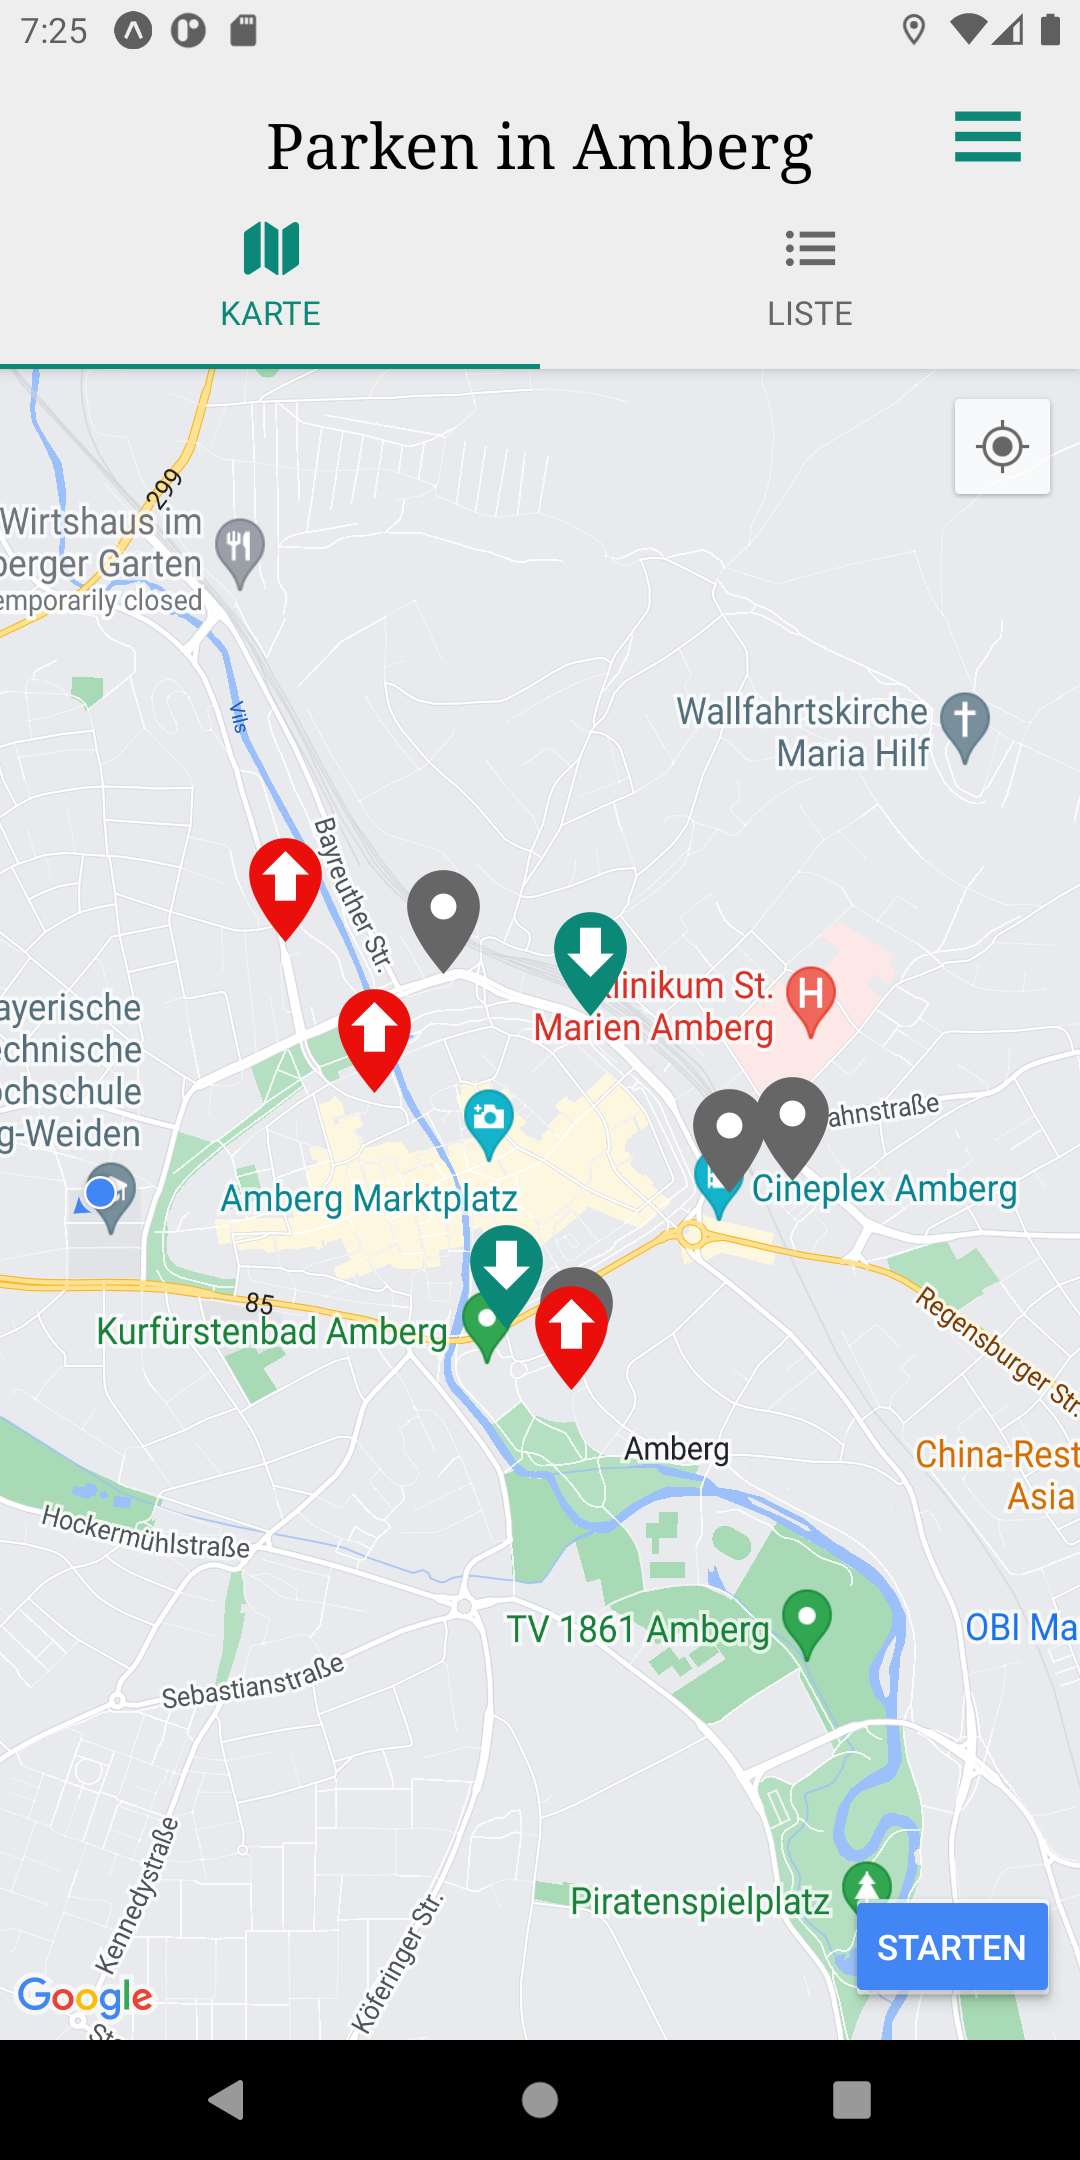
\includegraphics[scale=0.15]{img/map}
	\caption{Ansicht der fertigen App mit der Karte und eingezeichneten Markern}
	\label{fig:map}
\end{wrapfigure}
Die Karte und alle Zusatzfunktionalitäten sind im Ordner \verb|Map| zu finden. Ein erster Prototyp der Karte war sehr schnell implementiert. Hierfür musste nur das Paket react-native-maps installiert werden. Dieses Paket benutzt auf Android-Systemen die Google Maps API und auf iOS-Systemen die Apple Maps API, um eine Karte in der App anzeigen zu können. Wenn dieses Paket mit Expo installiert wird, sind sogar keine API-Keys nötig, um die Karten anzeigen und nutzen zu können. Um nun auch den Standort des Nutzers in der Karte zeigen zu können, wird das Expo-Paket expo-location benötigt \cite{location}. Dieses Paket kann, wenn der Nutzer die Erlaubnis gibt, den Standort des Nutzers herausfinden und in die Karte einzeichnen. Wenn der Nutzer seine Erlaubnis nicht gibt, wird dies auch wahrgenommen und die Funktionalität der App ist dadurch eingeschränkt, da dann nicht mehr herausgefunden werden kann, wie nah der Nutzer einem Parkhaus ist. Um die Parkhäuser in die Karte einzuzeichnen wurde eine Liste aus den statischen Daten erzeugt, welche an das react-native-maps Paket übergeben wird.

Diese Markierungen der Parkhäuser wurden danach noch mit Icons versehen, welche den Trend anzeigen. Diese Icons stammen aus dem react-native-vector-icons Paket \cite{vector-icons}. Die Icons aus diesem Paket werden in der gesamten App verwendet. Ein grüner Marker mit einem Pfeil nach unten bedeutet, dass sich das Parkhaus gerade leert. Ein roter Marker mit einem Pfeil nach oben heißt, dass sich das Parkhaus füllt. Ein grauer Marker bedeutet, dass das Parkhaus einen gleichbleibenden Trend besitzt. Somit kann der Nutzer schon beim Starten der App sofort Informationen zu den Parkhäusern auslesen. Diese Marker mit der Karte sind in \autoref{fig:map} zu sehen. Hier ist der Nutzer als kleiner blauer Punkt mit einem Pfeil in Blickrichtung bei der OTH eingezeichnet.

\begin{wrapfigure}{R}{0.5\textwidth}
	\vspace{-\baselineskip}
	\centering
	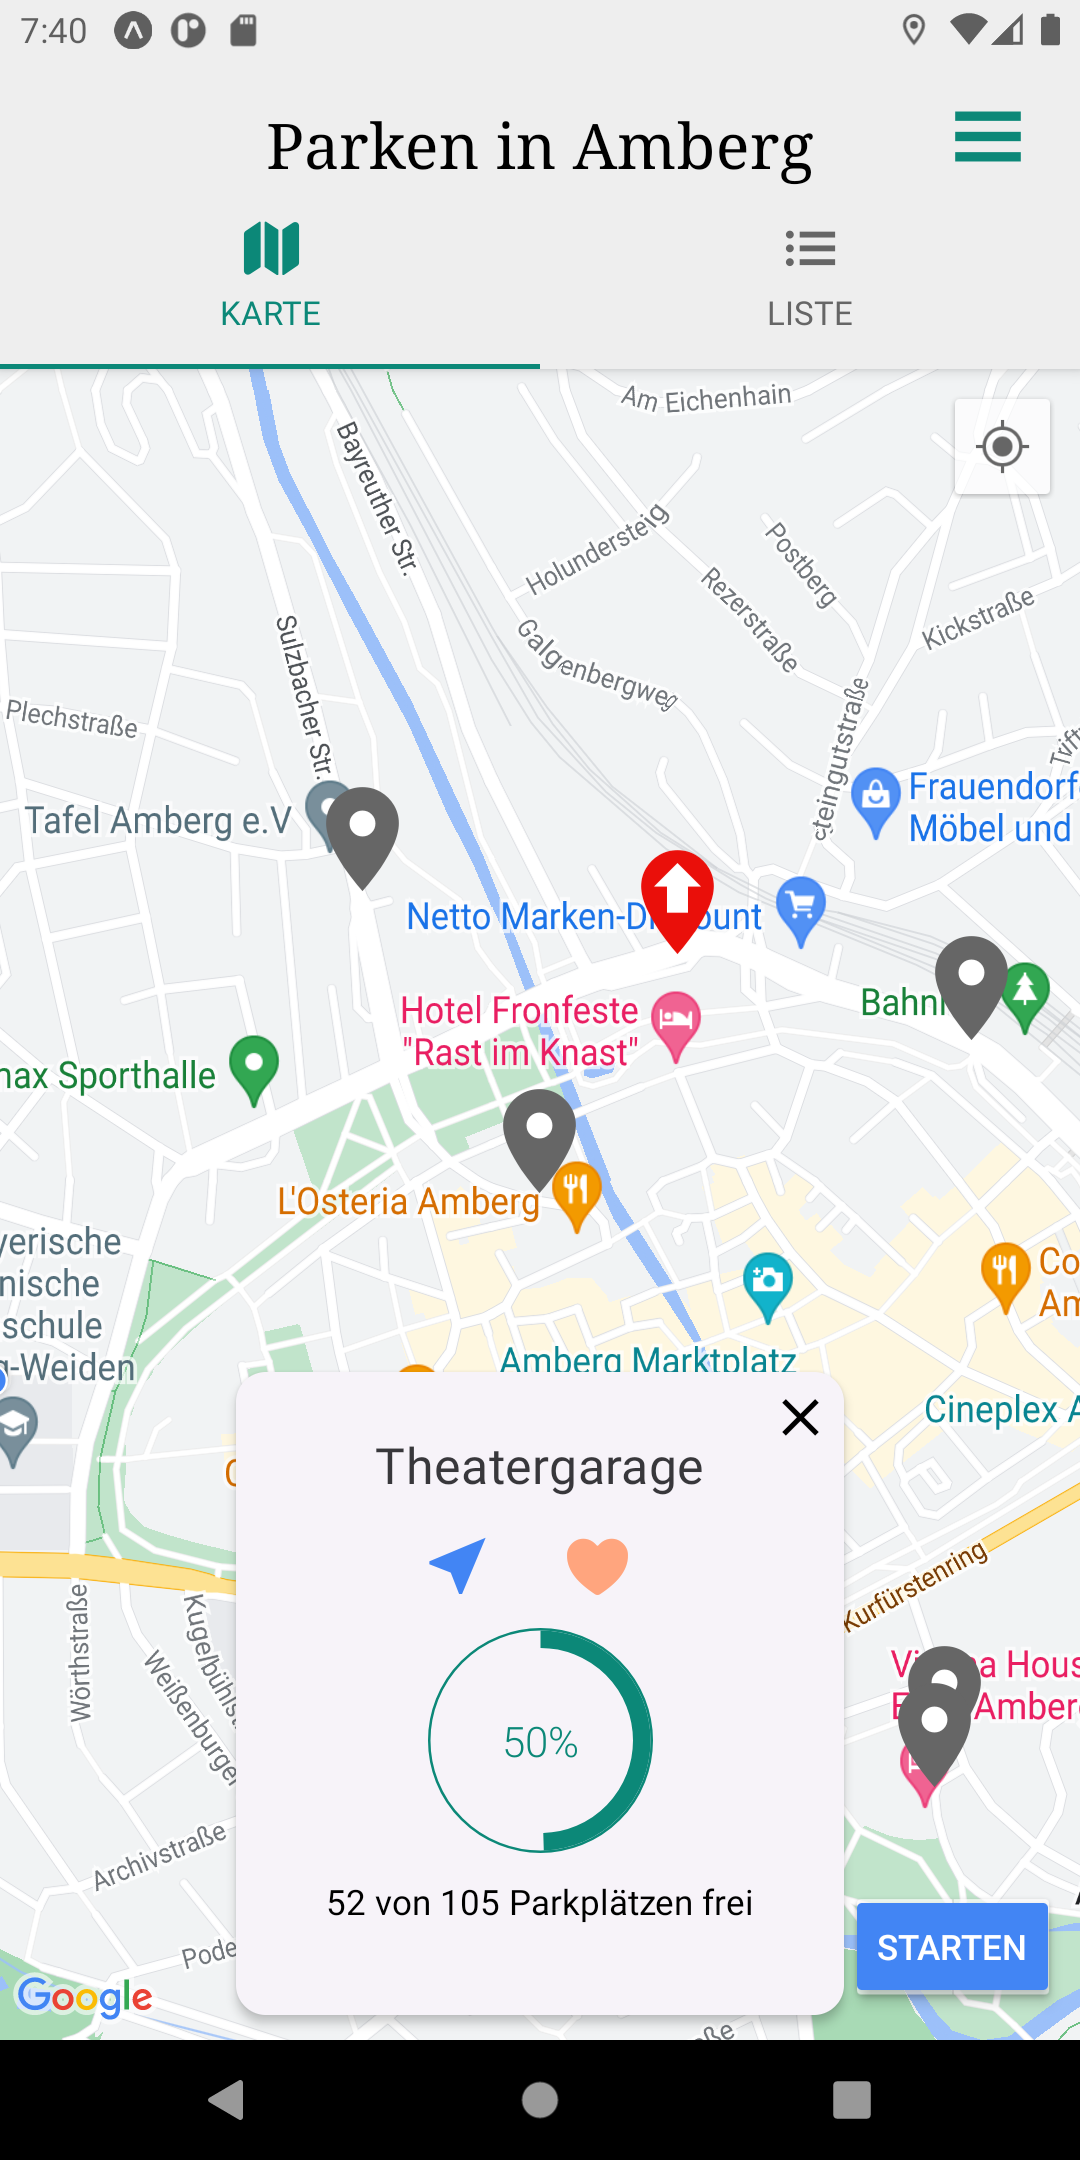
\includegraphics[scale=0.15]{img/detail_map}
	\caption{Detailansicht zum Parkhaus Theatergarage in der Karte}
	\label{fig:detail_map}
\end{wrapfigure}
Durch Anklicken der Marker ist es auch möglich, nähere Informationen zu den einzelnen Parkhäusern zu bekommen. Diese Ansicht ist in \autoref{fig:detail_map} zur Theatergarage zu sehen. Hier wird angezeigt, wie viele Plätze in diesem Parkhaus noch frei sind. Zur besseren Benutzerfreundlichkeit wird dies noch mit einem Fortschritts-Kreis visualisiert, welcher aus dem react-native-progress Paket stammt \cite{progress}. Dieser zeigt den Füllstand des Parkhauses in Prozent an. Je größer der Prozentwert, desto mehr Parkplätze sind frei. Über diesem Kreis sind zwei Icons zu sehen. Der blaue Pfeil links bedeutet die Navigation. Durch Klicken auf dieses Icon wird der Nutzer zu diesem bestimmten Parkhaus navigiert, was später erläutert wird. Das rote Herz links bedeutet, dass dieses Parkhaus vom Nutzer zu den Favoriten hinzugefügt wurde. Wenn das Parkhaus nicht zu den Favoriten gehört, ist das Herz nicht ausgefüllt. Durch einen Klick auf dieses Icon kann der Nutzer zudem das Parkhaus zu den Favoriten hinzufügen oder wieder entfernen.

\begin{wrapfigure}{R}{0.5\textwidth}
	\vspace{-\baselineskip}
	\centering
	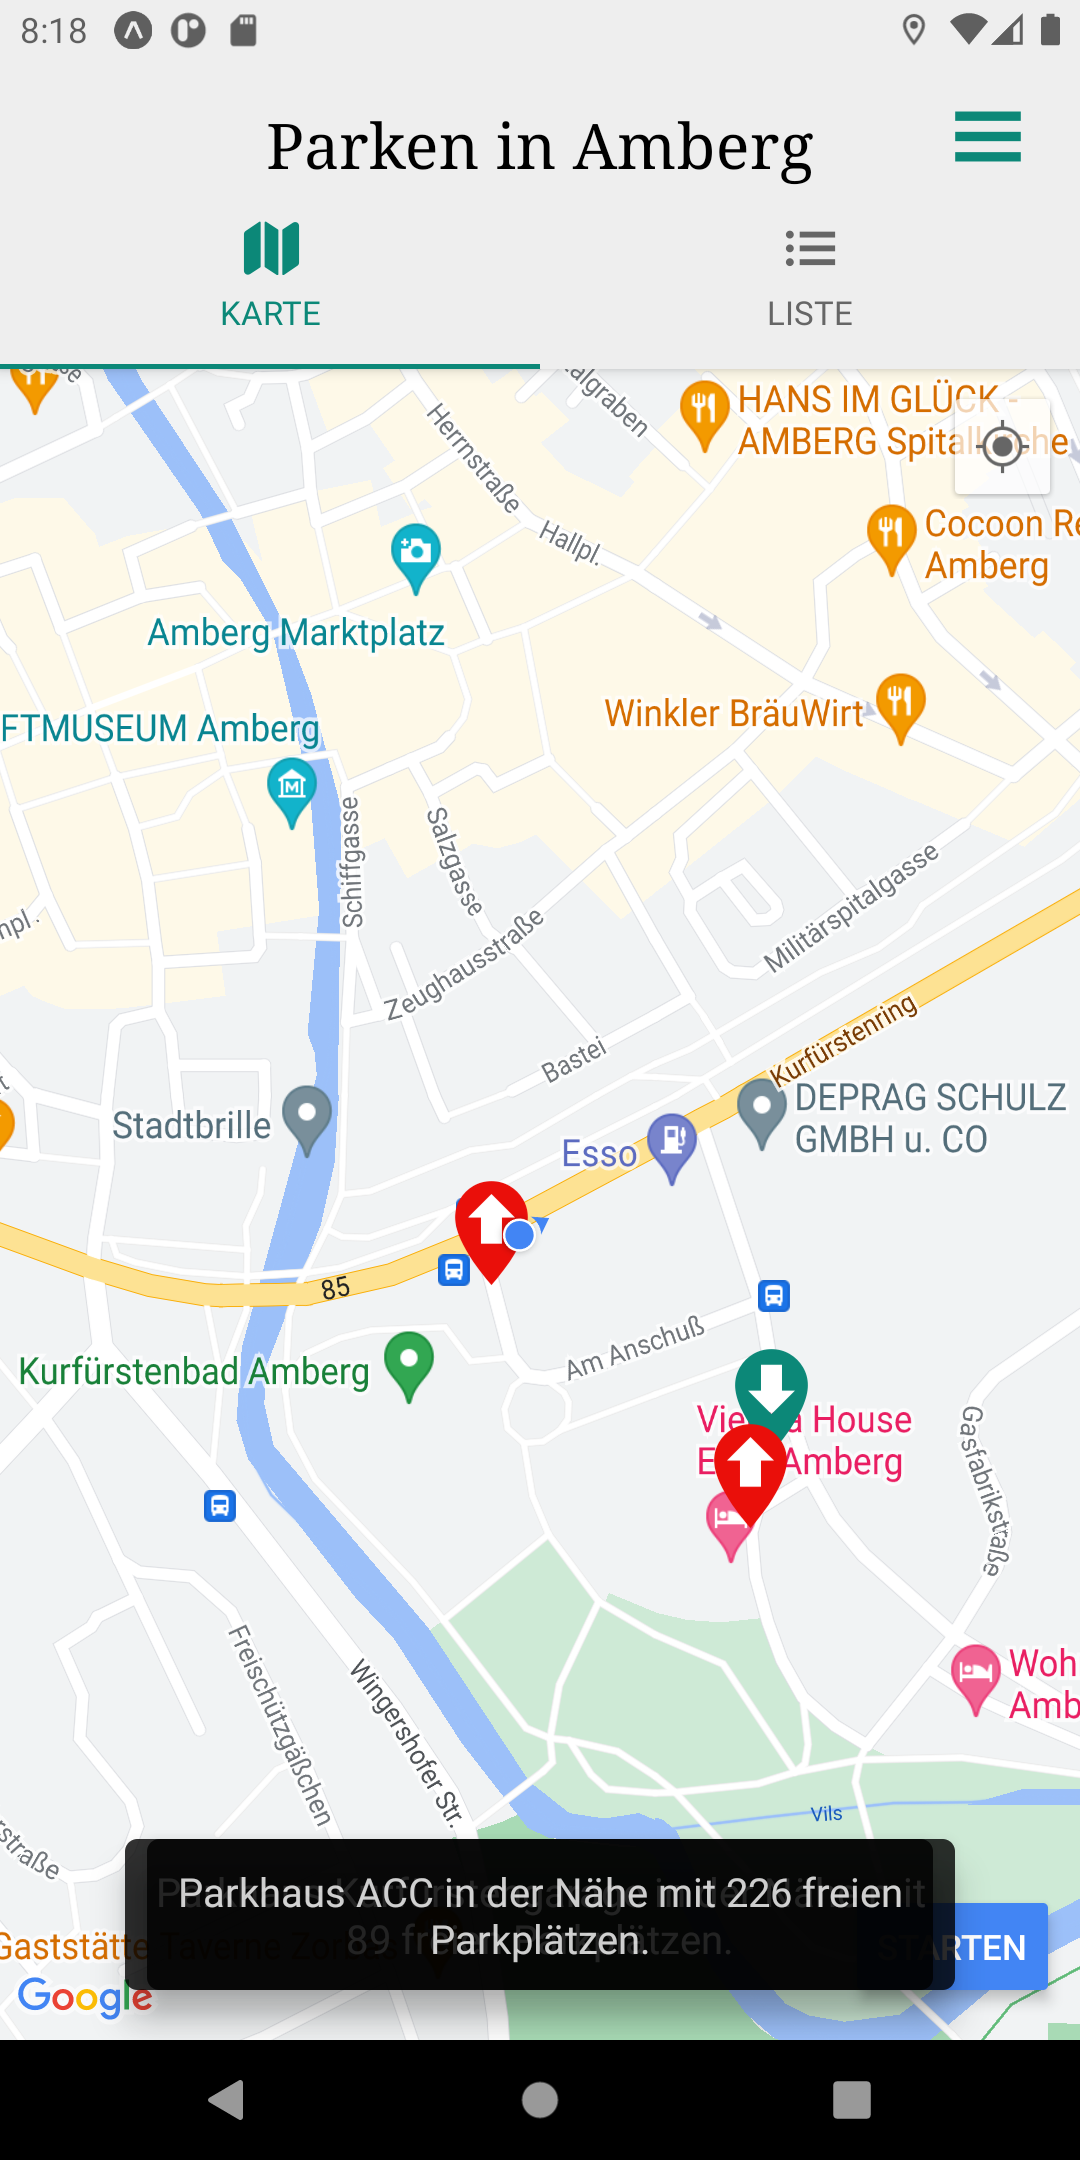
\includegraphics[scale=0.15]{img/Geofencing}
	\caption{Anzeige, dass sich der Nutzer dem Parkhaus ACC nähert, welches 226 freie Parkplätze hat}
	\label{fig:Geofencing}
\end{wrapfigure}
Nachdem die Karte fertig implementiert war, konnten die Anzeigen erstellt werden, dass sich der Nutzer einem Parkhaus nähert. Dies wurde zuerst über Geofencing versucht zu lösen. Geofencing bedeutet, dass die App kreisförmige Bereiche, welche vom Nutzer meist nicht sichtbar sind, um Koordinaten aufspannt. Bei Betreten und Verlassen eines dieser Bereiche wird ein Event mit den Informationen zu dem Bereich, also hier dem Parkhaus, gefeuert. Im expo-location Paket ist standardmäßig Geofencing enthalten. Dies wurde versucht einzufügen, jedoch kam es hierbei zu Problemen. Wenn der Nutzer in mehreren Geofences ist, kann es passieren, dass das Betreten eines anderen Geofences doppelt signalisiert ist. Wie in \url{https://github.com/expo/expo/issues/6283} zu sehen, besteht dieses Problem immer noch und es scheint keinen Fix hierfür zu geben. Deshalb wurde ein eigenes Geofencing implementiert, welches im Ordner \verb|Geofencing| zu finden ist. Dafür musste die Luftlinienentfernung vom Nutzer zu jedem Parkhaus berechnet werden, ob er in der Nähe eines Parkhauses ist. Zur Berechnung der Distanz wurde die bekannte Haversine Formel verwendet \cite{haversine}. Diese kann über die Umwandlung der Winkelkoordinaten Latitude und Longitude ins Bogenmaß den Abstand zwischen zwei Punkten auf einer Kugel sehr genau berechnen.

Um nun den Abstand zu den Parkhäusern zu berechnen, wurde die Position des Nutzers benötigt. Dafür existiert wieder eine Funktion in expo-location, nämlich \verb|startLocationUpdatesAsync|. Diese Funktion schickt kontinuierlich die aktuellen Koordinaten des Nutzers an einen Task, der vorher definiert wurde und im Hintergrund läuft. Der Task nimmt die Koordinaten an und übergibt diese an eine Funktion, welche den Abstand dieser Koordinaten zu jedem Parkhaus berechnet. Falls der Abstand kleiner als 200 Meter ist, wird der Nutzer als ,,in der Nähe des Parkhauses'' angesehen. Falls der Nutzer vorher weiter entfernt als 200 Meter vom Parkhaus war, also außerhalb des ,,Geofences'', erscheint ein Meldung, welchem Parkhaus der Nutzer sich gerade nähert und wie viele freie Parkplätze in diesem aktuell sind. Diese Meldung wird auch über ein text-to-speech Paket vorgelesen \cite{tts}. Die graphische Anzeige der Meldung ist in \autoref{fig:Geofencing} ersichtlich. In welchen Geofences der Nutzer gerade ist wird in einer Liste festgehalten, die später benötigt wird.

\begin{wrapfigure}{R}{0.5\textwidth}
	\vspace{-\baselineskip}
	\centering
	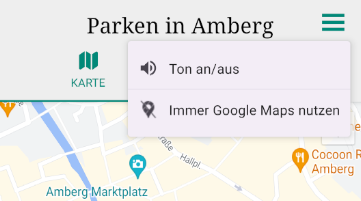
\includegraphics[scale=1]{img/map_settings}
	\caption{Liste an Einstellungen der Karte, welche über ein Burger-Menü verfügbar ist}
	\label{fig:map_settings}
\end{wrapfigure}
Zuletzt wurde die Karte noch mit zwei Einstellungsmöglichkeiten konfigurierbar gemacht. Diese sind über das Burger-Menü rechts oben aufrufbar. Bei Klicken auf das Menü öffnet sich eine Liste mit zwei Einträgen, wie in \autoref{fig:map_settings} sichtbar. Der erste Eintrag steuert, ob die Meldung, dass ein Geofence betreten wurde vorgelesen werden soll oder nicht. Wenn das Icon des Lautsprechers durchgestrichen ist, wird die Vorlese-Funktion ausgeschaltet. Standardmäßig ist diese Funktion angeschaltet. Der zweite Eintrag gibt an, ob bei der Navigation ausschließlich zu Google Maps weitergeleitet werden, oder ob die interne Navigation der App, wenn möglich, genutzt werden soll. Auf diese Navigation wird in \autoref{chap:5} weiter eingegangen. Diese Einstellung ist standardmäßig ausgeschaltet, damit die interne Navigation bevorzugt wird. Die Werte beider Einstellungen werden zudem ebenfalls in async-storage gespeichert, damit der Nutzer die App nicht bei jedem Öffnen neu konfigurieren muss.

Damit ist die Implementierung der Karte abgeschlossen. Im Folgenden wird die Funktionalität und Umsetzung der Liste beschrieben.

  \chapter{Implementierung der Liste}
\label{chap:4}

\begin{wrapfigure}{R}{0.5\textwidth}
	\vspace{-\baselineskip}
	\centering
	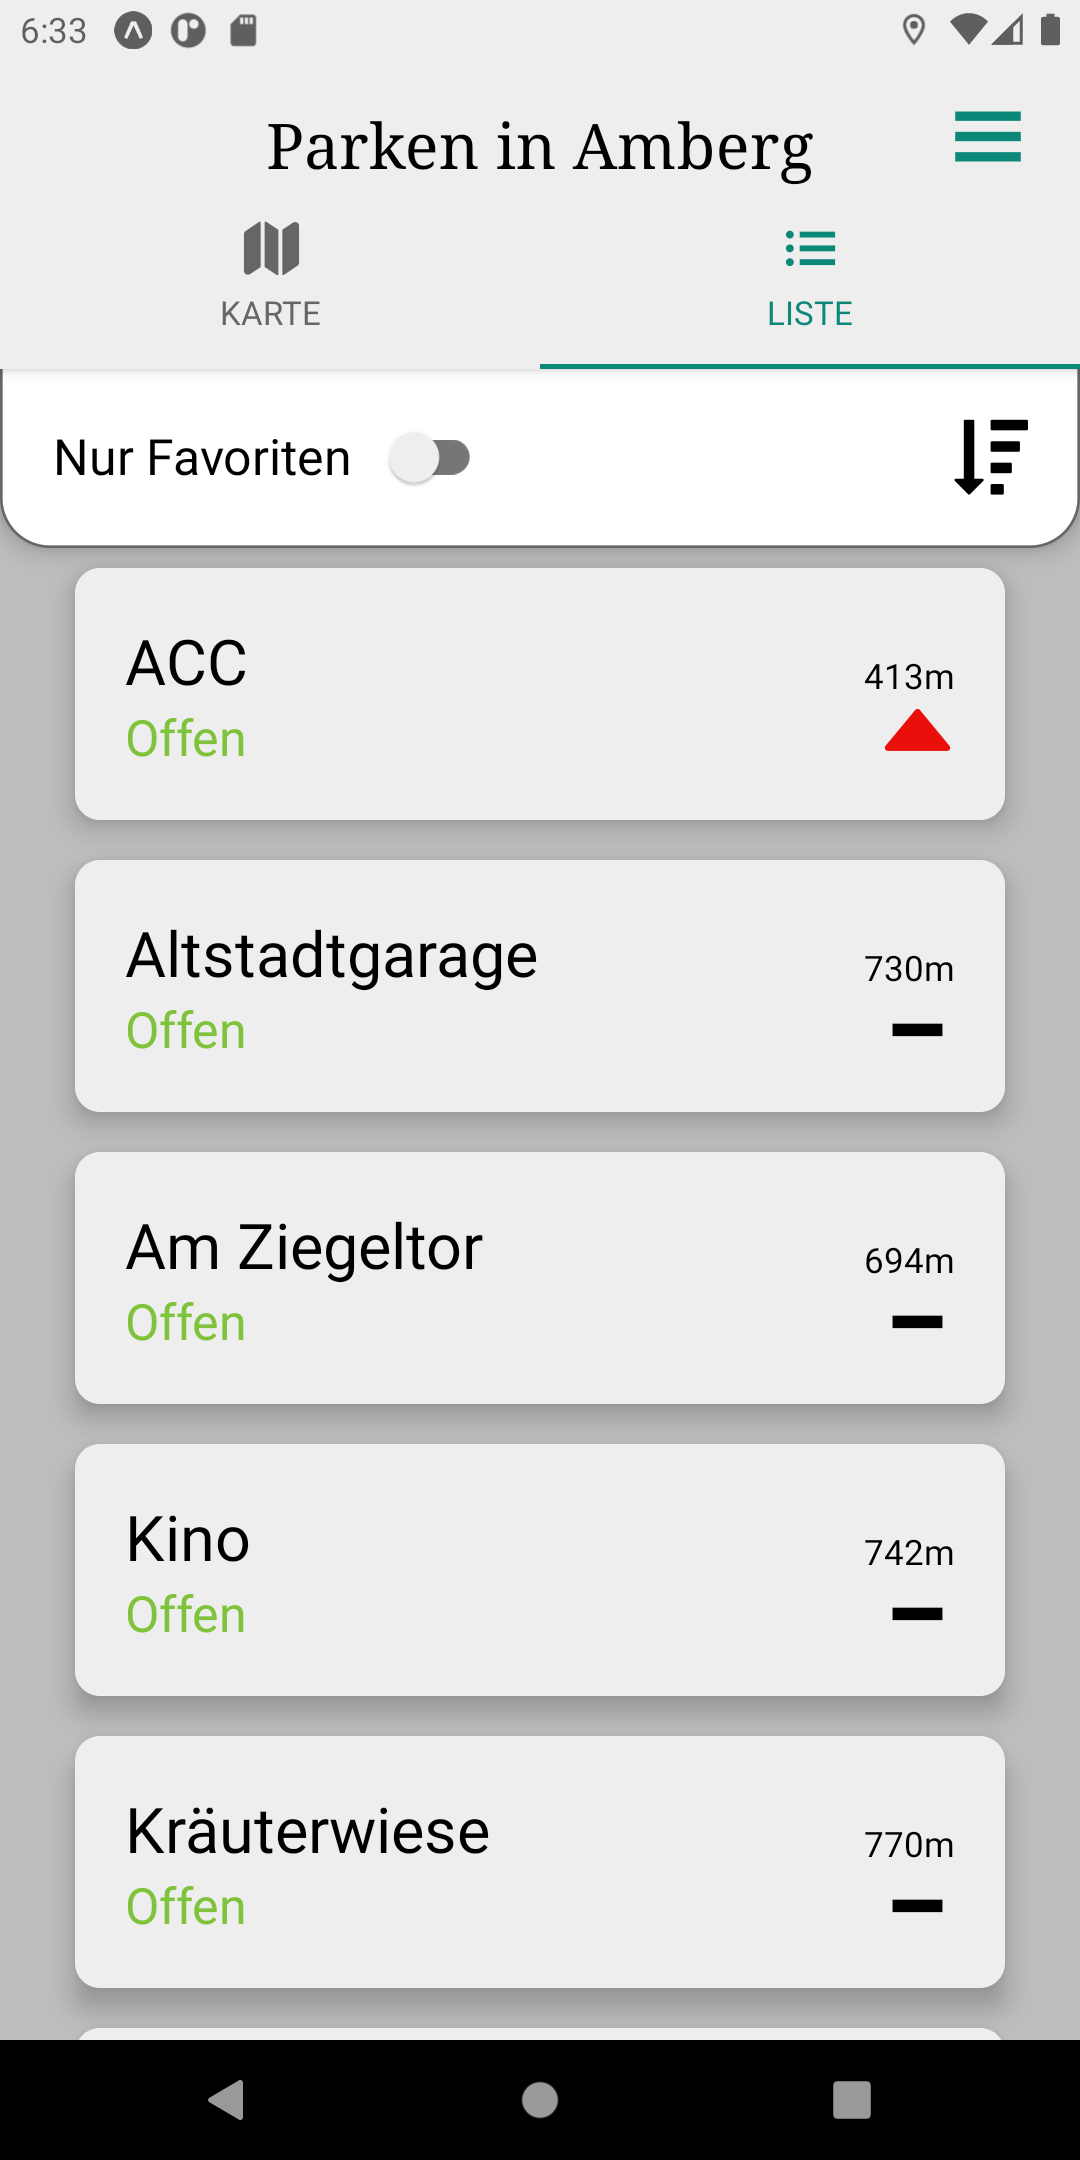
\includegraphics[scale=0.15]{img/list}
	\caption{Ansicht des Listen-Tabs mit der alphabetisch geordneten Liste an Parkhäusern}
	\label{fig:list}
\end{wrapfigure}
Alle Komponenten, aus denen die Liste besteht, sind im Ordner \verb|ParkingList| enthalten. Für die Liste selbst wird die FlatList-Komponente, welche standardmäßig im react-native Framework enthalten ist, verwendet. Dafür wird durch eine Funktion ein Array aus den dynamischen und statischen Daten erzeugt, welche an die FlatList-Komponente zur Anzeige übergeben wird. Die Erzeugung und Anzeige des Arrays ist in der Datei \verb|ParkingList.tsx| zu finden. Die anzuzeigenden Daten sind zum einen der Name des Parkhauses zur Identifizierung. Darunter wird dargestellt, ob das Parkhaus geöffnet oder geschlossen ist. Wenn das Parkhaus offen ist, wird dies in grüner Schrift angezeigt, geschlossen wird dagegen rot geschrieben. Da alle Parkhäuser 24 Stunden offen sind, sollte ein geschlossenes Parkhaus nur bei Wartungsarbeiten und Störungen auftreten. Rechts daneben wird die Entfernung des Nutzers zu diesem spezifischen Parkhaus in Metern angezeigt. Die Position des Nutzers wird wieder über dieselbe Methode erlangt, wie in \autoref{chap:3} für das Geofencing. Über die Haversine Distanz wird wieder die Entfernung zu den Koordinaten der Parkhäuser berechnet und dann angezeigt. Dies wird bei jeder Positionsänderung des Nutzers durchgeführt, damit die Entfernungen immer aktuell sind. Darunter wird noch der Trend des Parkhauses über Icons symbolisiert. Ein grüner Pfeil nach unten signalisiert, dass sich das Parkhaus leert, ein roter Pfeil nach über bedeutet ein sich füllendes Parkhaus und ein schwarzer Balken zeigt einen gleichbleibenden Trend an, wie mit den Markern der Karte.

\begin{wrapfigure}{R}{0.5\textwidth}
	\vspace{-\baselineskip}
	\centering
	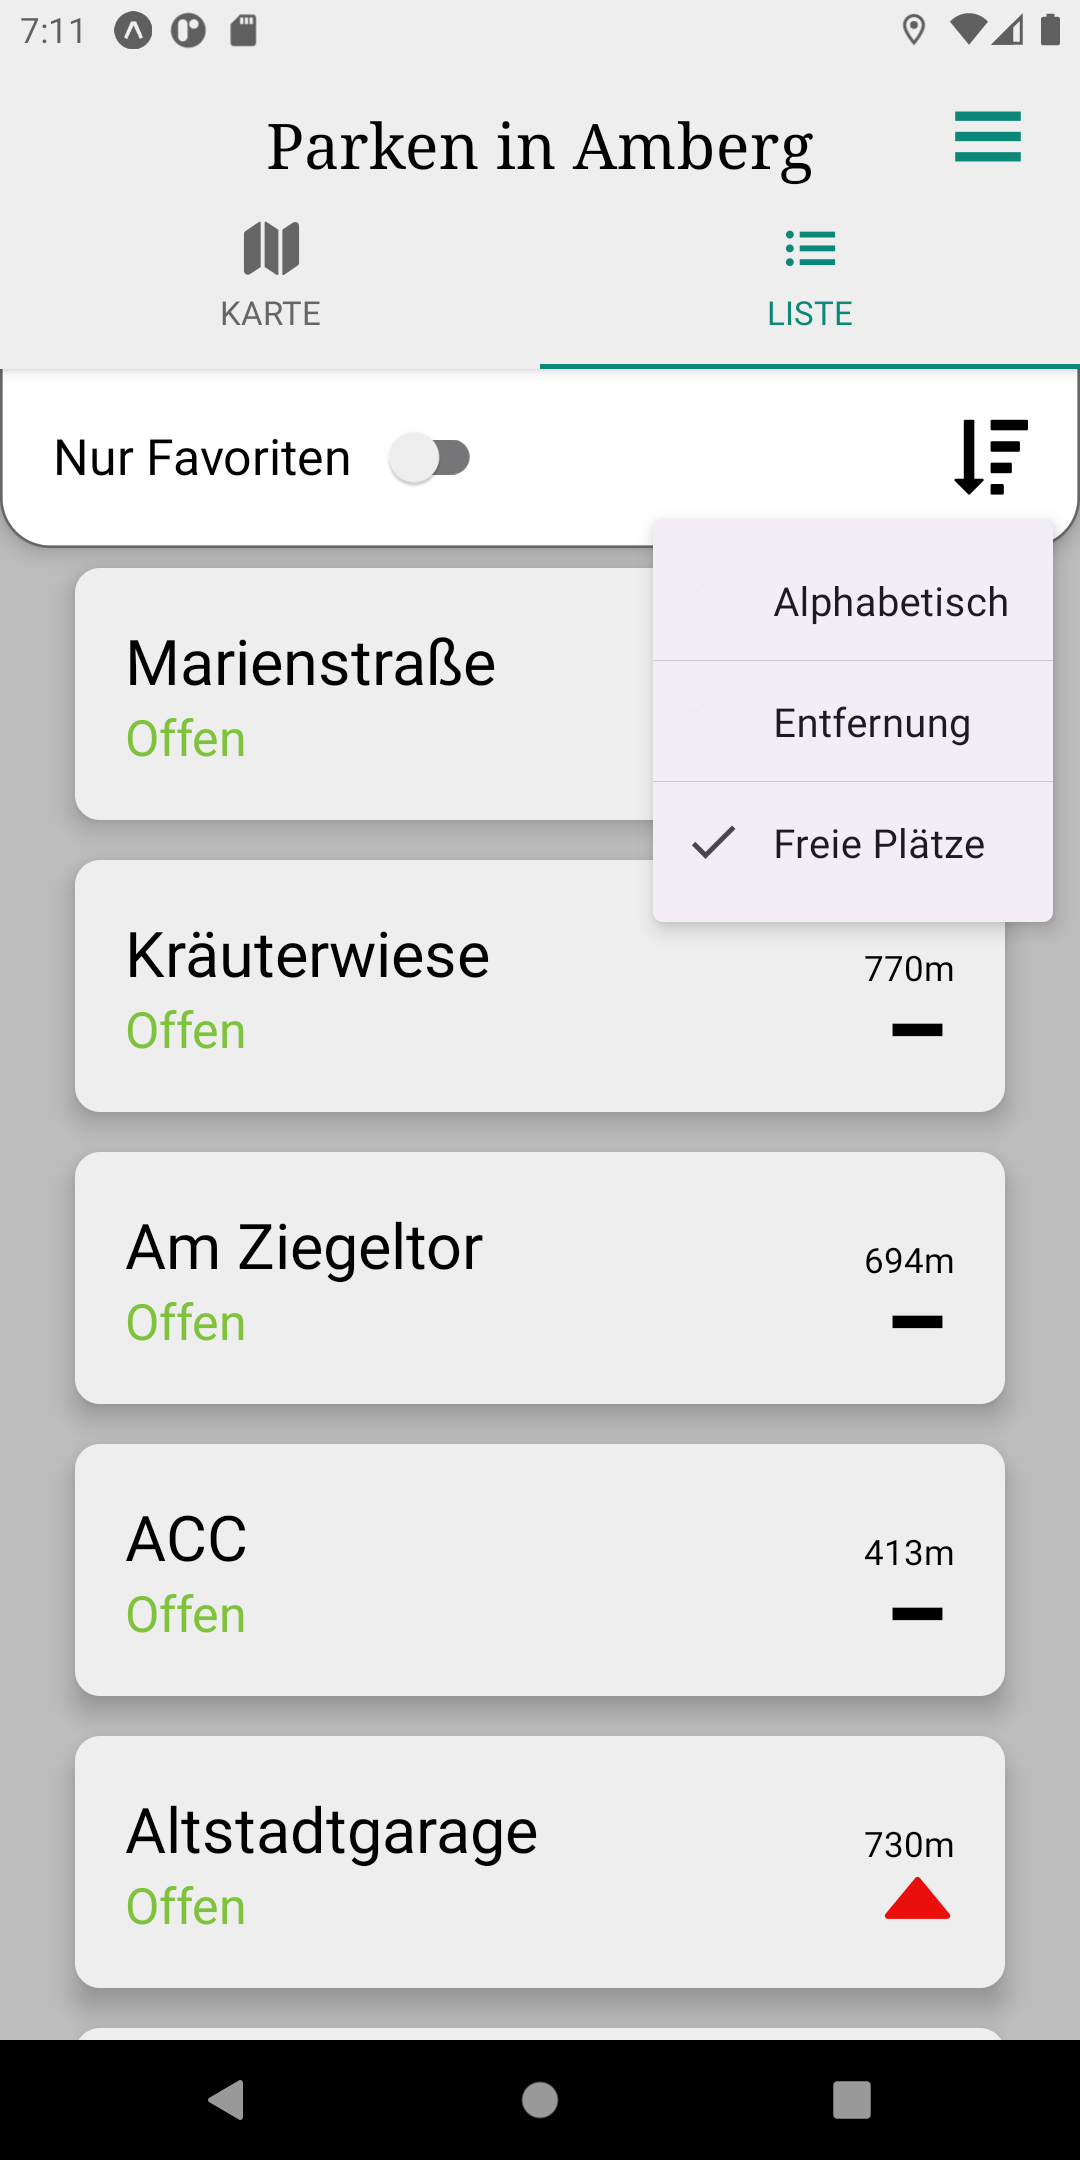
\includegraphics[scale=0.15]{img/sorting}
	\caption{Aufruf des Menüs zum Sortieren der Liste}
	\label{fig:sorting}
\end{wrapfigure}
Diese Liste kann zudem auch konfiguriert werden. Dafür ist zu einen links oben der Liste ein Schalter vorhanden, für den die Switch-Komponente von react-native benutzt wurde, mit der Beschreibung ,,Nur Favoriten''. Wenn dieser Schalter gesetzt ist, werden nur die Parkhäuser angezeigt, welche als Favorit markiert wurden, also bei welchen das rote Herz ausgefüllt ist, wie in \autoref{fig:detail_map} zu sehen ist. Zudem ist rechts oben ein Sortier-Icon zu sehen. Wenn auf dieses Icon geklickt wird öffnet sich eine Liste an Sortiermöglichkeiten, wobei dieses Menü wieder aus dem Paket react-native-paper stammt. Diese Liste ist in \autoref{fig:sorting} ersichtlich. Es gibt drei Sortiermöglichkeiten. Die erste sortiert alphabetisch nach den Namen der Parkhäuser. Die zweite sortiert aufsteigend nach den Entfernungen, sodass das näheste Parkhaus ganz oben steht. Da die Entfernungen bei jeder Positionsänderung des Nutzers neu berechnet werden, wird auch die Liste neu sortiert, wenn ein Parkhaus nach einer Positionsänderung näher als das andere am Nutzer ist. Somit ist das näheste Parkhaus immer oben. Die letzte Möglichkeit sortiert absteigend nach den freien Plätzen, also je mehr Parkplätze in einem Parkhaus frei sind, desto weiter oben ist es in der Liste.

Da es nicht möglich war, alle Daten zu den Parkhäusern in der Liste anzuzeigen, mussten Detail-Fenster erzeugt werden, die nähere Informationen zu den Parkhäusern darstellen. Diese Detail-Fenster sind über Anklicken des zugehörigen Listeneintrags aufrufbar. Um zwischen der Liste und den verschiedenen Detail-Fenstern der Parkhäuser navigieren zu können, wurde das Paket React Navigation benutzt. Dieses ermöglicht das Aufrufen von Fenstern über die Screen-Komponente. Diese Fenster besitzen einen Zurück-Knopf, wie in \autoref{fig:details1} ersichtlich, mit dem zum letzten Fenster, also der Liste, zurück navigiert werden kann. Das Detail-Fenster besitzt zudem auf die Navigations- und Favoriten-Icons der Karte, welche hier dieselbe Funktion besitzen. Durch Drücken des Navigations-Icons wird der Nutzer hier jedoch entweder zur Karte für die interne Navigation, oder direkt zu Google Maps weitergeleitet.
\newpage

\begin{wrapfigure}{r}{0.5\textwidth}
	\vspace{-\baselineskip}
	\centering
	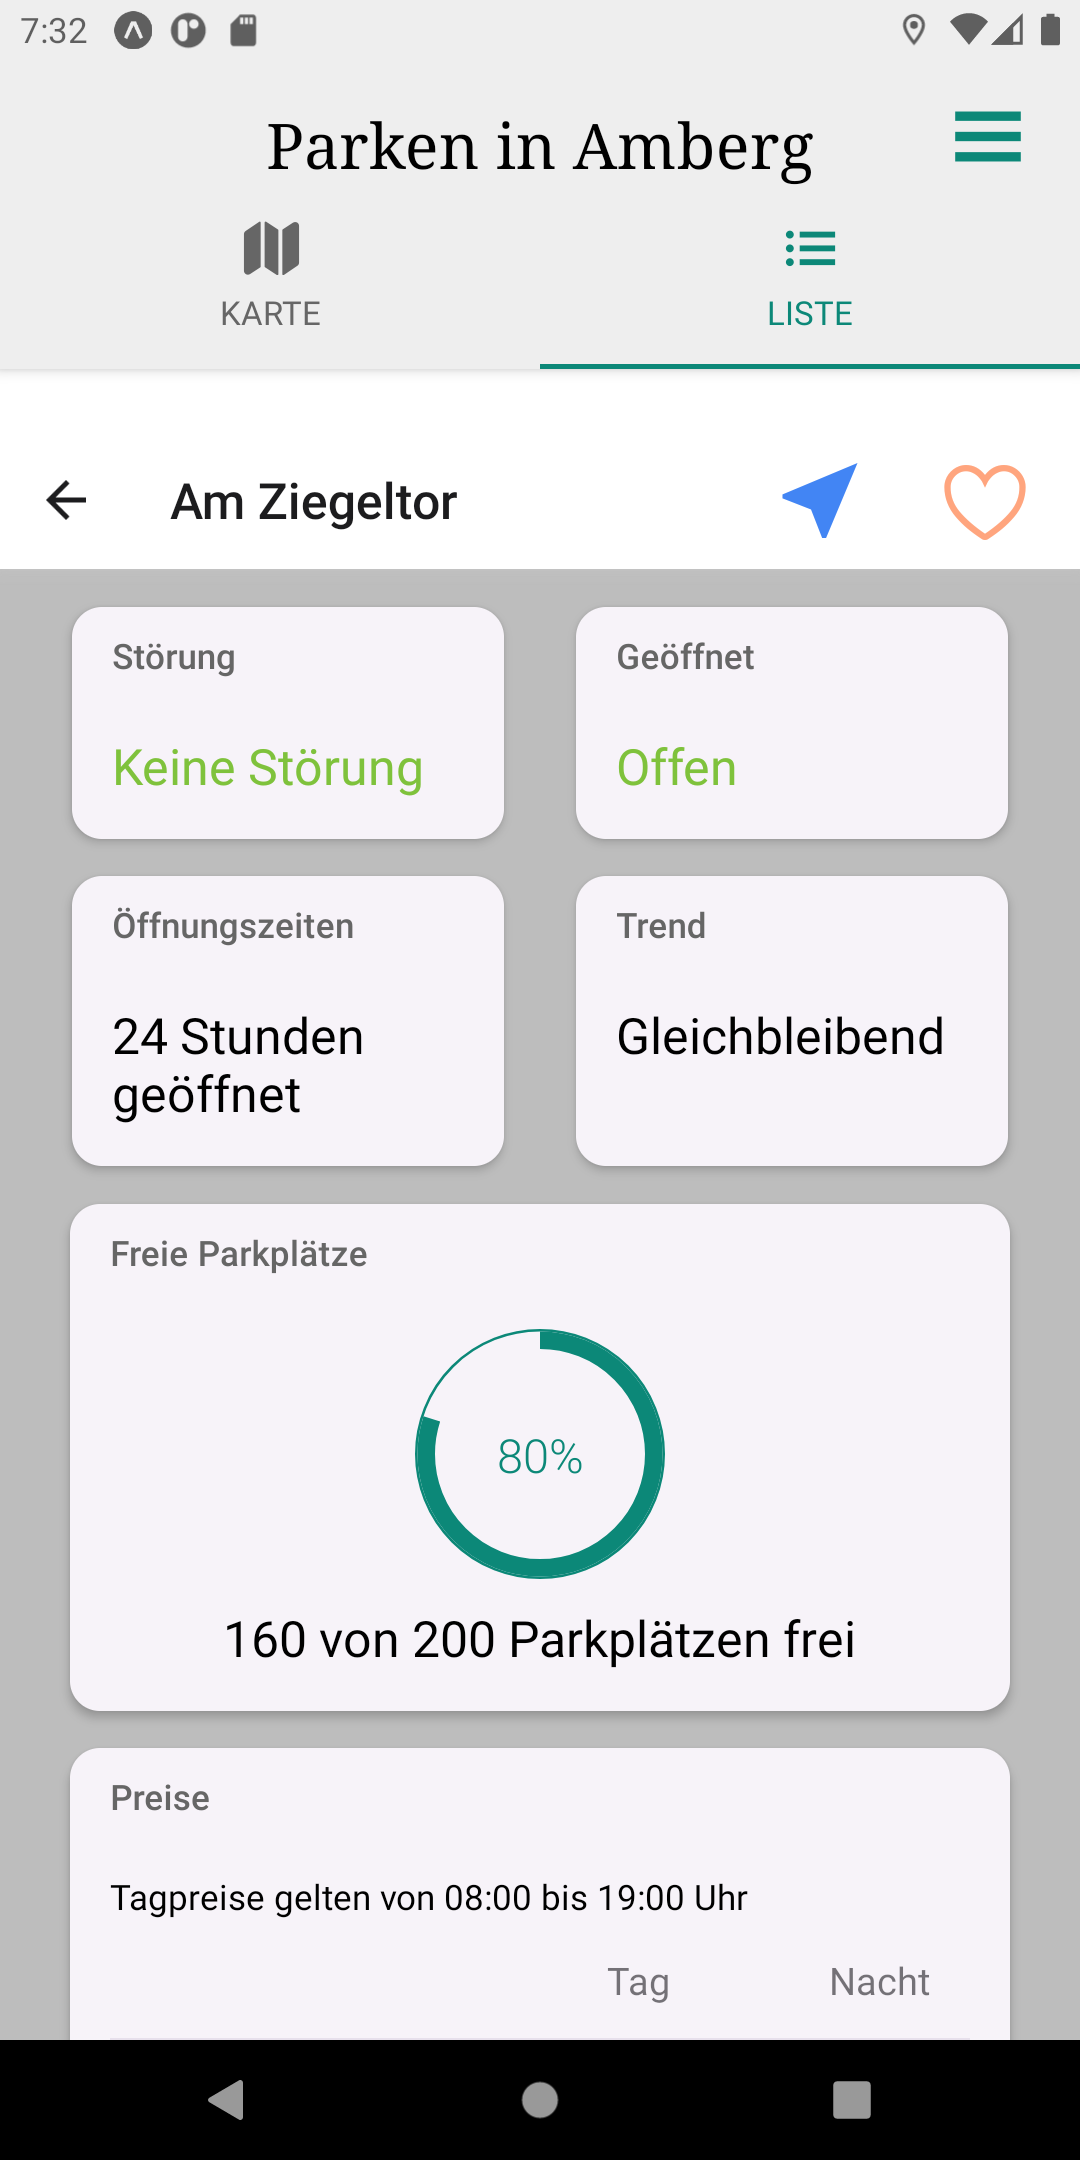
\includegraphics[scale=0.13]{img/details1}
	\caption{Erster Teil des Detail-Fensters zum Parkhaus am Ziegeltor}
	\label{fig:details1}
\end{wrapfigure}
Zur Anzeige der restlichen Informationen des Parkhauses wurde wieder das react-native-paper Paket benutzt. Hier bestehen die weißen Kasten, aus denen sich das Detail-Fenster zusammensetzt, aus der Card Komponente. Zuerst wird durch rote oder grüne Schrift gezeigt, ob es in diesem Parkhaus gerade eine Störung gibt oder nicht und ob das Parkhaus offen ist. Danach werden die Öffnungszeiten angeschrieben und der Trend nochmals schriftlich gezeigt. Darunter wird die Anzahl der freien Parkplätze auf dieselbe Weise wie in der Karte gezeigt.

\begin{wrapfigure}{r}{0.5\textwidth}
	\vspace{-\baselineskip}
	\centering
	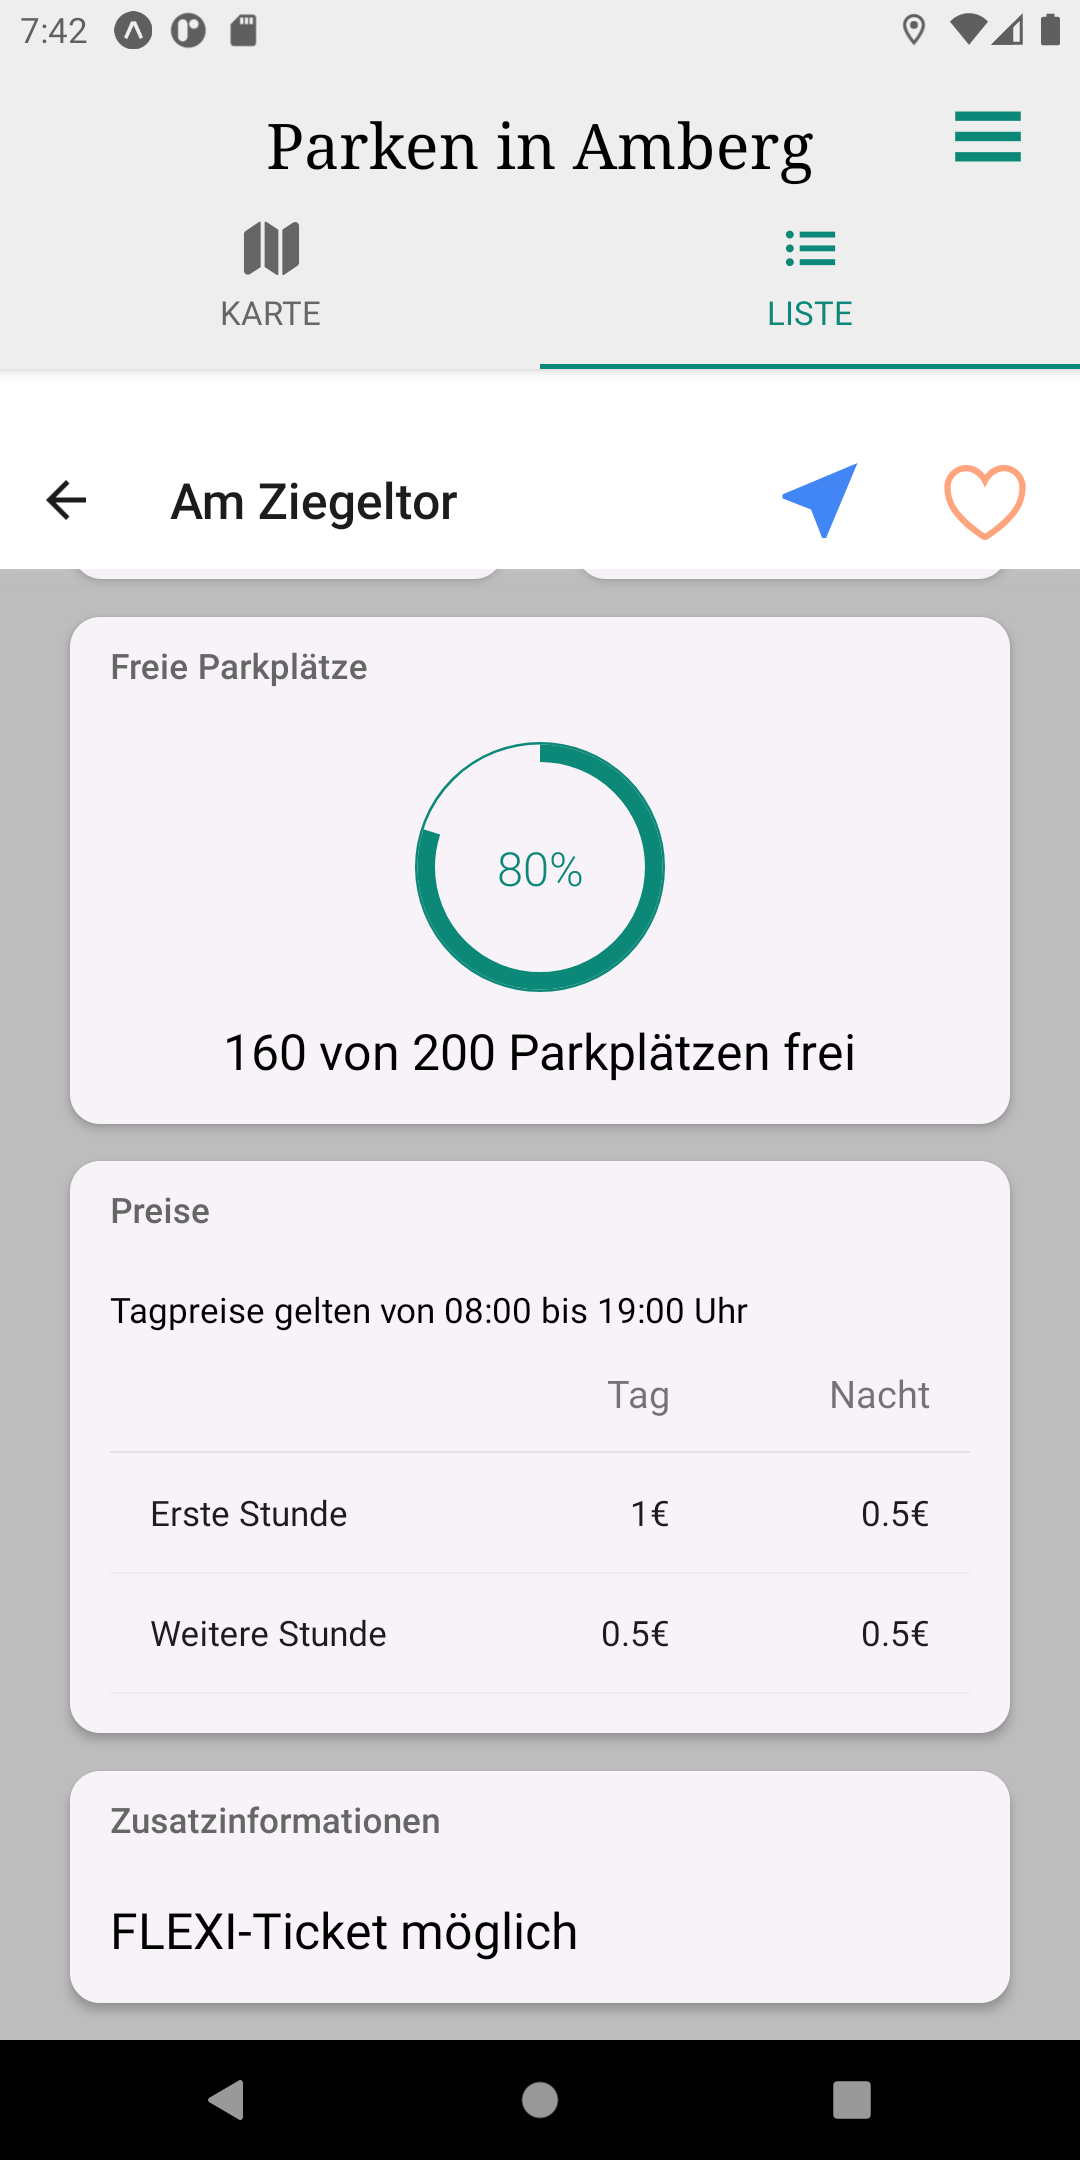
\includegraphics[scale=0.12]{img/details2}
	\caption{Zweiter Teil des Detail-Fensters zum Parkhaus am Ziegeltor}
	\label{fig:details2}
\end{wrapfigure}
Unter den freien Parkplätzen sind die Preise dargestellt. Wenn eine Unterscheidung in Tag- und Nachtpreise nötig ist, wie beim Parkhaus am Ziegeltor, werden diese Preise als Tabelle gezeigt, wobei hier jeweils der Preis für die erste und die weiteren Stunden eingetragen ist. Die Tabelle besteht aus der DataTable-Komponente des react-native-paper Pakets. Unter den Preisen sind nur noch die Zusatzinformationen der statischen Daten zu sehen. Damit werden alle verfügbaren Daten angezeigt und dem Nutzer übersichtlich und benutzerfreundlich dargestellt.

Damit sind alle Komponenten und Funktionalitäten der Liste beschrieben worden. Um die Funktionsweise und den Effekt der Navigationsknöpfe in der Karte und in den Detail-Fenstern der Parkhäuser besser verstehen zu können, wird im nächsten Kapitel auf die interne Pseudo-Navigation eingegangen, welche für diese App erstellt wurde und wie diese Navigation reagiert, wenn kein Weg zum Parkhaus gefunden werden kann.


  \chapter{Umsetzung einer Pseudo-Navigation}
\label{chap:5}

\begin{wrapfigure}{R}{0.6\textwidth}
	\vspace{-\baselineskip}
	\centering
	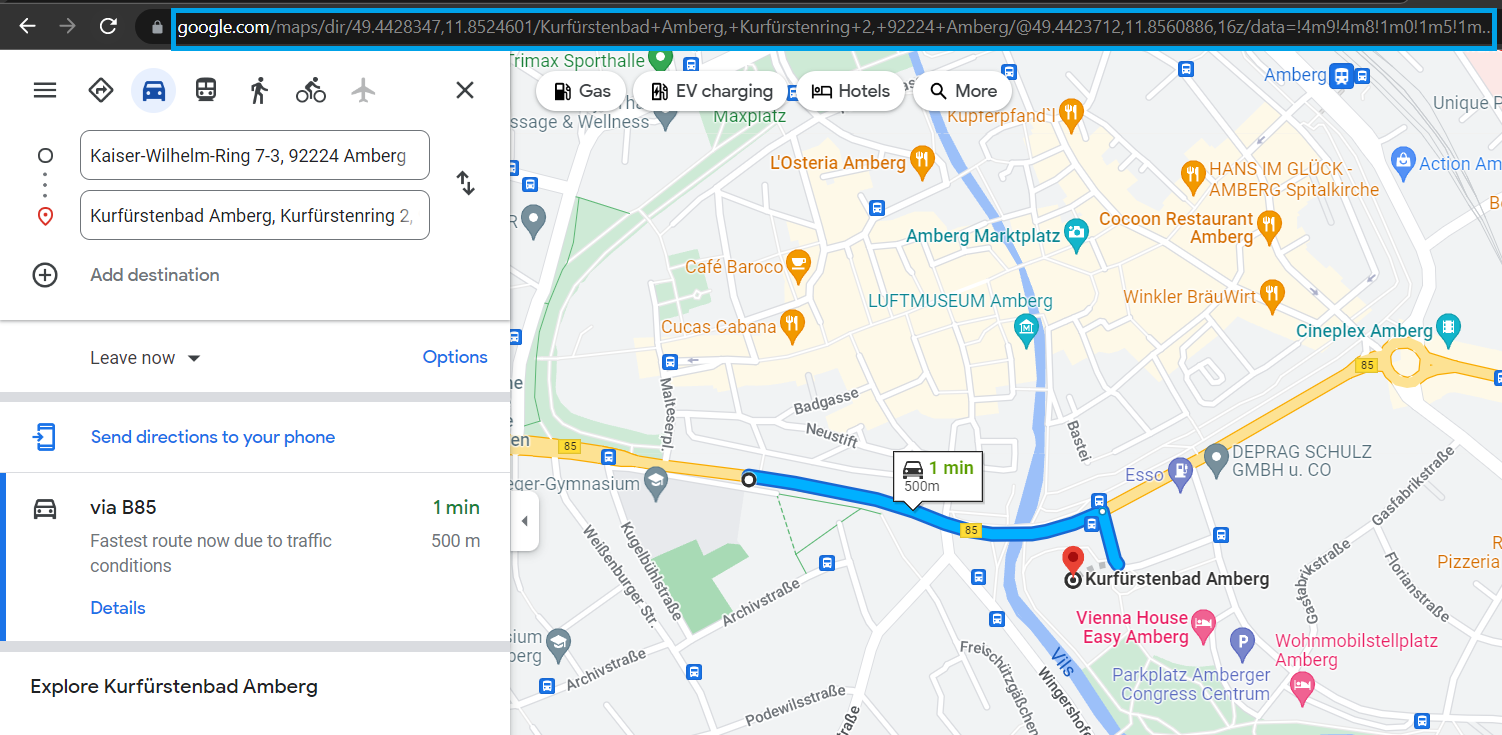
\includegraphics[scale=0.3]{img/path}
	\caption{Berechnung des Wegs zum nähesten Parkhaus von einem Punkt im Altstadtring mit markierter URL}
	\label{fig:path}
\end{wrapfigure}
Die Funktionen und Dateien der Navigation sind im Ordner \verb|Navigation| angesiedelt. Zentral für die Navigation ist die Datei \verb|findCorrectGpxFile.ts|. Diese Datei enthält Funktionen, welche eine Liste aus 48 GPX-Dateien analysiert und die richtige für die Navigation auswählt. Diese GPX-Dateien wurden per Hand erstellt, indem ein Punkt im Altstadtring auf der Karte ausgewählt wurde. Von diesem Punkt aus, wurde durch die App das näheste Parkhaus über Luftlinie, also wieder Haversine Distanz, berechnet. Mit diesen Daten wurde ein Pfad in Google Maps zu diesem Parkhaus berechnet, wie in \autoref{fig:path} zu sehen ist. Die Informationen dieses Wegs werden in die URL geschrieben. Mithilfe eines Parsers können diese Informationen in eine GPX-Datei umgewandelt werden, die wiederum in die Karte der App durch das react-native-maps Paket über die Polyline-Komponente eingezeichnet werden können. Ein möglicher Parser ist die ,,Maps to GPX Converter''-Webseite, welche den Google Maps Link annimmt und daraus eine GPX-Datei des Pfades erzeugt. Mit dieser Methode wurde einmal um den ganzen Altstadtring in 100 Meter Abständen der Weg zum nähesten Parkhaus berechnet. Das Ergebnis sind die oben erwähnten 48 GPX-Dateien, welche zudem noch in TypeScript-Dateien umgewandelt werden mussten, um diese für react-native verfügbar zu machen.

Um nun die richtige GPX-Datei zu finden, muss der Funktion \verb|findCorrectGpxFile| in der gleichnamigen Datei nur die Zielkoordinaten, also die Koordinaten des Parkhauses, zu dem navigiert werden soll, übergeben werden. Wenn diese Koordinaten 0 sind, wird automatisch zum nähesten Parkhaus navigiert. Die Suche nach der Datei zum nähesten Parkhaus läuft dann folgendermaßen ab: Zuerst erfrägt die Funktion die aktuelle Position des Nutzer. Mit dieser Position wird die Entfernung zu allen Anfangspunkten der 48 GPX-Dateien über die Haversine Distanz berechnet. Wenn der Nutzer mehr als 100 Meter von allen Startpunkten der Dateien entfernt ist, ist die Navigation zu ungenau und der Nutzer wird zu Google Maps weitergeleitet. Falls es Startpunkte gibt, die weniger als 100 Meter entfernt sind, wird die GPX-Datei mit dem nähesten Startpunkt genommen. Diese GPX-Datei wird dann an die \verb|Directions.tsx|-Komponente im Ordner \verb|Map| übergeben, damit diese den Pfad in die Karte einzeichnet, was in \autoref{fig:navigation} gezeigt wird.

\begin{wrapfigure}{R}{0.5\textwidth}
	\vspace{-\baselineskip}
	\centering
	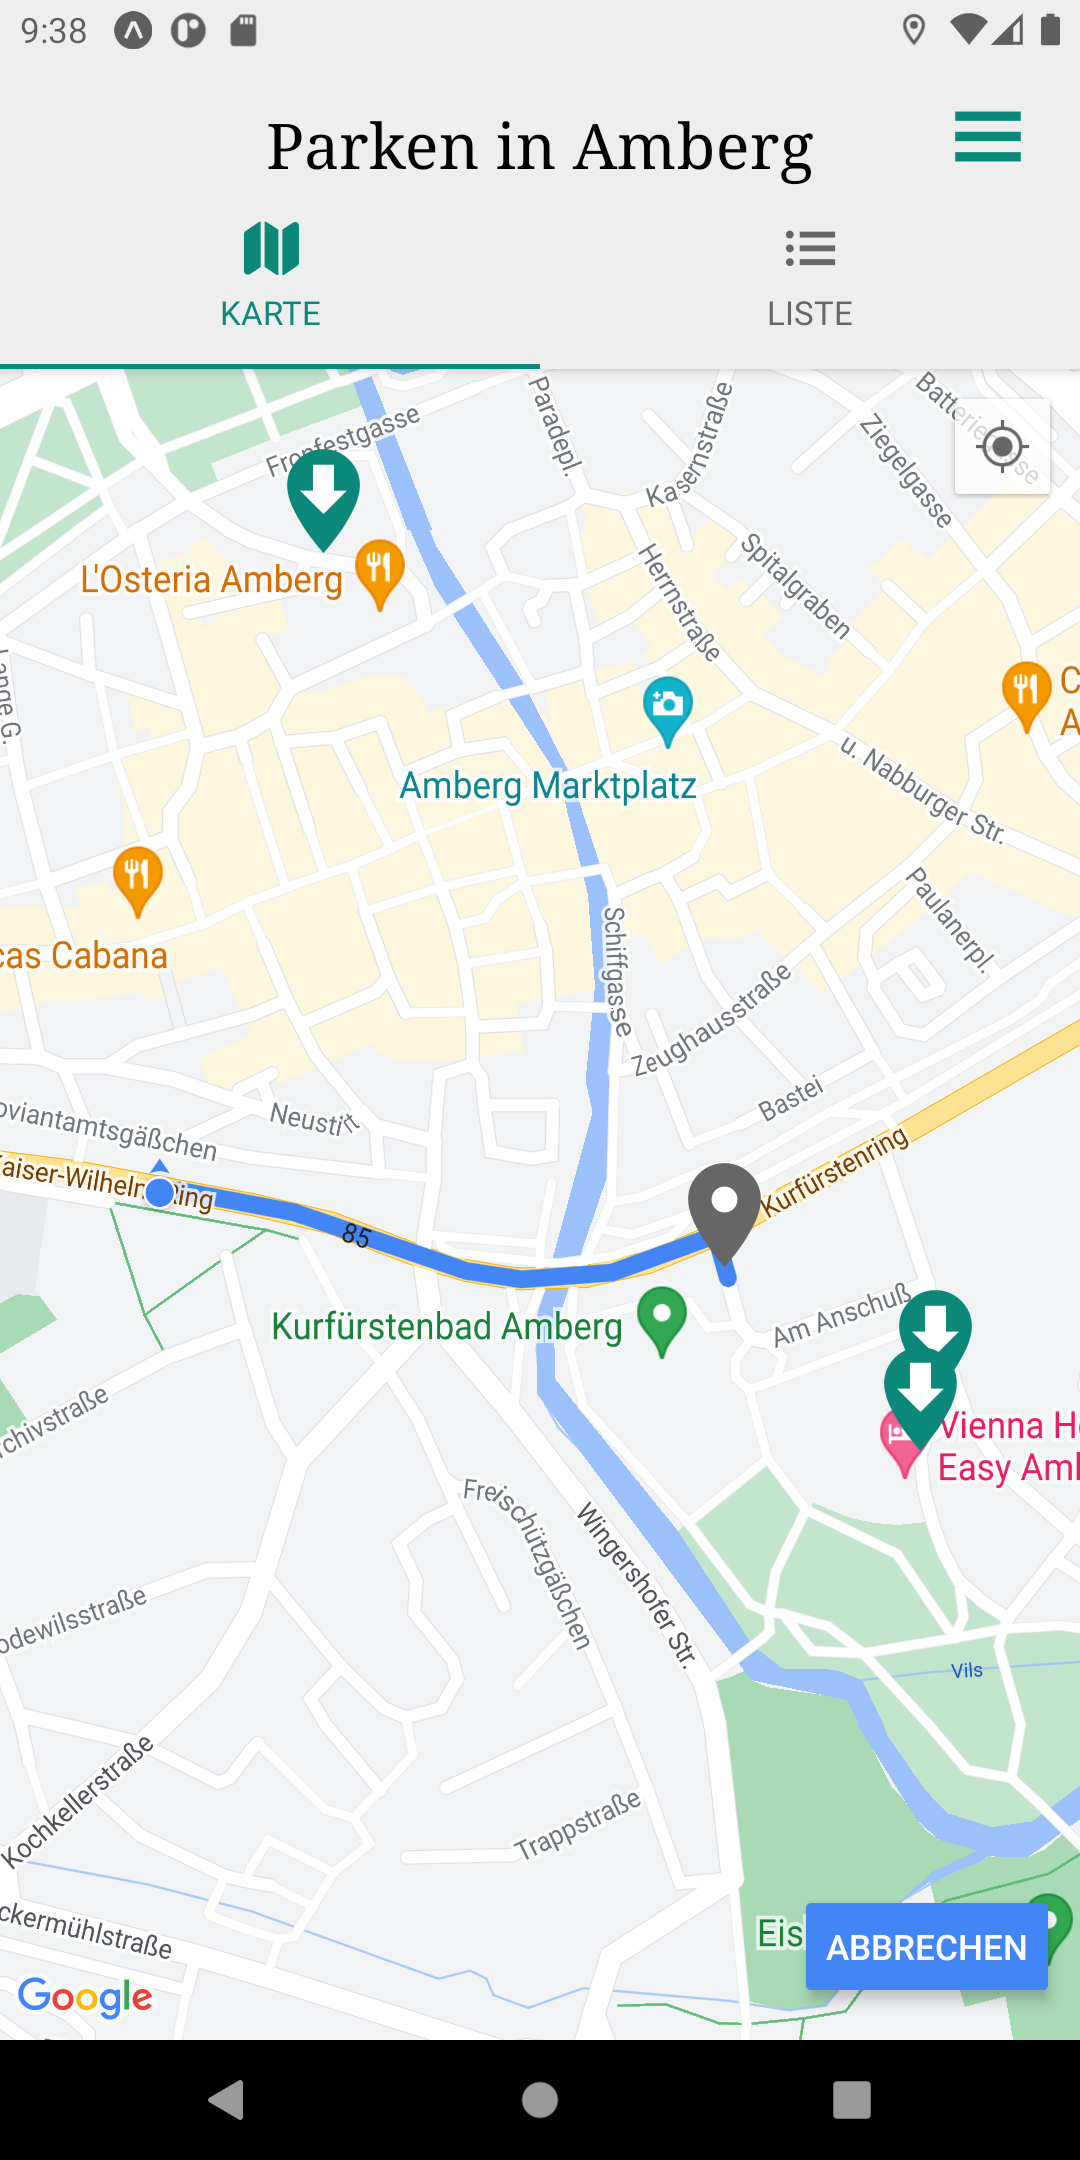
\includegraphics[scale=0.15]{img/navigation}
	\caption{Interne Navigation zum Kurfürstenbad über Einzeichnen der Daten einer GPX-Datei}
	\label{fig:navigation}
\end{wrapfigure}
Falls nun ein bestimmtes Parkhaus gefunden werden soll, wird wieder zuerst die Position des Nutzers erfragt. Danach werden die Entfernungen der Startpunkte der GPX-Dateien berechnet. Hier werden alle GPX-Dateien in einem Array gespeichert, deren Startpunkt weniger als 50 Meter vom Nutzer entfernt sind, da diese Navigation genauer sein soll. Dieses Array wird nun für die Endpunkte durchgegangen. Zu jedem Kandidaten der Dateien wird die Entfernung des Endpunkts zur gewünschten Zielkoordinate des Parkhauses berechnet. Falls ein Endpunkt einer Datei wieder weniger als 50 Meter von den Zielkoordinaten entfernt liegt, kann mit dieser GPX-Datei navigiert werden. Für mehr Genauigkeit wird hier wieder die Datei zum Einzeichnen in die Karte verwendet, deren Endpunkt den geringsten Abstand zum gewünschten Parkhaus besitzt. Falls keine Datei gefunden werden kann, wird wieder zu Google Maps weitergeleitet. Wenn jedoch die Einstellung ,,Immer Google Maps nutzen'' der Karte aktiviert ist, wird immer zu Google Maps weitergeleitet und diese Berechnungen finden nicht statt. Falls hier wieder keine Zielkoordinaten gegeben sind, wird in Google Maps zum nähesten Parkhaus navigiert. Im Falle, dass Koordinaten gegeben sind, wird zu diesen navigiert.

Die Weiterleitung zu Google Maps erfolgt über folgenden Link: \url{https://www.google.com/maps/dir/?api=1&destination="Latitude","Longitude"} \cite{MapsLinks}. Anstatt ,,Latitude'' und ,,Longitude'' müssen in diesen Link nur noch die Koordinaten des Ziels, also des Parkhauses, eingesetzt werden. Über diesen Link wird entweder zur Google Maps App, falls diese installiert und verfügbar ist, auf dem Smartphone oder es wird Google Maps im Browser geöffnet. Durch den Zusatz \verb|/dir/| im Link wird bei Aufruf von Google Maps auch automatisch die Navigation von der aktuellen Position des Nutzers zu den Zielkoordinaten im Link gestartet. Der Link wird von der App automatisch, wenn erforderlich, ausgeführt, um die Weiterleitung zu starten. Die Weiterleitung zu Google Maps wird dem Nutzer auch über eine Meldung gezeigt. Damit ist sichergestellt, dass der Nutzer von jeder Position aus zu einem Parkhaus navigieren kann, auch wenn er nicht auf dem Altstadtring ist. Falls der Nutzer jedoch auf dem Altstadtring ist, ist die Navigation angenehmer, da dann kein App-Wechsel stattfindet, sondern nur die Karte der App aufgerufen und der Pfad eingezeichnet wird.

Ein Nachteil der internen Navigation der App ist jedoch, dass die Startpunkte der GPX-Dateien manchmal einen sehr großen Abstand zum Nutzer aufweisen, besonders wenn nur zum nähesten Parkhaus navigiert werden soll, da hier der Abstand bis zu 100 Meter betragen darf. Hier müssten viel mehr GPX-Dateien angelegt werden, um eine größere Abdeckung des Altstadtrings zu erreichen. Als proof-of-concept ist diese Menge an GPX-Dateien jedoch ausreichend.

Die beschriebenen Berechnungen werden bei jedem Klick auf den Navigationspfeil entweder in der Karte oder im Detail-Fenster der Parkhäuser ausgeführt und eine Navigation findet somit entweder intern oder über Google Maps statt. Die Navigation zum nähesten Parkhaus erscheint hier überflüssig, wird jedoch für eine zusätzliche Funktion der App benötigt, welche im nächsten Kapitel beschrieben wird.

  \chapter{Zusätzliche Funktionen der App}
Lorem ipsum dolor sit amet, consetetur sadipscing elitr, sed diam nonumy eirmod tempor invidunt ut labore et dolore magna aliquyam erat, sed diam voluptua. At vero eos et accusam et justo duo dolores et ea rebum. Stet clita kasd gubergren, no sea takimata sanctus est Lorem ipsum dolor sit amet. Lorem ipsum dolor sit amet, consetetur sadipscing elitr, sed diam nonumy eirmod tempor invidunt ut labore et dolore magna aliquyam erat, sed diam voluptua. At vero eos et accusam et justo duo dolores et ea rebum. Stet clita kasd gubergren, no sea takimata sanctus est Lorem ipsum dolor sit amet.

Lorem ipsum dolor sit amet, consetetur sadipscing elitr, sed diam nonumy eirmod tempor invidunt ut labore et dolore magna aliquyam erat, sed diam voluptua. At vero eos et accusam et justo duo dolores et ea rebum. Stet clita kasd gubergren, no sea takimata sanctus est Lorem ipsum dolor sit amet. Lorem ipsum dolor sit amet, consetetur sadipscing elitr, sed diam nonumy eirmod tempor invidunt ut labore et dolore magna aliquyam erat, sed diam voluptua. At vero eos et accusam et justo duo dolores et ea rebum. Stet clita kasd gubergren, no sea takimata sanctus est Lorem ipsum dolor sit amet.

\begin{align}
  \sin(x+2\pi) &= \sin(x)\\
  \cos(x+2\pi) &= \cos(x)\\
  \cos(x) &= \sin\left(x+\frac{\pi}{2}\right)
\end{align}

Lorem ipsum dolor sit amet, consetetur sadipscing elitr, sed diam nonumy eirmod tempor invidunt ut labore et dolore magna aliquyam erat, sed diam voluptua. At vero eos et accusam et justo duo dolores et ea rebum. Stet clita kasd gubergren, no sea takimata sanctus est Lorem ipsum dolor sit amet. Lorem ipsum dolor sit amet, consetetur sadipscing elitr, sed diam nonumy eirmod tempor invidunt ut labore et dolore magna aliquyam erat, sed diam voluptua. At vero eos et accusam et justo duo dolores et ea rebum. Stet clita kasd gubergren, no sea takimata sanctus est Lorem ipsum dolor sit amet.

Lorem ipsum dolor sit amet, consetetur sadipscing elitr, sed diam nonumy eirmod tempor invidunt ut labore et dolore magna aliquyam erat, sed diam voluptua. At vero eos et accusam et justo duo dolores et ea rebum. Stet clita kasd gubergren, no sea takimata sanctus est Lorem ipsum dolor sit amet. Lorem ipsum dolor sit amet, consetetur sadipscing elitr, sed diam nonumy eirmod tempor invidunt ut labore et dolore magna aliquyam erat, sed diam voluptua. At vero eos et accusam et justo duo dolores et ea rebum. Stet clita kasd gubergren, no sea takimata sanctus est Lorem ipsum dolor sit amet.

Lorem ipsum dolor sit amet, consetetur sadipscing elitr, sed diam nonumy eirmod tempor invidunt ut labore et dolore magna aliquyam erat, sed diam voluptua. At vero eos et accusam et justo duo dolores et ea rebum. Stet clita kasd gubergren, no sea takimata sanctus est Lorem ipsum dolor sit amet. Lorem ipsum dolor sit amet, consetetur sadipscing elitr, sed diam nonumy eirmod tempor invidunt ut labore et dolore magna aliquyam erat, sed diam voluptua. At vero eos et accusam et justo duo dolores et ea rebum. Stet clita kasd gubergren, no sea takimata sanctus est Lorem ipsum dolor sit amet.

Lorem ipsum dolor sit amet, consetetur sadipscing elitr, sed diam nonumy eirmod tempor invidunt ut labore et dolore magna aliquyam erat, sed diam voluptua. At vero eos et accusam et justo duo dolores et ea rebum. Stet clita kasd gubergren, no sea takimata sanctus est Lorem ipsum dolor sit amet. Lorem ipsum dolor sit amet, consetetur sadipscing elitr, sed diam nonumy eirmod tempor invidunt ut labore et dolore magna aliquyam erat, sed diam voluptua. At vero eos et accusam et justo duo dolores et ea rebum. Stet clita kasd gubergren, no sea takimata sanctus est Lorem ipsum dolor sit amet.
\section{Erster Abschnitt von Kapitel 2}
Lorem ipsum dolor sit amet, consetetur sadipscing elitr, sed diam nonumy eirmod tempor invidunt ut labore et dolore magna aliquyam erat, sed diam voluptua. At vero eos et accusam et justo duo dolores et ea rebum. Stet clita kasd gubergren, no sea takimata sanctus est Lorem ipsum dolor sit amet. Lorem ipsum dolor sit amet, consetetur sadipscing elitr, sed diam nonumy eirmod tempor invidunt ut labore et dolore magna aliquyam erat, sed diam voluptua. At vero eos et accusam et justo duo dolores et ea rebum (vgl. Tabelle~\ref{tab:beispiel}). Stet clita kasd gubergren, no sea takimata sanctus est Lorem ipsum dolor sit amet.

\begin{table}
  \centering
  \begin{tabular}{l|c|r}
	links & mittig & rechts\\\hline
	a & b & c\\
	1 & 2 & 3  
  \end{tabular}
  \caption{Eine Beispieltabelle, natürlich mit einer Erläuterung.}
  \label{tab:beispiel}
\end{table}

Lorem ipsum dolor sit amet, consetetur sadipscing elitr, sed diam nonumy eirmod tempor invidunt ut labore et dolore magna aliquyam erat, sed diam voluptua. At vero eos et accusam et justo duo dolores et ea rebum. Stet clita kasd gubergren, no sea takimata sanctus est Lorem ipsum dolor sit amet. Lorem ipsum dolor sit amet, consetetur sadipscing elitr, sed diam nonumy eirmod tempor invidunt ut labore et dolore magna aliquyam erat, sed diam voluptua. At vero eos et accusam et justo duo dolores et ea rebum. Stet clita kasd gubergren, no sea takimata sanctus est Lorem ipsum dolor sit amet.

Lorem ipsum dolor sit amet, consetetur sadipscing elitr, sed diam nonumy eirmod tempor invidunt ut labore et dolore magna aliquyam erat, sed diam voluptua. At vero eos et accusam et justo duo dolores et ea rebum. Stet clita kasd gubergren, no sea takimata sanctus est Lorem ipsum dolor sit amet. Lorem ipsum dolor sit amet, consetetur sadipscing elitr, sed diam nonumy eirmod tempor invidunt ut labore et dolore magna aliquyam erat, sed diam voluptua. At vero eos et accusam et justo duo dolores et ea rebum. Stet clita kasd gubergren, no sea takimata sanctus est Lorem ipsum dolor sit amet.

Lorem ipsum dolor sit amet, consetetur sadipscing elitr, sed diam nonumy eirmod tempor invidunt ut labore et dolore magna aliquyam erat, sed diam voluptua. At vero eos et accusam et justo duo dolores et ea rebum. Stet clita kasd gubergren, no sea takimata sanctus est Lorem ipsum dolor sit amet. Lorem ipsum dolor sit amet, consetetur sadipscing elitr, sed diam nonumy eirmod tempor invidunt ut labore et dolore magna aliquyam erat, sed diam voluptua. At vero eos et accusam et justo duo dolores et ea rebum. Stet clita kasd gubergren, no sea takimata sanctus est Lorem ipsum dolor sit amet.

Lorem ipsum dolor sit amet, consetetur sadipscing elitr, sed diam nonumy eirmod tempor invidunt ut labore et dolore magna aliquyam erat, sed diam voluptua. At vero eos et accusam et justo duo dolores et ea rebum. Stet clita kasd gubergren, no sea takimata sanctus est Lorem ipsum dolor sit amet. Lorem ipsum dolor sit amet, consetetur sadipscing elitr, sed diam nonumy eirmod tempor invidunt ut labore et dolore magna aliquyam erat, sed diam voluptua. At vero eos et accusam et justo duo dolores et ea rebum. Stet clita kasd gubergren, no sea takimata sanctus est Lorem ipsum dolor sit amet.

Lorem ipsum dolor sit amet, consetetur sadipscing elitr, sed diam nonumy eirmod tempor invidunt ut labore et dolore magna aliquyam erat, sed diam voluptua. At vero eos et accusam et justo duo dolores et ea rebum. Stet clita kasd gubergren, no sea takimata sanctus est Lorem ipsum dolor sit amet. Lorem ipsum dolor sit amet, consetetur sadipscing elitr, sed diam nonumy eirmod tempor invidunt ut labore et dolore magna aliquyam erat, sed diam voluptua. At vero eos et accusam et justo duo dolores et ea rebum. Stet clita kasd gubergren, no sea takimata sanctus est Lorem ipsum dolor sit amet.

Lorem ipsum dolor sit amet, consetetur sadipscing elitr, sed diam nonumy eirmod tempor invidunt ut labore et dolore magna aliquyam erat, sed diam voluptua. At vero eos et accusam et justo duo dolores et ea rebum. Stet clita kasd gubergren, no sea takimata sanctus est Lorem ipsum dolor sit amet. Lorem ipsum dolor sit amet, consetetur sadipscing elitr, sed diam nonumy eirmod tempor invidunt ut labore et dolore magna aliquyam erat, sed diam voluptua. At vero eos et accusam et justo duo dolores et ea rebum. Stet clita kasd gubergren, no sea takimata sanctus est Lorem ipsum dolor sit amet.

Lorem ipsum dolor sit amet, consetetur sadipscing elitr, sed diam nonumy eirmod tempor invidunt ut labore et dolore magna aliquyam erat, sed diam voluptua. At vero eos et accusam et justo duo dolores et ea rebum. Stet clita kasd gubergren, no sea takimata sanctus est Lorem ipsum dolor sit amet. Lorem ipsum dolor sit amet, consetetur sadipscing elitr, sed diam nonumy eirmod tempor invidunt ut labore et dolore magna aliquyam erat, sed diam voluptua. At vero eos et accusam et justo duo dolores et ea rebum. Stet clita kasd gubergren, no sea takimata sanctus est Lorem ipsum dolor sit amet.
\section{Zweiter Abschnitt von Kapitel 2}
Lorem ipsum dolor sit amet, consetetur sadipscing elitr, sed diam nonumy eirmod tempor invidunt ut labore et dolore magna aliquyam erat, sed diam voluptua. At vero eos et accusam et justo duo dolores et ea rebum. Stet clita kasd gubergren, no sea takimata sanctus est Lorem ipsum dolor sit amet. Lorem ipsum dolor sit amet, consetetur sadipscing elitr, sed diam nonumy eirmod tempor invidunt ut labore et dolore magna aliquyam erat, sed diam voluptua. At vero eos et accusam et justo duo dolores et ea rebum. Stet clita kasd gubergren, no sea takimata sanctus est Lorem ipsum dolor sit amet.

Lorem ipsum dolor sit amet, consetetur sadipscing elitr, sed diam nonumy eirmod tempor invidunt ut labore et dolore magna aliquyam erat, sed diam voluptua. At vero eos et accusam et justo duo dolores et ea rebum. Stet clita kasd gubergren, no sea takimata sanctus est Lorem ipsum dolor sit amet. Lorem ipsum dolor sit amet, consetetur sadipscing elitr, sed diam nonumy eirmod tempor invidunt ut labore et dolore magna aliquyam erat, sed diam voluptua. At vero eos et accusam et justo duo dolores et ea rebum. Stet clita kasd gubergren, no sea takimata sanctus est Lorem ipsum dolor sit amet.

Lorem ipsum dolor sit amet, consetetur sadipscing elitr, sed diam nonumy eirmod tempor invidunt ut labore et dolore magna aliquyam erat, sed diam voluptua. At vero eos et accusam et justo duo dolores et ea rebum. Stet clita kasd gubergren, no sea takimata sanctus est Lorem ipsum dolor sit amet. Lorem ipsum dolor sit amet, consetetur sadipscing elitr, sed diam nonumy eirmod tempor invidunt ut labore et dolore magna aliquyam erat, sed diam voluptua. At vero eos et accusam et justo duo dolores et ea rebum. Stet clita kasd gubergren, no sea takimata sanctus est Lorem ipsum dolor sit amet.

Lorem ipsum dolor sit amet, consetetur sadipscing elitr, sed diam nonumy eirmod tempor invidunt ut labore et dolore magna aliquyam erat, sed diam voluptua. At vero eos et accusam et justo duo dolores et ea rebum. Stet clita kasd gubergren, no sea takimata sanctus est Lorem ipsum dolor sit amet. Lorem ipsum dolor sit amet, consetetur sadipscing elitr, sed diam nonumy eirmod tempor invidunt ut labore et dolore magna aliquyam erat, sed diam voluptua. At vero eos et accusam et justo duo dolores et ea rebum. Stet clita kasd gubergren, no sea takimata sanctus est Lorem ipsum dolor sit amet.

Lorem ipsum dolor sit amet, consetetur sadipscing elitr, sed diam nonumy eirmod tempor invidunt ut labore et dolore magna aliquyam erat, sed diam voluptua. At vero eos et accusam et justo duo dolores et ea rebum. Stet clita kasd gubergren, no sea takimata sanctus est Lorem ipsum dolor sit amet. Lorem ipsum dolor sit amet, consetetur sadipscing elitr, sed diam nonumy eirmod tempor invidunt ut labore et dolore magna aliquyam erat, sed diam voluptua. At vero eos et accusam et justo duo dolores et ea rebum. Stet clita kasd gubergren, no sea takimata sanctus est Lorem ipsum dolor sit amet.

Lorem ipsum dolor sit amet, consetetur sadipscing elitr, sed diam nonumy eirmod tempor invidunt ut labore et dolore magna aliquyam erat, sed diam voluptua. At vero eos et accusam et justo duo dolores et ea rebum. Stet clita kasd gubergren, no sea takimata sanctus est Lorem ipsum dolor sit amet. Lorem ipsum dolor sit amet, consetetur sadipscing elitr, sed diam nonumy eirmod tempor invidunt ut labore et dolore magna aliquyam erat, sed diam voluptua. At vero eos et accusam et justo duo dolores et ea rebum. Stet clita kasd gubergren, no sea takimata sanctus est Lorem ipsum dolor sit amet.

Lorem ipsum dolor sit amet, consetetur sadipscing elitr, sed diam nonumy eirmod tempor invidunt ut labore et dolore magna aliquyam erat, sed diam voluptua. At vero eos et accusam et justo duo dolores et ea rebum. Stet clita kasd gubergren, no sea takimata sanctus est Lorem ipsum dolor sit amet. Lorem ipsum dolor sit amet, consetetur sadipscing elitr, sed diam nonumy eirmod tempor invidunt ut labore et dolore magna aliquyam erat, sed diam voluptua. At vero eos et accusam et justo duo dolores et ea rebum. Stet clita kasd gubergren, no sea takimata sanctus est Lorem ipsum dolor sit amet.

Lorem ipsum dolor sit amet, consetetur sadipscing elitr, sed diam nonumy eirmod tempor invidunt ut labore et dolore magna aliquyam erat, sed diam voluptua. At vero eos et accusam et justo duo dolores et ea rebum. Stet clita kasd gubergren, no sea takimata sanctus est Lorem ipsum dolor sit amet. Lorem ipsum dolor sit amet, consetetur sadipscing elitr, sed diam nonumy eirmod tempor invidunt ut labore et dolore magna aliquyam erat, sed diam voluptua. At vero eos et accusam et justo duo dolores et ea rebum. Stet clita kasd gubergren, no sea takimata sanctus est Lorem ipsum dolor sit amet.

Lorem ipsum dolor sit amet, consetetur sadipscing elitr, sed diam nonumy eirmod tempor invidunt ut labore et dolore magna aliquyam erat, sed diam voluptua. At vero eos et accusam et justo duo dolores et ea rebum. Stet clita kasd gubergren, no sea takimata sanctus est Lorem ipsum dolor sit amet. Lorem ipsum dolor sit amet, consetetur sadipscing elitr, sed diam nonumy eirmod tempor invidunt ut labore et dolore magna aliquyam erat, sed diam voluptua. At vero eos et accusam et justo duo dolores et ea rebum. Stet clita kasd gubergren, no sea takimata sanctus est Lorem ipsum dolor sit amet.

Lorem ipsum dolor sit amet, consetetur sadipscing elitr, sed diam nonumy eirmod tempor invidunt ut labore et dolore magna aliquyam erat, sed diam voluptua. At vero eos et accusam et justo duo dolores et ea rebum. Stet clita kasd gubergren, no sea takimata sanctus est Lorem ipsum dolor sit amet. Lorem ipsum dolor sit amet, consetetur sadipscing elitr, sed diam nonumy eirmod tempor invidunt ut labore et dolore magna aliquyam erat, sed diam voluptua. At vero eos et accusam et justo duo dolores et ea rebum. Stet clita kasd gubergren, no sea takimata sanctus est Lorem ipsum dolor sit amet.
  \chapter{Ausblick und Fazit}
\label{chap:7}

Eine wichtige Verbesserung, welche die App benutzerfreundlicher machen würde, wäre die Nutzung einer Navigations-API, zum Beispiel die Directions- API von Google. Hiermit kann der Nutzer von jeder Position zu dem gewünschten Parkhaus navigiert werden, ohne die App verlassen zu müssen. Der Nachteil dieser API ist jedoch, dass die Anzahl an Anfragen begrenzt ist. Nachdem die Anfragen aufgebraucht wurden, entstehen Kosten für jede weitere Anfrage. Damit ist die einzige Lösung, welche die interne Navigation um den Altstadtring verbessern würde und kostenfrei ist, mehr GPX-Dateien für eine bessere Abdeckung zu erstellen. Auch ist damit eine Verkleinerung der Abstände zwischen der Nutzerposition und dem Startpunkt der GPX-Dateien möglich, welche zu genaueren Ergebnissen führt, da damit der eingezeichnete Pfad an der Position des Nutzers beginnt.

Eine weitere Besserung für mehr Genauigkeit ist die Berechnung des nähesten Parkhauses nicht über die Luftlinie, sondern über den benötigten Weg zu jedem Parkhaus. Dies kann auch über die Directions-API bewerkstelligt werden, da die Länge eines Pfades auch berechnet werden kann. Somit müsste nur der kürzeste Pfad genommen werden. Auch möglich ist wieder eine bessere Abdeckung mit GPX-Dateien. Hier kann ebenso die Länge des Pfades berechnet werden, was heißt, dass nur die GPX-Datei verwendet werden muss, welche den kürzesten Pfad aufweist. Dies ist jetzt zwar auch möglich, aber sehr ungenau. Auch ist diese Lösung wieder nur für den Altstadtring anwendbar und nicht allgemein für alle Koordinaten des Nutzers, wie die Luftlinie oder die Directions-API.

Doch auch ohne diese Änderungen besitzt die App viele Funktionen, welche eine Informationsbeschaffung für die Parkplatzsituation in Amberg und eine darauffolgende Navigation zu einem gewünschten Parkhaus ermöglichen und erleichtern. Zuerst wurde eine Karte implementiert, welche alle Parkhäuser mit ihrer Position über Markierungen anzeigt. Hier ist bereits eine Navigation zu den Parkhäusern und eine Favorisierung dieser möglich. Die Position des Nutzers auf der Karte wird benutzt, um zu signalisieren, wenn sich der Nutzer einem Parkhaus nähert. Die Funktionsweise der Karte kann über ein Menü konfiguriert werden. Hier kann eingestellt werden, ob die App die Näherung an ein Parkhaus vorlesen soll und ob möglichst die interne Navigation verwendet werden soll. Zudem kann der Nutzer sich einfach zu dem nähesten Parkhaus navigieren lassen, wenn er sich keine Gedanken über freie Parkplätze und Preise machen möchte. Danach wurde eine Liste umgesetzt, in der alle Parkhäuser nach bestimmten Kriterien sortiert angezeigt werden. 

Über die Liste ist eine Detailansicht zu den Daten der Parkhäuser erreichbar, welche Daten wie Öffnungszeiten, Störungen, Preise und den Trend enthält, die aus der Parkhaus-API der Stadt Amberg hervorgehen, welche minütlich abgefragt wird. Auch kann hier das Parkhaus wieder favorisiert oder nicht favorisiert werden. Die Liste kann auch nach diesen Favoriten gefiltert werden, sodass nur diese angezeigt werden. Zuletzt kann der Nutzer auch von den Detail-Fenstern der Parkhäuser zu dem bestimmten Parkhaus navigiert werden, indem er den dafür vorgesehenen Knopf drückt. 

Eine simple Navigation wurde über GPX-Dateien erzeugt. Hier wird die Datei berechnet, welche am meisten mit den Wünschen des Nutzers übereinstimmt und dann in die Karte als Pfad eingezeichnet, dem der Nutzer folgen kann. Die Navigation kann auch wieder abgebrochen werden. Wenn keine Datei passend ist, wird die Navigation über einen Link von Google Maps ausgeführt, indem das Ziel des Nutzers in diesen Link eingetragen wird. Google Maps zeigt damit den Weg von der aktuellen Position des Nutzers zum gewünschten Ziel an.

%\begin{itemize}
%	\item Pseudo-Navigation verbessern, vielleicht auch durch Directions API von Google => kostet Geld
%	\item Mehr Einstellungsmöglichkeiten (Darkmode)
%	\item Mehr GPX-Dateien für bessere Abdeckung und weniger große Abstände zwischen Nutzer und Startpunkt der Navigation
%	\item Genauere Berechnung des nächsten Parkhauses => nicht über Luftlinie sondern über Weg => Directions API nötig
%	\item Splash Screen und Icon der App
%\end{itemize}
  % ... weitere Kapitel
 
  % Literaturverzeichnis
  \phantomsection
  \addcontentsline{toc}{chapter}{Literaturverzeichnis}
  \begin{thebibliography}{10}
    \bibitem{ReactNative} [1] „React Native · Learn once, write anywhere“. https://reactnative.dev/ (zugegriffen 11. Januar 2023).
    
  \end{thebibliography}
  \newpage
  
  % Anhang
  \phantomsection
  \addcontentsline{toc}{chapter}{Abbildungsverzeichnis}
  \listoffigures
  \newpage

  \phantomsection
  \addcontentsline{toc}{chapter}{Tabellenverzeichnis}
  \listoftables
  \newpage
  
  %\include{anhang}
\end{document}    